% ============================================================
%  SolarEase — Rapport PFE — ISET Nabeul — DSI 2025/2026
%  CONFORME GUIDE ISET 2023 : Noir/blanc strict (Con.7)
%  Police : Times New Roman 12pt (Con.11)
%  Interligne : 1.5 (Con.11) | Marges : 2.5cm (Con.13)
%  Pages hors annexes : 60–90 (Con.16)
%  Compilateur : pdfLaTeX | Encodage : UTF-8
% ============================================================
\documentclass[12pt,a4paper,oneside]{report}

% ── Encodage & langue ──────────────────────────────────────
\usepackage[T1]{fontenc}
\usepackage[utf8]{inputenc}
\usepackage[french]{babel}

% ── Police Times New Roman — CON.11 ────────────────────────
\usepackage{mathptmx}

% ── Mise en page — CON.11, CON.13 ──────────────────────────
\usepackage[
  top=2.5cm, bottom=2.5cm,
  left=2.5cm, right=2.5cm,
  headheight=14pt
]{geometry}
\usepackage{setspace}
\onehalfspacing

% ── Espacement paragraphes — CON.11 (6pt avant/après) ──────
\usepackage{parskip}
\setlength{\parskip}{6pt}
\setlength{\parindent}{0pt}

% ── Couleurs — CON.7 : NOIR uniquement dans le texte ───────
\usepackage[dvipsnames,table]{xcolor}
\colorlet{figblue}{blue!55!black}
\colorlet{figred}{red!70!black}
\colorlet{figgreen}{green!50!black}
\colorlet{figgold}{orange!80!yellow}
\colorlet{isetblue}{black}
\colorlet{isetgold}{black}
\colorlet{lightblue}{white}
\colorlet{darkgray}{black}
\colorlet{sectionbg}{white}
\colorlet{accentgreen}{black}

% ── En-têtes et pieds de page ──────────────────────────────
\usepackage{fancyhdr}
\pagestyle{fancy}
\fancyhf{}
\fancyhead[L]{\small\textit{\leftmark}}
\fancyhead[R]{\small\textbf{SolarEase}}
\fancyfoot[C]{\small\thepage}
\fancyfoot[R]{\tiny DSI 2025/2026}
\renewcommand{\headrulewidth}{0.4pt}
\renewcommand{\footrulewidth}{0pt}

\fancypagestyle{chapterfirst}{%
  \fancyhf{}
  \fancyfoot[C]{\small\thepage}
  \renewcommand{\headrulewidth}{0pt}
}

% ── Style des chapitres (noir, conforme CON.7) ─────────────
\usepackage{titlesec}

% Chapitre numéroté
\titleformat{\chapter}[display]
  {\normalfont\thispagestyle{chapterfirst}}
  {\hrule height 1.5pt\vspace{8pt}\fontsize{60}{60}\selectfont\bfseries\filright\thechapter}
  {10pt}
  {\hrule height 0.4pt\vspace{6pt}\LARGE\bfseries}
\titlespacing*{\chapter}{0pt}{-20pt}{30pt}

% Chapitre non numéroté
\titleformat{name=\chapter,numberless}[display]
  {\normalfont\thispagestyle{chapterfirst}}
  {\hrule height 1.5pt}
  {10pt}
  {\LARGE\bfseries}
\titlespacing*{name=\chapter,numberless}{0pt}{-20pt}{30pt}

% Sections
\titleformat{\section}
  {\normalfont\large\bfseries}
  {\thesection}
  {0.8em}
  {}
  [\vspace{2pt}\hrule height 0.4pt]

\titleformat{\subsection}
  {\normalfont\normalsize\bfseries}
  {\thesubsection}
  {0.6em}
  {}

\titleformat{\subsubsection}
  {\normalfont\small\bfseries\itshape}
  {}
  {0pt}
  {$\blacktriangleright$\enspace}

% Header
\makeatletter
\renewcommand{\chaptermark}[1]{%
  \markboth{Chapitre~\thechapter\ -- \MakeUppercase{#1}}{}%
}
\makeatother

% ── Graphiques & figures ───────────────────────────────────
\usepackage{graphicx}
\usepackage{float}
\usepackage{caption}
\captionsetup[figure]{
  labelfont={bf}, name=Figure,
  labelsep=period, position=below, font=small, skip=6pt
}
\captionsetup[table]{
  labelfont={bf}, name=Tableau,
  labelsep=period, position=above, font=small, skip=4pt
}

% ── Tableaux ───────────────────────────────────────────────
\usepackage{booktabs}
\usepackage{longtable}
\usepackage{array}
\usepackage{tabularx}
\usepackage{multirow}
\newcolumntype{C}[1]{>{\centering\arraybackslash}p{#1}}
\newcolumntype{L}[1]{>{\raggedright\arraybackslash}p{#1}}
\renewcommand{\arraystretch}{1.35}
\newcommand{\tableheader}{\rowcolor{black!12}}
\newcommand{\thead}[1]{\textbf{#1}}
\newcommand{\theadrow}{\rowcolor{black!10}}

% ── Listes ─────────────────────────────────────────────────
\usepackage{enumitem}
\setlist[itemize]{leftmargin=1.8em, topsep=4pt, itemsep=2pt}
\setlist[enumerate]{leftmargin=1.8em, topsep=4pt, itemsep=2pt}

% ── Code source ────────────────────────────────────────────
\usepackage{listings}
\lstset{
  basicstyle=\ttfamily\footnotesize,
  keywordstyle=\bfseries,
  commentstyle=\itshape,
  stringstyle=\normalfont,
  backgroundcolor=\color{black!5},
  frame=single, framesep=4pt,
  rulecolor=\color{black!30},
  numbers=left,
  numberstyle=\tiny,
  numbersep=8pt,
  breaklines=true,
  captionpos=b,
  showstringspaces=false,
  tabsize=2,
  extendedchars=true,
  literate={é}{{\'e}}1 {è}{{\`e}}1 {à}{{\`a}}1
           {ê}{{\^e}}1 {ô}{{\^o}}1 {û}{{\^u}}1
           {â}{{\^a}}1 {î}{{\^i}}1 {ç}{{\c{c}}}1
}

% ── Boîtes — NOIR uniquement (bordures simples) ─────────────
\usepackage{tcolorbox}
\tcbuselibrary{skins, breakable}

\newtcolorbox{chapterintro}{
  breakable,
  colback=white, colframe=black, arc=0pt,
  boxrule=0.8pt,
  left=10pt, right=10pt, top=6pt, bottom=6pt,
  fontupper=\itshape\small,
  borderline west={3pt}{0pt}{black},
}

\newtcolorbox{kanbanbox}[2][]{
  breakable,
  colback=white, colframe=black, arc=0pt,
  boxrule=0.8pt,
  fonttitle=\bfseries\small,
  colbacktitle=black!12, coltitle=black,
  attach boxed title to top left={yshift=-2mm, xshift=6mm},
  boxed title style={arc=0pt, boxrule=0.6pt},
  title={#2}, #1,
  left=4pt, right=4pt, top=8pt, bottom=4pt,
}

\newtcolorbox{notebox}{
  breakable,
  colback=white, colframe=black, arc=0pt,
  boxrule=0.6pt,
  fonttitle=\bfseries\small,
  colbacktitle=black!12, coltitle=black,
  title={Remarque},
  attach boxed title to top left={yshift=-2mm, xshift=6mm},
  boxed title style={arc=0pt, boxrule=0.6pt},
  left=8pt, right=8pt, top=8pt, bottom=6pt,
}

\newtcolorbox{conclusionbox}{
  breakable,
  colback=white, colframe=black, arc=0pt,
  boxrule=0pt,
  borderline west={3pt}{0pt}{black},
  left=8pt, right=8pt, top=6pt, bottom=6pt,
  fontupper=\itshape\small,
}

\newtcolorbox{resultbox}[1][]{
  breakable,
  colback=white, colframe=black, arc=0pt,
  boxrule=0.6pt,
  left=8pt, right=8pt, top=6pt, bottom=6pt,
  fontupper=\small, #1
}

% ── TikZ — couleurs UNIQUEMENT pour figures/diagrammes ─────
\usepackage{tikz}
\usetikzlibrary{arrows.meta, positioning, shapes, calc, fit, backgrounds, shadows}
\usepackage{pgfplots}
\pgfplotsset{compat=1.18}

% ── Maths ──────────────────────────────────────────────────
\usepackage{amsmath, amssymb}

% ── Typographie ────────────────────────────────────────────
\usepackage{microtype}

% ── Sommaire (style Deutza) ────────────────────────────────
\usepackage[titles]{tocloft}
\addto\captionsfrench{\renewcommand{\contentsname}{Sommaire}}
% Chapitres : "Chapitre X :   Titre ........... page"
\renewcommand{\cftchappresnum}{Chapitre }
\renewcommand{\cftchapaftersnum}{ :\quad}
\renewcommand{\cftchapfont}{\bfseries}
\renewcommand{\cftchappagefont}{\bfseries}
\renewcommand{\cftchapdotsep}{\cftdotsep}
\renewcommand{\cftchapnumwidth}{6em}
\setlength{\cftbeforechapskip}{8pt}
% Sections
\setlength{\cftsecindent}{2em}
\setlength{\cftsecnumwidth}{2.5em}
% Sous-sections
\setlength{\cftsubsecindent}{4.5em}
\setlength{\cftsubsecnumwidth}{3.2em}

% ── Divers ─────────────────────────────────────────────────
\usepackage{lscape}
\usepackage{hyperref}
\hypersetup{
  colorlinks=false,
  pdfborder={0 0 0},
  pdftitle={SolarEase -- Rapport PFE ISET Nabeul},
  pdfauthor={Louay JDAY},
}

% ── Commande pour chapitres sans numéro ────────────────────
\newcommand{\chapterstar}[1]{%
  \chapter*{#1}%
  \addcontentsline{toc}{chapter}{#1}%
  \markboth{\MakeUppercase{#1}}{}%
}

% ── Informations du rapport ────────────────────────────────
\newcommand{\auteur}{Louay JDAY}
\newcommand{\encadreurAcad}{A compléter}
\newcommand{\encadreurProf}{A compléter}
\newcommand{\organisme}{XV Electronics}
\newcommand{\anneescolaire}{2025 / 2026}

% ── Commandes utilitaires (texte noir) ─────────────────────
\newcommand{\tech}[1]{\textbf{\texttt{#1}}}
\newcommand{\concept}[1]{\textbf{#1}}
\newcommand{\ok}{$\checkmark$}
\newcommand{\nok}{$\times$}
\newcommand{\partiel}{$\sim$}

% ── Page de garde par chapitre (style Deutza) ───────────────
\newcommand{\chapterpage}[2]{%
  \clearpage
  \thispagestyle{empty}
  \vspace*{\fill}
  \begin{center}
    \rule{0.6\textwidth}{1.5pt}\\[24pt]
    {\LARGE\bfseries Chapitre #1}\\[16pt]
    \rule{0.3\textwidth}{0.6pt}\\[20pt]
    {\Large\itshape #2}\\[24pt]
    \rule{0.6\textwidth}{1.5pt}
  \end{center}
  \vspace*{\fill}
  \clearpage
}

% ── Couleurs diagrammes TikZ (autorisées dans figures) ──────
\tikzset{
  diagblue/.style={draw=figblue, fill=figblue!10},
  diagarrow/.style={->, thick, figblue},
}

% ── Empêcher pages blanches automatiques (oneside) ──────────
\let\cleardoublepage\clearpage

% ============================================================
\begin{document}
\pagenumbering{Roman}

% ── Pages préliminaires (numérotation romaine) ──────────────
% ============================================================
%  01-titlepage.tex  —  Page de garde ISET Nabeul
% ============================================================
\begin{titlepage}
\thispagestyle{empty}
\pagecolor{white}

\vspace*{0.5cm}

% ── Zone de logo ──────────────────────────────────────────
\begin{center}
    \IfFileExists{Screenshot from 2026-05-05 13-11-33.png}{%
        \includegraphics[width=0.6\linewidth]{\detokenize{Screenshot from 2026-05-05 13-11-33.png}}%
    }{%
        \fbox{\parbox{0.6\linewidth}{\centering Logo manquant\\(Screenshot from 2026-05-05 13-11-33.png)}}%
    }
\end{center}

\vspace{0.8cm}

\begin{center}
    {\fontsize{14}{16}\selectfont Département Technologies de l'Informatique}
\end{center}

\vspace{0.8cm}
\begin{flushright}
  \textbf{Code : DSI21/25} 
\end{flushright}

\vspace{0.8cm}

\begin{center}
    {\large PARCOURS}\\[0.2cm]
    {\Large \textbf{DEVELOPPEMENT SYSTEMES D'INFORMATIONS}}\\[1.5cm]
    
    {\Large Projet de Fin de Parcours}\\[1.5cm]
    
    {\large INTITULE}\\[0.4cm]
    % Titre adapté à votre projet SOLAREASE
    {\Large \textbf{PLATEFORME INTELLIGENTE DE DIMENSIONNEMENT\\[0.15cm] ET DE PILOTAGE COMMERCIAL SOLAIRE "SOLAREASE"}}\\[1.5cm]
    
    {\large ORGANISME D'ACCUEIL}\\[0.4cm]
    {\Large \textbf{\organisme}}\\[1.5cm]
    
    {\large REALISE PAR}\\[0.4cm]
    {\Large \textbf{\auteur}}\\[1.5cm]
\end{center}

\begin{center}
\begin{minipage}[t]{0.45\textwidth}
    \begin{center}
        {\large ENCADRANT ACADEMIQUE}\\[0.4cm]
        {\large \textbf{\encadreurAcad}}
    \end{center}
\end{minipage}
\hfill
\begin{minipage}[t]{0.45\textwidth}
    \begin{center}
        {\large ENCADRANT PROFESSIONNEL}\\[0.4cm]
        {\large \textbf{\encadreurProf}}
    \end{center}
\end{minipage}
\end{center}

\vfill
\begin{center}
    {\large ANNEE UNIVERSITAIRE \anneescolaire}
\end{center}

\end{titlepage}
\cleardoublepage

% ============================================================
%  02-dedicace.tex
% ============================================================
\chapterstar{Dédicace}
\thispagestyle{empty}

\vspace*{1.5cm}

\begin{quote}
\large\itshape\color{black!90}
\textbf{À mes très chers parents},\\[6pt]
\normalsize\normalfont
Aucun mot, aussi profond soit-il, ne saurait exprimer à sa juste valeur la gratitude et l'amour que je vous porte. Vous avez été pour moi un refuge constant, une boussole dans les moments de doute et une source inépuisable de motivation. Vos sacrifices innombrables, votre patience infinie et votre soutien inconditionnel ont été le socle de ma réussite et ont forgé la personne que je suis aujourd'hui. Ce travail est le modeste couronnement de toutes ces années de dévouement que vous m'avez offertes. Qu'il soit le témoignage de ma reconnaissance éternelle.

\vspace{18pt}
\large\itshape
\textbf{À ma très chère famille},\\[6pt]
\normalsize\normalfont
En témoignage de l'affection profonde qui nous lie. Merci pour votre présence rassurante chaque jour, vos encouragements si précieux et votre foi inébranlable en mes capacités. Votre soutien affectif m'a permis de surmonter les obstacles et de garder le cap tout au long de ce parcours universitaire.

\vspace{18pt}
\large\itshape
\textbf{À mes formidables amis et collègues d'études},\\[6pt]
\normalsize\normalfont
Pour les nombreuses heures de travail, les moments de complicité, d'entraide et les souvenirs inoubliables partagés. La fraternité et la solidarité qui nous ont unis durant ces passionnantes années ont été une véritable force motrice pour atteindre ce but. Merci d'avoir toujours été à mes côtés.

\vspace{18pt}
\large\itshape
\textbf{À l'ensemble de mes enseignants et formateurs},\\[6pt]
\normalsize\normalfont
Pour la noblesse de votre mission, la qualité exceptionnelle de vos enseignements et le temps que vous nous avez accordé avec tant de bienveillance. Ce projet porte intrinsèquement l'empreinte de la transmission de vos connaissances.

\vspace{24pt}
\begin{center}
\large\itshape
\textbf{À toutes les personnes qui, de près ou de loin, ont cru en moi.}
\end{center}
\end{quote}

\vfill
\begin{flushright}
  \Large\textit{Louay JDAY}
\end{flushright}
\cleardoublepage

% ============================================================
%  03-remerciements.tex
% ============================================================
\chapterstar{Remerciements}

\begin{chapterintro}
  La réalisation de ce projet de fin d'études représente l'aboutissement d'un parcours enrichissant, rendu possible grâce au soutien, à l'orientation et à la bienveillance de plusieurs personnes à qui nous tenons à exprimer notre profonde gratitude.
\end{chapterintro}

\vspace{0.5cm}

Nos toutes premières pensées et louanges s'élèvent vers \textbf{Allah}, le Tout-Puissant, pour nous avoir accordé la santé, la patience et la détermination nécessaires pour surmonter les défis et mener à bien ce travail.

Nous tenons à adresser nos remerciements les plus sincères à notre \textbf{encadrant académique}, Monsieur \textbf{\encadreurAcad}. Ses conseils judicieux, son suivi rigoureux, ainsi que ses encouragements continus ont été des piliers majeurs dans l'aboutissement de ce projet. Nous lui sommes profondément reconnaissants pour le temps précieux qu'il nous a consacré.

Nous exprimons également notre vive reconnaissance à notre \textbf{encadrant professionnel}, Monsieur/Madame \textbf{\encadreurProf}, pour son accueil exceptionnel au sein de \textbf{\organisme}. Son expertise inestimable, sa disponibilité constante et la confiance qu'il/elle nous a accordée ont fait de cette collaboration une expérience hautement formatrice et stimulante.

Nous souhaitons témoigner notre entière gratitude à l'ensemble du corps professoral et administratif du \textbf{Département Technologies de l'Informatique} de l'ISET Nabeul. Nous les remercions pour la qualité remarquable de l'enseignement dispensé, leur dévouement exemplaire et l'environnement d'excellence qu'ils nous ont offert tout au long de notre cursus universitaire.

Enfin, nous ne saurions accomplir cette œuvre sans y associer notre merveilleuse \textbf{famille}. Votre amour inconditionnel, vos immenses sacrifices et votre soutien moral infaillible ont été de véritables sources de motivation. Vous êtes le socle de notre réussite. Nos remerciements s'étendent naturellement à l'ensemble de nos \textbf{amis et collègues} pour leur solidarité inébranlable et les beaux moments partagés.

\vspace{1cm}
\begin{flushright}
  \textit{Louay JDAY}
\end{flushright}
\cleardoublepage

% ============================================================
%  04-resume.tex  —  Résumé (FR) + Abstract (EN) — Version Premium
% ============================================================
\chapterstar{Résumé}
\thispagestyle{fancy}

\vspace{6pt}

% ── Résumé français ────────────────────────────────────────
\begin{tcolorbox}[
  enhanced, breakable,
  colback=sectionbg, colframe=isetblue,
  arc=5pt, boxrule=0.8pt,
  attach boxed title to top left={yshift=-2mm, xshift=8mm},
  boxed title style={
    colback=isetblue, colframe=isetblue,
    arc=3pt, boxrule=0pt,
    fontupper=\bfseries\color{white}
  },
  title={Résumé},
  left=10pt, right=10pt, top=10pt, bottom=10pt
]
\setlength{\parskip}{4pt}
Le secteur des énergies renouvelables, et particulièrement le photovoltaïque,
connaît une croissance soutenue en Tunisie dans le cadre du Plan Solaire
Tunisien. Pourtant, les sociétés d'installation de panneaux solaires peinent
encore à industrialiser leurs processus commerciaux et techniques, faute d'un
outil unifié et adapté à leurs besoins métiers.

Le présent Projet de Fin de Parcours présente la conception et la réalisation
de \textbf{SolarEase}, une plateforme web intelligente dédiée aux installateurs
photovoltaïques. La solution centralise l'intégralité du cycle de vie d'un
projet solaire~: authentification sécurisée par \textbf{JWT et OTP}, gestion
des clients et des projets, calcul automatisé de dimensionnement intégrant
l'API \textbf{PVGIS} pour des données d'irradiance réelles, comparaison de
scénarios \textit{Classique versus Night~Panel} avec stockage batterie,
analyse financière sur 25~ans, génération de rapports \textbf{PDF}
professionnels et aide à la décision par \textbf{Intelligence Artificielle}
(LLM Ollama / TinyLLaMA en mode local).

L'architecture adoptée est de type \textbf{microservices} (Spring Boot~3.2 /
Java~17), organisée en quatre services indépendants\,---\,\textit{Identity,
Project, Dimensioning} et \textit{Gateway}\,---\,chacun disposant de sa propre
base de données \textbf{PostgreSQL~16}. Le frontend est développé en
\textbf{React~18 / TypeScript} avec Vite et TailwindCSS~; le déploiement est
orchestré via \textbf{Docker Compose}.

Les résultats valident la faisabilité technique et opérationnelle de la solution~:
temps de traitement réduit, traçabilité accrue et propositions commerciales
de qualité professionnelle.
\end{tcolorbox}

\vspace{4pt}
\noindent\small\textbf{Mots-clés~:}
\textcolor{isetblue}{photovoltaïque} $\cdot$
\textcolor{isetblue}{microservices} $\cdot$
\textcolor{isetblue}{Spring Boot} $\cdot$
\textcolor{isetblue}{React} $\cdot$
\textcolor{isetblue}{dimensionnement solaire} $\cdot$
\textcolor{isetblue}{PVGIS} $\cdot$
\textcolor{isetblue}{Night Panel} $\cdot$
\textcolor{isetblue}{intelligence artificielle} $\cdot$
\textcolor{isetblue}{Docker}

\vspace{16pt}
\begin{center}
  \textcolor{isetgold}{\rule{0.15\textwidth}{0.6pt}}
  \enspace\textcolor{isetblue!40}{\small$\blacklozenge$}\enspace
  \textcolor{isetgold}{\rule{0.15\textwidth}{0.6pt}}
\end{center}
\vspace{12pt}

% ── Abstract anglais ───────────────────────────────────────
\begin{tcolorbox}[
  enhanced, breakable,
  colback=sectionbg, colframe=isetgold,
  arc=5pt, boxrule=0.8pt,
  attach boxed title to top left={yshift=-2mm, xshift=8mm},
  boxed title style={
    colback=isetgold, colframe=isetgold,
    arc=3pt, boxrule=0pt,
    fontupper=\bfseries\color{white}
  },
  title={Abstract},
  left=10pt, right=10pt, top=10pt, bottom=10pt
]
\setlength{\parskip}{4pt}
The renewable energy sector, particularly photovoltaics, is experiencing
sustained growth in Tunisia as part of the national Solar Plan. However, solar
panel installation companies still struggle to industrialize their commercial
and technical processes due to the lack of an integrated tool tailored to their
specific business needs.

This final-year project presents the design and implementation of
\textbf{SolarEase}, an intelligent web platform dedicated to photovoltaic
installers. The solution centralizes the complete lifecycle of a solar
project~: \textbf{JWT and OTP}-based secure authentication, customer and
project management, automated sizing calculations integrating the \textbf{PVGIS}
API for real irradiance data, Classic vs.~Night~Panel scenario comparison with
battery storage, 25-year financial analysis, professional \textbf{PDF} report
generation, and \textbf{AI}-assisted decision support (Ollama / TinyLLaMA LLM
running locally).

The adopted architecture is \textbf{microservices}-based (Spring Boot~3.2 /
Java~17), structured into four independent services\,---\,\textit{Identity,
Project, Dimensioning} and \textit{Gateway}\,---\,each with its own dedicated
\textbf{PostgreSQL~16} database. The frontend is built with
\textbf{React~18 / TypeScript}, Vite and TailwindCSS; deployment is
orchestrated via \textbf{Docker Compose}.

The results validate the technical and operational feasibility of the solution~:
reduced processing time, enhanced traceability, and professional-quality
commercial proposals.
\end{tcolorbox}

\vspace{4pt}
\noindent\small\textbf{Keywords~:}
\textcolor{isetblue}{photovoltaics} $\cdot$
\textcolor{isetblue}{microservices} $\cdot$
\textcolor{isetblue}{Spring Boot} $\cdot$
\textcolor{isetblue}{React} $\cdot$
\textcolor{isetblue}{solar sizing} $\cdot$
\textcolor{isetblue}{PVGIS} $\cdot$
\textcolor{isetblue}{Night Panel} $\cdot$
\textcolor{isetblue}{artificial intelligence} $\cdot$
\textcolor{isetblue}{Docker}

\cleardoublepage

% ============================================================
%  05-toc.tex  —  Sommaire + Listes + Abréviations
% ============================================================

% Sommaire automatique
\tableofcontents
\cleardoublepage

% Liste des figures
\listoffigures
\addcontentsline{toc}{chapter}{Liste des figures}
\cleardoublepage

% Liste des tableaux
\listoftables
\addcontentsline{toc}{chapter}{Liste des tableaux}
\cleardoublepage

% Liste des abréviations
\chapterstar{Liste des Abréviations}
\thispagestyle{fancy}

\vspace*{-0.5cm}
{\small
\setlength{\tabcolsep}{8pt}
\renewcommand{\arraystretch}{1.1}

\begin{tabular}{p{1.8cm} p{11cm}}
\toprule
\textbf{Sigle} & \textbf{Signification} \\
\midrule
API    & Application Programming Interface \\
CRUD   & Create, Read, Update, Delete \\
DB     & Database (Base de données) \\
DTO    & Data Transfer Object \\
DSI    & Développement des Systèmes d'Information \\
HTTP   & HyperText Transfer Protocol \\
IA     & Intelligence Artificielle \\
ISET   & Institut Supérieur des Études Technologiques \\
JSON   & JavaScript Object Notation \\
JWT    & JSON Web Token \\
kWh    & Kilowatt-heure \\
kWp    & Kilowatt-crête \\
LLM    & Large Language Model \\
OTP    & One-Time Password \\
PDF    & Portable Document Format \\
PFE    & Projet de Fin d'Études \\
PVGIS  & Photovoltaic Geographical Information System \\
REST   & Representational State Transfer \\
ROI    & Return on Investment \\
SQL    & Structured Query Language \\
STEG   & Société Tunisienne de l'Électricité et du Gaz \\
TND    & Dinar Tunisien \\
UI     & User Interface \\
UML    & Unified Modeling Language \\
WIP    & Work In Progress \\
\bottomrule
\end{tabular}
}

\cleardoublepage


% ── Introduction générale (numérotation romaine) ────────────
% ============================================================
%  06-introduction.tex — Introduction Générale
% ============================================================
\chapterstar{Introduction Générale}

\vspace{-6pt}
\begin{tcolorbox}[
  enhanced, colback=sectionbg, colframe=isetblue!40,
  arc=4pt, boxrule=0pt,
  borderline west={4pt}{0pt}{isetgold},
  left=10pt, right=10pt, top=6pt, bottom=6pt,
  fontupper=\small\itshape\color{darkgray}
]
Ce rapport présente le travail réalisé dans le cadre du Projet de Fin d'Études
(PFE) pour l'obtention de la Licence en \textbf{Développement des Systèmes
d'Information} à l'ISET Nabeul, année universitaire~2024/2025.
Il documente la conception et la réalisation complète de la plateforme
\textbf{SolarEase}, depuis l'analyse des besoins jusqu'au déploiement.
\end{tcolorbox}

\vspace{12pt}

% ──────────────────────────────────────────────────────────
\section*{Contexte et motivation}

La transition énergétique figure parmi les enjeux stratégiques majeurs du
XXI\textsuperscript{e} siècle. En Tunisie, la filière photovoltaïque connaît
une croissance soutenue, portée par deux dynamiques convergentes~:
d'une part, les objectifs nationaux d'efficacité énergétique inscrits dans
le \textit{Plan Solaire Tunisien} (30\,\% d'énergies renouvelables à
l'horizon 2030)~; d'autre part, la baisse continue des coûts des modules
solaires qui rend cette technologie accessible à un public de plus en plus
large --- résidentiel, commercial et industriel.

Des centaines de sociétés d'installation photovoltaïque opèrent aujourd'hui
sur le territoire tunisien. Ces acteurs jouent un rôle clé dans la
concrétisation de la transition énergétique, mais peinent encore à
industrialiser leurs processus internes~: dimensionnement, suivi client,
facturation et génération de rapports techniques.

% ──────────────────────────────────────────────────────────
\section*{Problématique}

Une analyse de terrain révèle que la majorité de ces installateurs s'appuient
sur des outils hétérogènes et non intégrés~: tableurs manuels pour le
dimensionnement, logiciels isolés pour la simulation, courriers électroniques
pour la relation client et documents bureautiques pour les devis. Cette
fragmentation engendre~:
\begin{itemize}
  \item des erreurs de calcul lors du dimensionnement~;
  \item une perte de temps considérable sur les tâches répétitives~;
  \item l'absence de traçabilité des projets~;
  \item une image peu professionnelle vis-à-vis du client final.
\end{itemize}

\begin{tcolorbox}[
  enhanced, colback=isetblue!7, colframe=isetblue,
  arc=4pt, boxrule=0.6pt,
  left=12pt, right=12pt, top=10pt, bottom=10pt,
  fontupper=\normalsize\itshape\color{isetblue!80!black}
]
\textbf{Problématique centrale~:} Comment concevoir et réaliser une plateforme
web unifiée permettant aux installateurs photovoltaïques de gérer l'intégralité
de leur cycle métier --- du premier contact client jusqu'au rapport de
dimensionnement --- en s'appuyant sur des données fiables (PVGIS) et des
recommandations intelligentes (IA), tout en garantissant sécurité, scalabilité
et évolutivité~?
\end{tcolorbox}

% ──────────────────────────────────────────────────────────
\section*{Solution proposée~: SolarEase}

Pour répondre à cette problématique, nous proposons \textbf{SolarEase}~---~une
plateforme web intelligente dédiée aux installateurs photovoltaïques. Elle
centralise l'intégralité du cycle de vie d'un projet solaire au sein d'une
interface unique, depuis la gestion du client jusqu'à la remise d'un rapport
PDF professionnel, en passant par le calcul de dimensionnement et l'analyse
financière sur 25~ans.

SolarEase se distingue par trois innovations majeures~:
\begin{enumerate}
  \item \textbf{Données réelles PVGIS}~: les calculs de production solaire
    s'appuient sur l'API officielle de la Commission Européenne (données
    d'irradiance géolocalisées), garantissant une précision scientifique~;
  \item \textbf{Mode Night~Panel}~: une fonctionnalité inédite permettant
    de simuler et comparer des installations avec stockage batterie intégré,
    incluant le calcul de la couverture nocturne et du taux
    d'autoconsommation~;
  \item \textbf{Intelligence Artificielle locale}~: des recommandations
    personnalisées générées par un LLM (Ollama / TinyLLaMA) déployé
    localement, sans dépendance à des services cloud externes.
\end{enumerate}

% ──────────────────────────────────────────────────────────
\section*{Méthodologie et organisation du rapport}

Le projet a été mené selon la méthodologie \textbf{Kanban}, offrant un flux
continu de développement piloté visuellement via \textbf{Jira}. Le travail
est découpé en \textbf{cinq sprints} itératifs de deux semaines chacun,
permettant des livraisons incrémentales et une validation régulière avec
l'encadrant.

Le présent rapport est structuré comme suit~:

\begin{table}[H]
  \caption*{Structure du rapport}
  \centering\small
  \setlength{\tabcolsep}{8pt}
  \begin{tabularx}{\textwidth}{L{4.5cm} X}
    \toprule
    \textbf{Section} & \textbf{Contenu} \\
    \midrule
    Chapitre 1 --- Cadre général &
    Présentation de l'organisme d'accueil, problématique, objectifs,
    analyse critique de l'existant et choix méthodologique \\
    \addlinespace
    Chapitre 2 --- Besoins \& Architecture &
    Spécification des besoins, pilotage Kanban, Product Backlog,
    planification des sprints et architecture technique globale \\
    \addlinespace
    Chapitre 3 --- Sprints 1 et 2 &
    Fondation technique (authentification JWT/OTP, Gateway) et gestion
    des clients et des projets (CRUD, cycle de vie, tableau de bord) \\
    \addlinespace
    Chapitre 4 --- Sprints 3, 4 et 5 &
    Dimensionnement solaire (PVGIS, Night Panel), approche RAG \textbf{hybride}
    (catalogue société + \texttt{pgvector}) pour les recommandations IA,
    génération PDF, suivi terrain, messagerie
    temps réel, notifications, espace client, demandes, devis,
    factures et workflow commercial complet \\
    \addlinespace
    Chapitre 5 --- DevOps \& mise en production &
    Containerisation des microservices backend, pipeline CI/CD GitHub
    Actions, observabilité (Prometheus, Grafana, Loki), qualité et
    sécurité (JaCoCo, Trivy, Gitleaks), Infrastructure as Code
    (Kubernetes + Kustomize) et stratégie de déploiement
    multi-environnements (Railway pour le backend, Vercel pour le frontend) \\
    \addlinespace[8pt]
    Conclusion générale &
    Bilan des réalisations, limites et perspectives d'évolution \\
    \bottomrule
  \end{tabularx}
\end{table}

\cleardoublepage


% ── Corps du rapport (numérotation arabe à partir de 1) ─────
\clearpage
\pagenumbering{arabic}

\chapterpage{1}{Cadre G\'en\'eral et \'Etude de l'Existant}
% ============================================================
%  07-chapitre1.tex  —  Cadre général et étude de l'existant
% ============================================================
\chapter{Cadre Général et Étude de l'Existant}

\begin{chapterintro}
  Ce premier chapitre établit le cadre général du projet SolarEase. Il présente
  l'organisme d'accueil, analyse le contexte du marché photovoltaïque, formule
  la problématique métier, étudie les solutions existantes et justifie la
  création d'une nouvelle plateforme unifiée.
\end{chapterintro}

% ──────────────────────────────────────────────────────────
\section{Présentation de l'Organisme d'Accueil}

\subsection{Informations générales}

\textbf{\organisme} est une jeune entreprise tunisienne fondée en
\textbf{2024} par \textbf{Marwen Zitouni} et \textbf{Iheb Haouech},
co-fondateurs et co-CEO. Implantée en Tunisie, elle se positionne sur trois
domaines technologiques complémentaires~: le \textbf{développement
logiciel}, les \textbf{solutions photovoltaïques} et les
\textbf{technologies intelligentes} (domotique et objets connectés).

L'entreprise adopte une approche \textit{full-stack} de l'innovation~:
de la conception logicielle jusqu'à l'intégration énergétique et la
recherche \& développement matérielle, en passant par le marketing
et la communication digitale. Cette transversalité lui permet de proposer
à ses clients des offres intégrées combinant logiciel, énergie et
domotique au sein d'un même projet.

\begin{table}[H]
  \caption{Fiche d'identité de \organisme}
  \label{tab:fiche-entreprise}
  \centering\small
  \begin{tabularx}{\textwidth}{|L{4.2cm}|X|}
    \hline
    \rowcolor{figblue}
    \textcolor{white}{\textbf{Élément}} &
    \textcolor{white}{\textbf{Description}} \\
    \hline
    Raison sociale & X\&V Electronics (XV Electronics) \\
    \hline
    Forme juridique & Société tunisienne \\
    \hline
    Année de création & 2024 \\
    \hline
    Co-fondateurs (CEO) & Marwen Zitouni \& Iheb Haouech \\
    \hline
    Secteurs d'activité &
    Développement logiciel \(\bullet\)~Solutions photovoltaïques
    \(\bullet\)~Domotique \& objets connectés \(\bullet\)~R\&D \\
    \hline
    Cible géographique &
    Tunisie, avec ambition régionale Afrique du Nord \\
    \hline
    Clientèle &
    Résidentielle, commerciale et industrielle (B2B et B2C) \\
    \hline
  \end{tabularx}
\end{table}

\subsection{Mission, vision et valeurs}

\noindent\textbf{Mission}~: créer des solutions technologiques innovantes
et adaptables pour les entreprises locales et internationales, en
combinant logiciel, énergie renouvelable et domotique au sein d'une
approche intégrée entre R\&D, production et marketing afin de générer
des résultats durables.

\noindent\textbf{Vision}~: devenir une référence en \textbf{Afrique du Nord}
dans l'intelligence digitale, l'énergie renouvelable et l'innovation
domotique en proposant des solutions sur mesure pour le marché tunisien
puis régional.

\noindent\textbf{Valeurs fondatrices}~:
\begin{itemize}
  \item \textbf{Innovation}~: prototypage de panneaux intelligents,
    intégration domotique et exploration de technologies émergentes
    (IA, IoT)~;
  \item \textbf{Qualité et fiabilité}~: choix des meilleures marques,
    tests rigoureux avant déploiement, suivi maintenance~;
  \item \textbf{Esprit d'équipe}~: collaboration étroite entre les pôles
    IT, énergie, R\&D et marketing~;
  \item \textbf{Satisfaction client}~: solutions adaptées aux besoins
    réels, accompagnement et support continu~;
  \item \textbf{Développement durable}~: utilisation responsable de
    l'énergie et promotion des sources renouvelables.
\end{itemize}

\subsection{Domaine d'activité}

\organisme{} structure son offre autour de quatre départements
opérationnels qui se complètent~:

\paragraph{a)~IT \& Développement logiciel.}
Conception et réalisation de plateformes web, d'applications mobiles,
de logiciels de gestion et de solutions SaaS. L'équipe développe
notamment des outils d'automatisation et de scalabilité tels que
\textit{LogiFlow} (suivi logistique), une plateforme tunisienne
inspirée d'Airbnb, des applications de livraison et des ERP sur mesure.
\textbf{SolarEase}, le projet objet de ce rapport, s'inscrit naturellement
dans cette activité IT en combinant développement logiciel et expertise
métier photovoltaïque.

\paragraph{b)~Solutions photovoltaïques.}
Études énergétiques, conception et installation de panneaux solaires
pour résidences, usines et entreprises. Le département assure également
la maintenance, l'optimisation des installations et l'intégration de
systèmes intelligents (supervision à distance, pilotage de la
consommation). L'engagement écologique se traduit par le choix des
meilleures marques et de solutions à fort rendement énergétique.

\paragraph{c)~R\&D et innovation.}
Prototypage de panneaux intelligents à \textbf{production nocturne},
innovations domotiques et tests de nouvelles technologies énergétiques.
C'est précisément dans ce département qu'est née la fonctionnalité
\textbf{Night Panel} intégrée à SolarEase, qui simule la production
résiduelle d'un panneau associé à un stockage par batterie.

\paragraph{d)~Marketing \& branding.}
Gestion des réseaux sociaux, identité visuelle, publicité digitale et
campagnes orientées conversion. L'équipe travaille en collaboration
étroite avec l'IT et la R\&D pour lancer rapidement les produits
commercialisables et soutenir la croissance de l'entreprise.

\subsection{Organisation interne}

L'entreprise adopte une structure simple et horizontale, adaptée à
une jeune société technologique. Les deux co-fondateurs assurent
conjointement la direction générale et coordonnent quatre départements
opérationnels, comme l'illustre la figure~\ref{fig:organigramme}.

\begin{figure}[H]
  \centering
  \begin{tikzpicture}[
      node distance=1.4cm and 2cm,
      box/.style={draw=isetblue, fill=isetblue!10, rounded corners=4pt,
                  minimum width=3.8cm, minimum height=1.1cm,
                  font=\small\bfseries, align=center, text width=3.6cm},
      topbox/.style={box, fill=isetblue, text=white,
                     minimum width=8cm, text width=7.6cm},
      link/.style={-latex, thick, isetblue},
      dlink/.style={-latex, dashed, gray, thin}
    ]
    \node[topbox] (dg)
      {Direction Générale\\
       {\footnotesize\mdseries Marwen Zitouni \& Iheb Haouech (co-CEO)}};

    \node[box, below=2cm of dg, xshift=-6cm] (it)
      {Pôle IT\\
       {\footnotesize Plateformes web,\\applis mobiles, SaaS}};
    \node[box, below=2cm of dg, xshift=-2cm] (energie)
      {Pôle Énergie\\
       {\footnotesize Installations PV,\\maintenance, optim.}};
    \node[box, below=2cm of dg, xshift=2cm] (rd)
      {Pôle R\&D\\
       {\footnotesize Night Panel,\\domotique, prototypes}};
    \node[box, below=2cm of dg, xshift=6cm] (mkt)
      {Pôle Marketing\\
       {\footnotesize Branding, social,\\publicité digitale}};

    \draw[link] (dg) -- (it);
    \draw[link] (dg) -- (energie);
    \draw[link] (dg) -- (rd);
    \draw[link] (dg) -- (mkt);

    \draw[dlink] (it.east) -- (energie.west)
      node[midway, above, font=\tiny\itshape]{intégration};
    \draw[dlink] (energie.east) -- (rd.west)
      node[midway, above, font=\tiny\itshape]{R\&D};
    \draw[dlink] (rd.east) -- (mkt.west)
      node[midway, above, font=\tiny\itshape]{go-to-market};
  \end{tikzpicture}
  \caption{Organigramme de \organisme}
  \label{fig:organigramme}
\end{figure}

\begin{table}[H]
  \caption{Rôles et responsabilités par pôle}
  \label{tab:roles-organisation}
  \centering\small
  \begin{tabularx}{\textwidth}{|L{3.8cm}|X|}
    \hline
    \rowcolor{figblue}
    \textcolor{white}{\textbf{Pôle}} &
    \textcolor{white}{\textbf{Responsabilités principales}} \\
    \hline
    Direction Générale &
    Pilotage stratégique, vision long terme, relations institutionnelles,
    validation des offres majeures et suivi financier global. Assurée
    conjointement par les deux co-fondateurs \\
    \hline
    Pôle IT \&\@ Développement &
    Conception et développement de plateformes web, applications mobiles,
    logiciels de gestion, ERP et solutions SaaS. Accent sur
    l'automatisation et la scalabilité \\
    \hline
    Pôle Énergie (Photovoltaïque) &
    Études énergétiques, conception, installation et maintenance de
    systèmes photovoltaïques pour clients résidentiels, commerciaux
    et industriels \\
    \hline
    Pôle R\&D &
    Prototypage de panneaux intelligents (production nocturne),
    innovations domotiques, tests de nouvelles technologies
    énergétiques, alimentation des autres pôles en innovations
    commercialisables \\
    \hline
    Pôle Marketing \&\@ Branding &
    Gestion des réseaux sociaux, identité visuelle, publicité
    digitale, campagnes de conversion et accompagnement du lancement
    des produits \\
    \hline
  \end{tabularx}
\end{table}

\noindent\textbf{Processus décisionnel}~: les décisions stratégiques sont
prises conjointement par les deux co-CEO en concertation avec les
responsables de pôles. Les choix techniques sont validés par les pôles
IT, Énergie ou R\&D selon leur nature, après revue et tests.

\noindent\textbf{Positionnement du projet SolarEase au sein de
\organisme}~: SolarEase est un projet \textbf{transverse} qui mobilise
trois pôles de l'entreprise~: le pôle \emph{IT \& Développement} pour
la conception et la réalisation logicielle de la plateforme, le pôle
\emph{Énergie} pour l'expertise métier (dimensionnement, choix des
équipements) et le pôle \emph{R\&D} pour la fonctionnalité Night Panel.
Le pôle \emph{Marketing} est sollicité pour la communication autour du
produit et son éventuelle commercialisation.

% ──────────────────────────────────────────────────────────
\section{Contexte et Enjeux du Projet}

\subsection{Le marché photovoltaïque en Tunisie}

Le plan solaire tunisien vise à porter la part des énergies renouvelables à
\textbf{35\%} de la production électrique nationale à l'horizon~2030. Dans ce
contexte, le nombre de sociétés d'installation photovoltaïque a fortement
progressé ces dernières années. La concurrence s'intensifie, et les sociétés
doivent impérativement professionnaliser leurs processus commerciaux et
techniques pour rester compétitives.

\subsection{Les enjeux opérationnels}

Les principaux défis auxquels font face les installateurs sont~:

\begin{table}[H]
  \caption{Enjeux opérationnels des installateurs photovoltaïques}
  \label{tab:enjeux}
  \centering
  \begin{tabularx}{\textwidth}{L{3.5cm} X L{3cm}}
    \toprule
    \rowcolor{figblue}
    \textcolor{white}{\textbf{Enjeu}} &
    \textcolor{white}{\textbf{Description}} &
    \textcolor{white}{\textbf{Impact}} \\
    \midrule
    Rapidité de traitement & Délai entre la demande client et la remise d'une offre & Perte de clients \\
    \addlinespace
    Précision technique & Erreurs de dimensionnement engendrant des sur-coûts & Litiges, insatisfaction \\
    \addlinespace
    Professionnalisme & Qualité variable des devis et propositions & Image et crédibilité \\
    \addlinespace
    Traçabilité & Difficulté à retrouver l'historique d'un dossier & Risque opérationnel \\
    \addlinespace
    Rentabilité & Absence de projection financière claire & Mauvaise argumentation \\
    \bottomrule
  \end{tabularx}
\end{table}

% ──────────────────────────────────────────────────────────
\section{Problématique et Objectifs}

\subsection{Problématique}

Les installateurs photovoltaïques en Tunisie utilisent aujourd'hui une multitude
d'outils hétérogènes et non intégrés (tableurs, simulateurs isolés, CRM génériques,
documents bureautiques). Cette fragmentation engendre des erreurs de dimensionnement,
des pertes de temps considérables, une absence de traçabilité et une image peu
professionnelle vis-à-vis du client final.

La problématique peut être formulée ainsi~:

\begin{center}
  \begin{tikzpicture}
    \node[draw=isetblue, fill=isetblue!8, rounded corners=6pt,
          inner sep=10pt, text width=0.8\textwidth, align=center,
          font=\itshape] {
      Comment concevoir et réaliser une plateforme web unifiée permettant
      à un installateur photovoltaïque de gérer l'intégralité de son cycle
      métier --- du premier contact client jusqu'au rapport de dimensionnement
      --- en s'appuyant sur des données fiables (PVGIS) et des recommandations
      intelligentes (IA)~?
    };
  \end{tikzpicture}
\end{center}

\subsection{Objectifs du projet}

Pour répondre à cette problématique, le projet SolarEase fixe les objectifs suivants~:

\begin{enumerate}
  \item Offrir une authentification sécurisée (JWT + OTP) avec gestion des rôles~;
  \item Centraliser la gestion des clients et des projets solaires dans un seul outil~;
  \item Automatiser le calcul de dimensionnement photovoltaïque à partir des données
    d'irradiation PVGIS~;
  \item Proposer un mode \textit{Night Panel} simulant le stockage par batterie~;
  \item Fournir une analyse financière complète (ROI, payback, cash-flow sur 25 ans)~;
  \item Générer automatiquement un rapport PDF professionnel et exploitable~;
  \item Intégrer une recommandation IA contextuelle via un LLM local (Ollama)~;
  \item Offrir un espace client dédié pour la consultation des projets et documents.
\end{enumerate}

% ──────────────────────────────────────────────────────────
\section{Analyse Critique de l'Existant}

\subsection{Outils actuellement utilisés}

L'analyse de l'environnement de travail révèle que les sociétés s'appuient
sur des outils non intégrés~:

\textbf{a)~Tableurs (Excel/Sheets)~:} La plupart des installateurs utilisent
des tableurs maison pour estimer la surface de toiture, le nombre de panneaux
et le coût d'installation. Ces outils sont sujets aux erreurs humaines, difficiles
à maintenir et non standardisés.

\textbf{b)~Simulateurs isolés~:} Des logiciels comme PVSyst ou PVGIS permettent
des calculs précis mais sont complexes à prendre en main et ne sont pas reliés
au processus commercial.

\textbf{c)~CRM généralistes~:} Les CRM de type Salesforce ou HubSpot offrent
une bonne gestion de la relation client mais ne disposent d'aucune logique
de dimensionnement solaire intégrée.

\textbf{d)~Documents bureautiques~:} Les propositions commerciales sont rédigées
manuellement sous Word, sans standardisation ni calcul automatique.

\subsection{Tableau comparatif des solutions existantes}

\begin{table}[H]
  \caption{Comparaison des solutions existantes}
  \label{tab:comparatif}
  \centering
  \small
  \setlength{\tabcolsep}{8pt}
  \renewcommand{\arraystretch}{1.12}
  \begin{tabularx}{\textwidth}{L{3.6cm} c c c c}
    \toprule
    \rowcolor{figblue}
    \multicolumn{1}{>{\centering\arraybackslash}p{3.6cm}}{\textcolor{white}{\textbf{Critère}}} &
    \multicolumn{1}{>{\centering\arraybackslash}p{1.6cm}}{\textcolor{white}{\textbf{Excel}}} &
    \multicolumn{1}{>{\centering\arraybackslash}p{1.6cm}}{\textcolor{white}{\textbf{PVSyst}}} &
    \multicolumn{1}{>{\centering\arraybackslash}p{2.0cm}}{\textcolor{white}{\textbf{CRM général}}} &
    \multicolumn{1}{>{\centering\arraybackslash}p{2.0cm}}{\textcolor{white}{\textbf{SolarEase}}} \\
    \midrule
    Dimensionnement & \textcolor{orange}{Partiel} & \textcolor{green!60!black}{Oui} & \textcolor{red!70!black}{Non} & \textcolor{green!60!black}{Oui} \\
    \addlinespace
    Gestion client & \textcolor{orange}{Partiel} & \textcolor{red!70!black}{Non} & \textcolor{green!60!black}{Oui} & \textcolor{green!60!black}{Oui} \\
    \addlinespace
    Analyse financière & \textcolor{orange}{Manuel} & \textcolor{orange}{Partiel} & \textcolor{red!70!black}{Non} & \textcolor{green!60!black}{Oui} \\
    \addlinespace
    Génération PDF & \textcolor{orange}{Partiel} & \textcolor{orange}{Partiel} & \textcolor{red!70!black}{Non} & \textcolor{green!60!black}{Oui} \\
    \addlinespace
    Aide IA & \textcolor{red!70!black}{Non} & \textcolor{red!70!black}{Non} & \textcolor{red!70!black}{Non} & \textcolor{green!60!black}{Oui} \\
    \addlinespace
    Données PVGIS & \textcolor{red!70!black}{Non} & \textcolor{green!60!black}{Oui} & \textcolor{red!70!black}{Non} & \textcolor{green!60!black}{Oui} \\
    \addlinespace
    Accès web & \textcolor{orange}{Partiel} & \textcolor{red!70!black}{Non} & \textcolor{green!60!black}{Oui} & \textcolor{green!60!black}{Oui} \\
    \addlinespace
    Coût & Faible & \textcolor{red!70!black}{Élevé} & \textcolor{red!70!black}{Élevé} & \textcolor{green!60!black}{Adapté} \\
    \bottomrule
  \end{tabularx}
  \vspace{6pt}
  \raggedright\footnotesize{Légende~: \textcolor{green!60!black}{Oui} = fonctionnalité complète; \textcolor{orange}{Partiel} = couverture partielle; \textcolor{red!70!black}{Non} = absence.}
\end{table}

\subsection{Conclusion de l'analyse}

L'étude de l'existant révèle une lacune claire~: \textbf{aucune solution
ne couvre l'intégralité du cycle métier} d'un installateur photovoltaïque
en une plateforme unique, accessible et abordable. SolarEase ambitionne
de combler ce vide en proposant une solution unifiée, sécurisée et intelligente.

% ──────────────────────────────────────────────────────────
\section{Positionnement et Apport de SolarEase}

SolarEase se distingue des solutions existantes par~:
\begin{itemize}
  \item \textbf{L'intégration complète}~: du premier contact client jusqu'au
    rapport PDF final, en passant par le dimensionnement et l'analyse financière~;
  \item \textbf{Le calcul basé sur des données réelles}~: connexion à l'API
    PVGIS de la Commission Européenne pour des données d'irradiance précises~;
  \item \textbf{L'innovation Night Panel}~: simulation et comparaison des
    panneaux avec stockage par batterie intégré~;
  \item \textbf{L'intelligence artificielle}~: recommandations contextualisées
    générées par un LLM local (Ollama / TinyLLaMA)~;
  \item \textbf{L'architecture moderne}~: microservices Spring Boot, frontend
    React TypeScript, déploiement Docker Compose.
\end{itemize}

\begin{center}
  \begin{tikzpicture}
    \node[draw=isetblue, fill=isetblue!10, rounded corners=8pt,
          inner sep=12pt, text width=0.75\textwidth, align=center,
          font=\itshape] {
      SolarEase fusionne les volets métier et technique dans un flux
      unique et automatisé~: de l'inscription jusqu'à l'édition
      d'un rapport PDF exploitable par le client final.
    };
  \end{tikzpicture}
\end{center}

% ──────────────────────────────────────────────────────────
\section{Méthodologie de Travail}

\subsection{Les méthodes agiles}

La méthode \textbf{Agile} est une approche de gestion de projet qui privilégie
la collaboration, la flexibilité et la livraison continue de valeur. Elle permet
à l'équipe de s'adapter en continu aux retours et aux évolutions des besoins,
sans figer un plan rigide dès le départ.

\subsection{La méthodologie Kanban}

\textbf{Kanban} est une méthode Agile à flux tiré, originellement développée
par Toyota pour optimiser les chaînes de production. Adaptée au développement
logiciel, elle repose sur la visualisation du travail sur un tableau divisé en
colonnes représentant les états successifs de chaque tâche.

Les principes fondamentaux de Kanban sont~:
\begin{itemize}
  \item \textbf{Visualisation du flux}~: toutes les tâches sont visibles
    sur le tableau (colonne À FAIRE, EN COURS, TERMINÉ)~;
  \item \textbf{Limitation du WIP}~: le nombre de tâches simultanées en
    cours est limité pour éviter la surcharge~;
  \item \textbf{Flux continu}~: contrairement à Scrum, il n'y a pas de
    cycles fixes~; les tâches avancent au rythme de la capacité réelle~;
  \item \textbf{Amélioration continue}~: le tableau permet d'identifier
    les goulots d'étranglement et d'y remédier rapidement.
\end{itemize}

Pour le projet SolarEase, le tableau Kanban a été géré sur \textbf{Jira}
(plateforme Atlassian). Le détail du Product Backlog, de l'équipe et de la
planification des sprints est présenté au chapitre suivant (section~2.3).

\section*{Conclusion}

Ce chapitre a permis de poser le cadre général du projet en présentant
l'organisme d'accueil, le contexte du marché photovoltaïque tunisien et les
enjeux opérationnels des installateurs. L'analyse comparative des solutions
existantes confirme l'absence d'un outil intégré couvrant l'intégralité du
cycle métier. Face à ce constat, SolarEase se positionne comme une plateforme
unifiée alliant dimensionnement solaire, gestion de projets et intelligence
artificielle. La méthode Kanban, pilotée sur Jira, assure un suivi visuel et
continu du flux de développement. Le chapitre suivant détaille la spécification
des besoins et l'architecture logicielle retenue.

\cleardoublepage


\chapterpage{2}{Sp\'ecification des Besoins et Architecture}
% ============================================================
%  08-chapitre2.tex  —  Spécification des besoins & Architecture
% ============================================================
\chapter{Spécification des besoins et architecture}

% ══════════════════════════════════════════════════════════════
\section{Capture des besoins}
% ══════════════════════════════════════════════════════════════

\subsection{Spécifications des besoins}

La spécification des besoins constitue la première étape du cycle de
développement d'une application. Elle doit définir clairement et
précisément l'application à concevoir. Pour la plateforme
\textbf{SolarEase}, ces besoins couvrent l'intégralité du cycle métier
d'une société d'installation photovoltaïque, depuis l'acquisition d'un
nouveau prospect jusqu'à l'archivage du projet réalisé. Ils se
répartissent en deux catégories~: \textbf{fonctionnels} et
\textbf{non fonctionnels}.

\subsection{Identification des acteurs}

Dans ce qui suit, nous décrivons les différents acteurs qui interagissent
avec notre système. Cette identification permet non seulement de définir
les limites du système, mais aussi de mieux comprendre les rôles et les
besoins spécifiques de chaque utilisateur. Ainsi, la plateforme SolarEase
sera utilisée par quatre types d'acteurs.

\begin{itemize}[leftmargin=2em, label={$\blacktriangleright$}]
  \item \textbf{Administrateur~:} il assure la gestion et la
    configuration globale de la plateforme. Il est responsable de la
    création et de la gestion des comptes installateurs, du catalogue
    d'équipements (panneaux solaires, onduleurs, Night~Panels), du
    traitement des demandes publiques, de l'affectation des projets aux
    installateurs et du suivi global de l'activité.

  \item \textbf{Installateur~:} il s'agit de l'acteur métier principal
    de la plateforme. Représentant une société d'installation
    photovoltaïque, il gère ses clients, crée et suit ses projets
    solaires, lance les calculs de dimensionnement, génère les rapports
    techniques au format PDF, met à jour l'avancement terrain, échange
    en temps réel avec ses clients via la messagerie projet, et produit
    les devis et factures associés.

  \item \textbf{Client final~:} bénéficiaire de la solution
    photovoltaïque, il dispose d'un espace dédié. Il s'inscrit en
    validant un code OTP envoyé par e-mail, consulte l'avancement de
    ses projets, télécharge les rapports techniques et les documents
    (PDF, factures), accepte ou refuse les devis, soumet de nouvelles
    demandes et échange avec son installateur via la messagerie
    intégrée.

  \item \textbf{Visiteur~:} il s'agit d'un utilisateur non authentifié
    qui peut consulter les informations publiques de la plateforme
    SolarEase et soumettre une demande de contact (étude, devis,
    renseignement) via le formulaire public. Une fois la demande
    validée, le visiteur peut être promu au rang de client par
    l'administrateur.
\end{itemize}

\subsection{Besoins fonctionnels}

Les besoins fonctionnels décrivent les actions spécifiques que le système
doit permettre aux utilisateurs d'accomplir. Conformément à
l'identification des acteurs (section~2.1.2), la liste ci-dessous regroupe
les fonctionnalités attendues \textbf{par acteur}, afin de relier chaque
besoin au profil qui l'exerce. Les fonctions d'authentification communes
(JWT, profil, mot de passe) sont rappelées pour les acteurs authentifiés
concernés.

\begin{itemize}[leftmargin=1.6em, label={$\bullet$}]

  \item \textbf{Visiteur (utilisateur non authentifié)}
  \begin{itemize}[leftmargin=2em, label={--}]
    \item Consulter les informations publiques de la plateforme (présentation,
      simulateur, tarifs, contact).
    \item Soumettre une demande solaire via le formulaire de contact public
      (étude, devis, renseignement).
  \end{itemize}

  \item \textbf{Client final (\texttt{CLIENT})}
  \begin{itemize}[leftmargin=2em, label={--}]
    \item S'inscrire avec vérification par code OTP envoyé par e-mail.
    \item S'authentifier par JWT (\textit{access~token}~+~\textit{refresh~token}).
    \item Renvoyer un code OTP en cas d'expiration.
    \item Consulter et mettre à jour son profil utilisateur.
    \item Changer son mot de passe.
    \item Consulter son tableau de bord (projets, devis, factures, demandes).
    \item Visualiser le détail d'un projet (avancement, documents).
    \item Télécharger les rapports PDF de dimensionnement et les factures.
    \item Accepter ou refuser un devis reçu de l'installateur (génération
      automatique d'une facture en cas d'acceptation).
    \item Recevoir automatiquement la facture PDF par e-mail (workflow n8n
      déclenché à l'acceptation du devis ou à la clôture du projet).
    \item Soumettre une nouvelle demande depuis l'espace client authentifié.
    \item Échanger avec l'installateur via la messagerie projet.
    \item Recevoir des notifications temps réel (WebSocket / STOMP) et les
      consulter dans un centre de notifications (marquage lu / non lu).
  \end{itemize}

  \item \textbf{Installateur (\texttt{INSTALLER})}
  \begin{itemize}[leftmargin=2em, label={--}]
    \item S'authentifier par JWT et gérer son profil (consultation, mise à jour,
      changement de mot de passe).
    \item Consulter la liste de ses clients (pagination, recherche par nom
      ou e-mail).
    \item Ajouter, modifier et supprimer un client.
    \item Consulter la liste de ses projets et le tableau de bord associé.
    \item Créer un projet (client, localisation, type, puissance, budget).
    \item Modifier les informations d'un projet qui lui est affecté.
    \item Suivre l'évolution d'un projet à travers six statuts
      (\texttt{CREATED}, \texttt{EN\_PREPARATION},
      \texttt{INSTALLATEUR\_AFFECTE}, \texttt{IN\_PROGRESS},
      \texttt{COMPLETED}, \texttt{CANCELLED}).
    \item Mettre à jour le pourcentage d'avancement terrain (commentaire
      inclus).
    \item Lancer un dimensionnement standard (données PVGIS, Commission
      Européenne).
    \item Lancer un dimensionnement Night~Panel (production nocturne complémentaire,
      concept R\&D)~;
    \item Comparer les scénarios Classique vs Night~Panel (courbes sur
      24~heures).
    \item Consulter l'analyse financière (ROI, \textit{payback}, flux cumulés
      sur 25~ans).
    \item Obtenir une recommandation IA contextualisée (Ollama / TinyLLaMA,
      enrichie par RAG hybride~: catalogue société + recherche sémantique
      \texttt{pgvector} sur normes STEG/ANME).
    \item Générer et télécharger un rapport PDF (synthèse technique, schémas,
      courbes, recommandation IA).
    \item Consulter le catalogue d'équipements (panneaux, onduleurs,
      Night~Panels).
    \item Créer un devis associé à un projet et l'envoyer au client par
      notification.
    \item Consulter la liste de ses devis et factures.
    \item Échanger avec le client via la messagerie projet et recevoir des
      notifications temps réel.
  \end{itemize}

  \item \textbf{Administrateur (\texttt{ADMIN})}
  \begin{itemize}[leftmargin=2em, label={--}]
    \item S'authentifier par JWT et gérer son profil (consultation, mise à jour,
      changement de mot de passe).
    \item Créer les comptes installateurs (compte vérifié d'office, rôle
      \texttt{INSTALLER}).
    \item Gérer les rôles utilisateurs (\texttt{CLIENT}, \texttt{INSTALLER},
      \texttt{ADMIN}).
    \item Consulter le tableau de bord global avec indicateurs KPI (vue
      transverse sur projets, clients, demandes).
    \item Consulter, filtrer et trier l'ensemble des demandes solaires.
    \item Assigner une demande à un administrateur.
    \item Promouvoir un prospect (visiteur) au rang de client.
    \item Convertir une demande en projet.
    \item Affecter un installateur à un projet.
    \item Superviser l'ensemble des clients, projets, devis et factures
      (CRUD et recherche, sans restriction d'affectation).
    \item Administrer le catalogue d'équipements~: ajouter, modifier,
      supprimer, activer ou désactiver un équipement.
    \item Accéder à l'ensemble des fonctionnalités installateur (dimensionnement,
      PDF, suivi terrain, messagerie) sur l'ensemble des projets.
  \end{itemize}

  \item \textbf{Besoins transverses (plateforme et déploiement)}
  \begin{itemize}[leftmargin=2em, label={--}]
    \item Contrôle d'accès centralisé au niveau de l'API~Gateway selon le
      rôle porté par le JWT.
    \item Conteneurisation des microservices avec \textbf{Docker}
      (Dockerfile multi-stage).
    \item Orchestration locale via \textbf{Docker~Compose}.
    \item Déploiement continu via \textbf{GitHub~Actions} et
      \textbf{Microsoft Azure} (VM + Docker Compose)~; frontend sur
      \textbf{Vercel}.
    \item Automatisation des notifications métier via \textbf{n8n}
      (webhook interne, envoi SMTP des factures PDF au client).
  \end{itemize}

\end{itemize}

\subsection{Besoins non fonctionnels}

Les besoins non fonctionnels se réfèrent à la qualité globale du système.
Voici les principaux critères retenus pour la plateforme SolarEase~:

\begin{itemize}[leftmargin=1.6em, label={--}]
  \item \textbf{Sécurité des données utilisateurs~:} la sécurité de la
    plateforme est assurée par un mécanisme d'authentification en deux
    étapes combinant \textbf{JWT} (\textit{access~token} et
    \textit{refresh~token}) et vérification par code OTP à l'inscription.
    Le contrôle d'accès est centralisé au niveau d'un \textbf{API~Gateway}
    qui valide chaque requête en fonction du rôle de l'utilisateur,
    garantissant ainsi la confidentialité et l'intégrité des informations.

  \item \textbf{Maintenabilité~:} le code est structuré en
    \textbf{microservices} indépendants (\textit{Identity}, \textit{Project},
    \textit{Dimensioning}, \textit{Gateway}), respectant le principe de
    séparation des responsabilités. L'utilisation d'un outil de versioning
    \textbf{Git/GitHub} permet de garder la trace de toutes les évolutions,
    et une couverture de tests automatisés ($\geq 80\,\%$) facilite la
    détection des régressions.

  \item \textbf{Ergonomie~:} la plateforme propose une interface
    utilisateur conviviale et intuitive, construite avec \textbf{React~18},
    \textbf{TailwindCSS} et \textbf{Radix~UI}. Elle permet une prise en
    main aisée sans formation préalable, grâce à des composants
    réutilisables et des écrans cohérents.

  \item \textbf{Performance~:} le temps de réponse moyen des API est
    maintenu en dessous de \textbf{500\,ms} pour les opérations CRUD, et
    en dessous de \textbf{3~secondes} pour un dimensionnement complet
    (incluant l'appel PVGIS et la génération IA). Le cache du frontend
    (\textit{TanStack~Query}) limite les appels réseau redondants.

  \item \textbf{Scalabilité~:} l'architecture microservices permet la
    montée en charge indépendante de chaque service. \textbf{PostgreSQL}
    est déployé en mode \textit{database-per-service} pour éviter les
    goulots d'étranglement, et le frontend est livré en continu sur
    \textbf{Vercel}.

  \item \textbf{Disponibilité~:} la résilience est assurée par des
    mécanismes de \textbf{fallback}~: en cas d'indisponibilité de l'API
    PVGIS, le système bascule sur un calcul de repli~; en cas
    d'indisponibilité du service Ollama, la recommandation IA est
    désactivée sans bloquer le dimensionnement.

  \item \textbf{Portabilité~:} l'ensemble de la solution est conteneurisé
    via \textbf{Docker} et orchestré par \textbf{Docker~Compose}. Toutes
    les configurations sensibles sont externalisées dans des variables
    d'environnement, permettant un déploiement reproductible sur
    n'importe quel environnement (local, staging, production).

  \item \textbf{Flexibilité~:} l'utilisateur peut revenir au tableau de
    bord depuis n'importe quelle interface ou section de l'application,
    assurant ainsi une navigation fluide et intuitive grâce à un menu
    latéral persistant.
\end{itemize}

% ══════════════════════════════════════════════════════════════
\section{Modélisation des besoins~: diagramme de cas d'utilisation général}
% ══════════════════════════════════════════════════════════════

Dans le cadre du développement de la plateforme SolarEase, un diagramme
de cas d'utilisation global a été conçu afin de représenter les
principales interactions entre le système et les quatre profils
d'utilisateurs (Administrateur, Installateur, Client final et Visiteur).
Il permet de visualiser clairement les fonctionnalités offertes à chaque
acteur ainsi que les relations d'inclusion et d'extension entre les
différents cas d'utilisation (figure~\ref{fig:uml-global}).

\begin{figure}[H]
  \centering
  \IfFileExists{UseCaseDiagram1.png}{%
    \includegraphics[width=0.85\textwidth]{UseCaseDiagram1.png}%
  }{%
    \fbox{\parbox{0.85\textwidth}{\centering Diagramme manquant\\(UseCaseDiagram1.png)}}%
  }
  \caption{Diagramme de cas d'utilisation général de SolarEase}
  \label{fig:uml-global}
\end{figure}

% ══════════════════════════════════════════════════════════════
\section{Pilotage du projet avec Kanban}
% ══════════════════════════════════════════════════════════════

Dans le cadre du projet SolarEase, le pilotage a été réalisé avec la méthode
\textbf{Kanban}. Ce choix permet de visualiser l'avancement en continu, de
prioriser les tâches selon leur valeur métier et de limiter le travail en
cours (\textit{WIP limit}) afin de maintenir un flux de livraison stable.

\subsection{Équipe et rôles}

L'équipe projet est organisée autour des rôles suivants~:

\begin{table}[H]
  \centering
  \caption{Rôles et responsabilités de l'équipe projet}
  \label{tab:equipe}
  \small
  \renewcommand{\arraystretch}{1.3}
  \begin{tabularx}{\textwidth}{@{}>{\bfseries}L{4.5cm} X@{}}
    \toprule
    \multicolumn{2}{@{}l}{\theadrow \thead{Équipe projet SolarEase}} \\
    \midrule
    Product Owner &
      Définit la vision produit, gère et priorise le Product Backlog,
      valide les incréments livrés et arbitre les choix fonctionnels en
      lien avec les parties prenantes métier. Rôle assuré par l'auteur
      dans le cadre du PFE. \\
    \addlinespace
    Développeur full-stack &
      Conçoit et implémente les fonctionnalités Frontend
      (React~/~TypeScript) et Backend (Spring~Boot, microservices), met
      en place la base de données, écrit les tests, prépare les
      livrables et déploie les incréments. Rôle assuré par l'auteur. \\
    \addlinespace
    Scrum Master / Référent Kanban &
      Anime le flux Kanban, veille au respect des limites WIP, organise
      les revues d'incrément et alimente le tableau Jira. Rôle assuré
      par l'auteur. \\
    \addlinespace
    Encadrant pédagogique &
      M.~Aymen Waheb. Assure le suivi académique du PFE, valide les
      orientations méthodologiques et techniques, anime les revues de
      fin de sprint. Considéré comme partie prenante externe et non
      comme membre opérationnel de l'équipe. \\
    \bottomrule
  \end{tabularx}
\end{table}

\subsection{Organisation du flux Kanban}

Le suivi opérationnel est assuré sur un tableau Kanban (\textit{Jira}) avec les
colonnes suivantes~:

\begin{enumerate}
  \item \textbf{To Do} -- tâches priorisées, prêtes à être démarrées~;
  \item \textbf{In Progress} -- tâches en cours de développement (WIP $\leq$ 3)~;
  \item \textbf{Review} -- tâches en relecture de code ou validation fonctionnelle~;
  \item \textbf{Done} -- tâches terminées, testées et validées.
\end{enumerate}

Cette organisation a facilité~:
\begin{itemize}
  \item la visibilité quotidienne sur le travail en cours~;
  \item la détection rapide des blocages~;
  \item l'ajustement des priorités en continu grâce au flux tiré.
\end{itemize}

\subsection{Product Backlog}

Le Product Backlog regroupe l'ensemble des User Stories identifiées, classées
par priorité et rattachées à un sprint de livraison.

\begin{table}[H]
  \caption{Product Backlog SolarEase}
  \label{tab:backlog}
  \centering
  \small
  \begin{tabularx}{\textwidth}{|C{1cm}|L{2cm}|X|C{1.4cm}|C{1.4cm}|C{1cm}|}
    \hline
    \rowcolor{figblue}
    \textcolor{white}{\textbf{ID}} &
    \textcolor{white}{\textbf{Acteur}} &
    \textcolor{white}{\textbf{User Story}} &
    \textcolor{white}{\textbf{Sprint}} &
    \textcolor{white}{\textbf{Priorité}} &
    \textcolor{white}{\textbf{Effort}} \\
    \hline
    \rowcolor{gray!5}
    US-01 & Client & M'inscrire et recevoir un OTP de confirmation par e-mail & Sprint 1 & \textcolor{red}{\textbf{Haute}} & 5 \\
    \hline
    US-02 & Utilisateur & Me connecter et obtenir un JWT sécurisé & Sprint 1 & \textcolor{red}{\textbf{Haute}} & 5 \\
    \hline
    \rowcolor{gray!5}
    US-03 & Utilisateur & Gérer mon profil utilisateur (infos, mot de passe) & Sprint 1 & Moyenne & 3 \\
    \hline
    US-04 & Installateur & Créer, modifier et supprimer mes clients & Sprint 2 & \textcolor{red}{\textbf{Haute}} & 5 \\
    \hline
    \rowcolor{gray!5}
    US-05 & Installateur & Visualiser un tableau de bord avec KPI & Sprint 2 & Moyenne & 5 \\
    \hline
    US-06 & Installateur & Créer et suivre mes projets solaires & Sprint 3 & \textcolor{red}{\textbf{Haute}} & 8 \\
    \hline
    \rowcolor{gray!5}
    US-07 & Admin & Gérer le catalogue d'équipements (panneaux, onduleurs) & Sprint 3 & Moyenne & 5 \\
    \hline
    US-08 & Installateur & Lancer un dimensionnement automatique (PVGIS) & Sprint 4 & \textcolor{red}{\textbf{Haute}} & 13 \\
    \hline
    \rowcolor{gray!5}
    US-09 & Installateur & Simuler un scénario Night Panel (production nocturne) & Sprint 4 & \textcolor{red}{\textbf{Haute}} & 8 \\
    \hline
    US-10 & Installateur & Comparer les scénarios (Classique vs Night Panel) & Sprint 4 & \textcolor{red}{\textbf{Haute}} & 5 \\
    \hline
    \rowcolor{gray!5}
    US-11 & Installateur & Générer un rapport PDF professionnel & Sprint 5 & \textcolor{red}{\textbf{Haute}} & 5 \\
    \hline
    US-12 & Installateur & Recevoir une recommandation IA contextualisée & Sprint 5 & Moyenne & 5 \\
    \hline
    \rowcolor{gray!5}
    US-13 & Installateur & Consulter l'analyse financière (ROI, payback, cash-flow) & Sprint 5 & \textcolor{red}{\textbf{Haute}} & 5 \\
    \hline
    US-14 & Client final & Consulter mes projets et documents en ligne & Sprint 5 & Moyenne & 5 \\
    \hline
  \end{tabularx}
\end{table}

\subsection{Planification des sprints}

Le projet est découpé en \textbf{cinq sprints} organisés selon le flux
Kanban. Chaque sprint correspond à un ensemble cohérent de fonctionnalités
tirées du Backlog et livrées de manière incrémentale~:

\begin{table}[H]
  \caption{Planification des sprints Kanban}
  \label{tab:sprints}
  \centering
  \begin{tabularx}{\textwidth}{|C{1.6cm}|L{4.2cm}|X|C{1.8cm}|}
    \hline
    \rowcolor{figblue}
    \textcolor{white}{\textbf{Sprint}} &
    \textcolor{white}{\textbf{Objectif}} &
    \textcolor{white}{\textbf{User Stories}} &
    \textcolor{white}{\textbf{Durée}} \\
    \hline
    Sprint 1 & Authentification et profil utilisateur & US-01, US-02, US-03 & 2 semaines \\
    \hline
    \rowcolor{gray!5}
    Sprint 2 & Gestion des clients et tableau de bord & US-04, US-05 & 2 semaines \\
    \hline
    Sprint 3 & Gestion des projets et catalogue & US-06, US-07 & 2 semaines \\
    \hline
    \rowcolor{gray!5}
    Sprint 4 & Dimensionnement PVGIS, Night Panel et comparaison & US-08, US-09, US-10 & 2 semaines \\
    \hline
    Sprint 5 & PDF, recommandation IA, finance et espace client & US-11, US-12, US-13, US-14 & 2 semaines \\
    \hline
  \end{tabularx}
\end{table}

\noindent La figure~\ref{fig:timeline} illustre la répartition temporelle
des cinq sprints, regroupés en deux chapitres de réalisation.

\begin{figure}[H]
  \centering
  \begin{tikzpicture}[
    iter/.style={draw=isetblue, fill=lightblue, rounded corners=3pt,
                   minimum height=0.9cm, font=\footnotesize\bfseries,
                   align=center},
    rel/.style={draw=isetblue!60, dashed, thick, rounded corners=5pt}]
    \draw[->, thick, gray] (0,0) -- (14.5,0) node[right]{\footnotesize Temps};
    \node[iter, minimum width=2.4cm] at (1.2,0.6) {Sprint 1};
    \node[iter, minimum width=2.4cm] at (3.8,0.6) {Sprint 2};
    \node[iter, minimum width=2.4cm] at (6.4,0.6) {Sprint 3};
    \node[iter, minimum width=2.4cm] at (9.0,0.6) {Sprint 4};
    \node[iter, minimum width=2.4cm] at (11.6,0.6) {Sprint 5};
    \node[font=\tiny, below] at (1.2,-0.1) {Sem. 1--2};
    \node[font=\tiny, below] at (3.8,-0.1) {Sem. 3--4};
    \node[font=\tiny, below] at (6.4,-0.1) {Sem. 5--6};
    \node[font=\tiny, below] at (9.0,-0.1) {Sem. 7--8};
    \node[font=\tiny, below] at (11.6,-0.1) {Sem. 9--10};
    \node[font=\tiny, above, isetblue] at (1.2,1.15) {Auth};
    \node[font=\tiny, above, isetblue] at (3.8,1.15) {Clients};
    \node[font=\tiny, above, isetblue] at (6.4,1.15) {Dimensionn.};
    \node[font=\tiny, above, isetblue] at (9.0,1.15) {Collab.};
    \node[font=\tiny, above, isetblue] at (11.6,1.15) {Commercial};
    % Chapitre groupings (Chap 3 = Sprints 1-2, Chap 4 = Sprints 3-5)
    \draw[rel] (-0.3,-0.5) rectangle (5.2,1.6);
    \node[font=\footnotesize\bfseries, isetblue] at (2.4,-0.8) {Chapitre 3 -- Sprints 1 et 2};
    \draw[rel] (4.9,-0.5) rectangle (13.1,1.6);
    \node[font=\footnotesize\bfseries, isetblue] at (9.0,-0.8) {Chapitre 4 -- Sprints 3, 4 et 5};
  \end{tikzpicture}
  \caption{Timeline du projet SolarEase (5 sprints Kanban répartis en 2 chapitres)}
  \label{fig:timeline}
\end{figure}

Chaque sprint suit le cycle Kanban suivant~:
\begin{enumerate}
  \item \textbf{Sélection~:} les User Stories les plus prioritaires sont tirées du Backlog~;
  \item \textbf{Développement~:} flux continu avec limite WIP (Work In Progress)~;
  \item \textbf{Revue~:} démonstration de l'incrément et validation
    fonctionnelle avec l'encadrant pédagogique (M.~Aymen Waheb), à la
    fin de chaque sprint~;
  \item \textbf{Rétrospective~:} identification des améliorations pour le sprint suivant.
\end{enumerate}

% ══════════════════════════════════════════════════════════════
\section{Architecture technique globale}
% ══════════════════════════════════════════════════════════════

\subsection{Choix de l'architecture microservices}

L'architecture \textbf{microservices} a été adoptée pour les raisons suivantes~:
\begin{itemize}
  \item \textbf{Découplage}~: chaque service est indépendant et dispose de sa
    propre base de données (\textit{database-per-service pattern})~;
  \item \textbf{Scalabilité}~: un service peut être mis à l'échelle
    indépendamment sans impacter les autres~;
  \item \textbf{Maintenabilité}~: les équipes peuvent travailler sur des services
    distincts sans conflits~;
  \item \textbf{Résilience}~: la défaillance d'un service n'entraîne pas
    l'arrêt complet de la plateforme.
\end{itemize}

\subsection{Schéma d'architecture globale}

La figure~\ref{fig:architecture} présente la vue d'ensemble de l'architecture.
Le Frontend communique exclusivement avec l'API Gateway, qui route les requêtes
vers le service approprié. Chaque microservice dispose de sa propre base de
données PostgreSQL (\textit{database-per-service}) et le Dimensioning Service
accède à deux services externes~: l'API PVGIS pour les données d'irradiation
et le modèle Ollama pour les recommandations IA.

\begin{figure}[H]
  \centering
  \resizebox{0.95\textwidth}{!}{%
  \begin{tikzpicture}[
      node distance=0.8cm,
      svc/.style={draw=isetblue, fill=lightblue, rounded corners,
                  minimum width=3cm, minimum height=0.9cm,
                  font=\footnotesize\bfseries, align=center},
      db/.style={draw=isetgold!80!black, fill=isetgold!20, rounded corners=2pt,
                 minimum width=3cm, minimum height=0.6cm,
                 font=\scriptsize, align=center},
      ext/.style={draw=green!60!black, fill=green!10, rounded corners,
                  minimum width=2.2cm, minimum height=0.6cm,
                  font=\scriptsize\bfseries, align=center}]

    % ── Frontend ──
    \node[svc, fill=isetgold!30, minimum width=8cm] (fe)
      {Frontend React 18 (Port 3000)};

    % ── Gateway ──
    \node[svc, fill=isetblue, text=white, below=0.8cm of fe, minimum width=8cm] (gw)
      {API Gateway (Port 8080)};

    % ── Services (espacement réduit) ──
    \node[svc, below left=1.2cm and 1.8cm of gw] (id)
      {Identity Service\\(8081)};
    \node[svc, below=1.2cm of gw] (ps)
      {Project Service\\(8082)};
    \node[svc, below right=1.2cm and 1.8cm of gw] (ds)
      {Dimensioning\\Service (8083)};

    % ── Bases de données ──
    \node[db, below=0.6cm of id] (dbi) {PostgreSQL\\solarease\_identity};
    \node[db, below=0.6cm of ps] (dbp) {PostgreSQL\\solarease\_projects};
    \node[db, below=0.6cm of ds] (dbd) {PostgreSQL\\solarease\_dim};

    % ── Services externes (sous la BDD dim) ──
    \node[ext, below left=0.6cm and -0.4cm of dbd] (pvgis) {PVGIS API};
    \node[ext, below right=0.6cm and -0.4cm of dbd] (ollama) {Ollama LLM};

    % ── Flèches ──
    \draw[->, thick] (fe) -- (gw);
    \draw[->, isetblue] (gw) -- (id);
    \draw[->, isetblue] (gw) -- (ps);
    \draw[->, isetblue] (gw) -- (ds);
    \draw[->, gray] (id) -- (dbi);
    \draw[->, gray] (ps) -- (dbp);
    \draw[->, gray] (ds) -- (dbd);
    \draw[->, green!60!black, dashed] (dbd) -- (pvgis);
    \draw[->, green!60!black, dashed] (dbd) -- (ollama);

  \end{tikzpicture}%
  }
  \caption{Architecture microservices de SolarEase}
  \label{fig:architecture}
\end{figure}

\subsection{Flux de sécurité}

Le flux de sécurité centralisé fonctionne ainsi~:
\begin{enumerate}
  \item Le client envoie une requête avec l'en-tête \texttt{Authorization: Bearer <JWT>}~;
  \item Le Gateway valide le token JWT (signature + expiration)~;
  \item Si valide, il extrait les informations utilisateur et les propage
    via des en-têtes internes (\texttt{X-User-Id}, \texttt{X-User-Role})~;
  \item Les services métiers exploitent ces en-têtes internes sur le réseau de confiance, sans revalider le JWT~;
  \item Si le token est expiré, le client utilise le refresh token pour en obtenir un nouveau.
\end{enumerate}

\subsection{Stack technique}

Le choix technologique de SolarEase repose sur des outils modernes, éprouvés
et adaptés au contexte microservices. Le tableau~\ref{tab:stack} détaille
chaque couche.

\begin{table}[H]
  \caption{Stack technique de SolarEase}
  \label{tab:stack}
  \centering
  \small
  \begin{tabularx}{\textwidth}{|L{2.8cm}|L{4.2cm}|X|}
    \hline
    \rowcolor{figblue}
    \textcolor{white}{\textbf{Couche}} &
    \textcolor{white}{\textbf{Technologie}} &
    \textcolor{white}{\textbf{Justification}} \\
    \hline
    \multicolumn{3}{|l|}{\cellcolor{gray!8}\textbf{\footnotesize Backend}} \\
    \hline
    Langage \& Framework & Spring Boot 3.2 / Java 17 & Écosystème mature, support natif microservices, Spring Security intégré \\
    \hline
    Gateway & Spring Cloud Gateway & Routage centralisé, filtres JWT, load-balancing \\
    \hline
    Base de données & PostgreSQL 16 & Robustesse ACID, support JSON natif, extensibilité \\
    \hline
    Sécurité & JWT + OTP + Spring Security & Architecture stateless, vérification en deux étapes \\
    \hline
    Intelligence artificielle & Ollama / TinyLLaMA & LLM local, autonomie totale, pas de dépendance cloud \\
    \hline
    API externe & PVGIS v5.2 (UE) & Données d'irradiation officielles, gratuites et fiables \\
    \hline
    \multicolumn{3}{|l|}{\cellcolor{gray!8}\textbf{\footnotesize Frontend}} \\
    \hline
    Framework UI & React 18 / TypeScript & Typage fort, composants réutilisables, écosystème riche \\
    \hline
    Build & Vite 5 & Compilation ultra-rapide, HMR instantané \\
    \hline
    Styling & TailwindCSS v4 + Radix UI & Design system cohérent, composants accessibles \\
    \hline
    Gestion d'état & Zustand + TanStack Query & État global léger, cache serveur intelligent \\
    \hline
    Formulaires & React Hook Form + Zod & Validation typée côté client, performances optimales \\
    \hline
    \multicolumn{3}{|l|}{\cellcolor{gray!8}\textbf{\footnotesize DevOps \& Outils}} \\
    \hline
    Conteneurisation & Docker + Docker Compose & Portabilité, déploiement reproductible \\
    \hline
    Gestion de projet & Jira (Kanban) & Suivi visuel, priorisation continue \\
    \hline
    Versioning & Git + GitHub & Collaboration, traçabilité du code \\
    \hline
  \end{tabularx}
\end{table}

\subsection{Modèle de données globale}

Le diagramme de classes ci-dessous présente la modélisation statique du système
SolarEase. Il regroupe les entités principales de chaque microservice ainsi que
leurs relations (associations, compositions).

\begin{figure}[H]
  \centering
  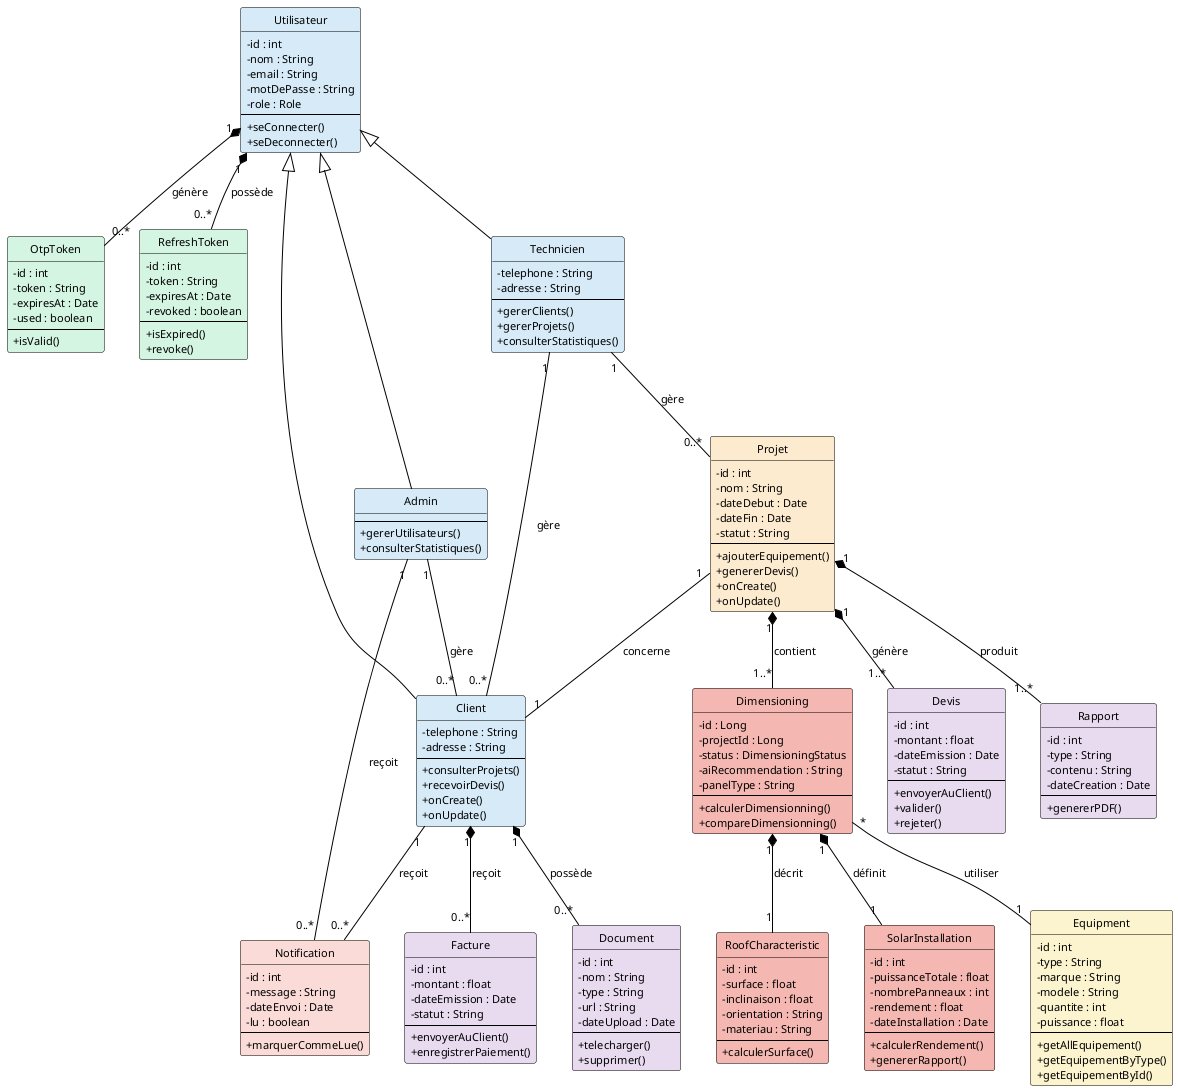
\includegraphics[width=0.92\textwidth]{diagramme-classe-globale.png}
  \caption{Diagramme de classes globale de SolarEase}
  \label{fig:class-diagram}
\end{figure}

\cleardoublepage


\chapterpage{3}{Sprints 1 et 2~: Fondation et Gestion Client/Projet}
% ============================================================
%  09-release1.tex
%  Chapitre 3 : Sprints 1 et 2 -- Fondation et Gestion Client/Projet
%  Contient : Sprint 1 (Identity) + Sprint 2 (Clients & Projets)
% ============================================================
\chapter{Sprints 1 et 2~: Fondation et Gestion Client/Projet}

% ══════════════════════════════════════════════════════════
\section{Sprint 1~: Service d'Identité et Authentification}
% ══════════════════════════════════════════════════════════

\subsection{Backlog du sprint}

{\small
\setlength{\LTleft}{0pt}
\setlength{\LTright}{0pt}
\begin{longtable}{|C{0.8cm}|L{4.2cm}|>{\raggedright\arraybackslash}p{\dimexpr\textwidth-0.8cm-4.2cm-1.5cm-8\tabcolsep-5\arrayrulewidth\relax}|C{1.5cm}|}
  \caption{Backlog Kanban -- Sprint 1 (Identity Service, Port 8081)}\label{tab:backlog-s1}\\
  \hline
  \rowcolor{figblue}
  \textcolor{white}{\textbf{ID}} &
  \textcolor{white}{\textbf{User Story}} &
  \textcolor{white}{\textbf{Tâches}} &
  \textcolor{white}{\textbf{Effort}} \\
  \hline
  \endfirsthead

  \hline
  \rowcolor{figblue}
  \textcolor{white}{\textbf{ID}} &
  \textcolor{white}{\textbf{User Story}} &
  \textcolor{white}{\textbf{Tâches}} &
  \textcolor{white}{\textbf{Effort}} \\
  \hline
  \endhead

  \hline
  \multicolumn{4}{r}{\small\textit{Suite page suivante}}\\
  \endfoot

  \hline
  \endlastfoot

  1 & En tant que client, je veux créer un compte avec
    vérification e-mail pour accéder à mon espace. &
  $\rightarrow$ Endpoint \texttt{POST /register} (username, email, password, firstName, lastName, phone)\newline
  $\rightarrow$ Hash BCrypt (force 10)\newline
  $\rightarrow$ Rôle automatiquement assigné à \texttt{CLIENT}\newline
  $\rightarrow$ Génération OTP 6 chiffres (TTL 10 min)\newline
  $\rightarrow$ Envoi OTP par e-mail (SMTP)\newline
  $\rightarrow$ Endpoints \texttt{POST /verify-otp} et \texttt{POST /resend-otp}\newline
  $\rightarrow$ Interface React (formulaire + page OTP)\newline
  $\rightarrow$ Tests unitaires et intégration & Élevé \\
  \hline
  2 & En tant qu'admin, je veux créer et gérer les comptes
    installateurs de l'entreprise. &
  $\rightarrow$ Endpoint \texttt{POST /api/auth/installers} (firstName, lastName, email, phone, password)\newline
  $\rightarrow$ Endpoints \texttt{GET}, \texttt{PUT}, \texttt{DELETE /api/auth/installers/\{uuid\}}\newline
  $\rightarrow$ Compte créé directement vérifié (\texttt{isEmailVerified=true})\newline
  $\rightarrow$ Interface admin de gestion des installateurs\newline
  $\rightarrow$ Vérification du rôle \texttt{ADMIN} obligatoire & Élevé \\
  \hline
  3 & En tant qu'utilisateur (client ou installateur), je veux me connecter
    et obtenir un token JWT pour accéder aux services. &
  $\rightarrow$ Endpoint \texttt{POST /login}\newline
  $\rightarrow$ Génération Access Token (HS256, 1h) avec claims \texttt{role}, \texttt{email}\newline
  $\rightarrow$ Génération Refresh Token (UUID, 7j)\newline
  $\rightarrow$ Endpoint \texttt{POST /refresh} (rotation)\newline
  $\rightarrow$ Réponse \texttt{AuthResponse} enrichie (tokens + \texttt{UserDto})\newline
  $\rightarrow$ Interface login React + redirection selon le rôle\newline
  $\rightarrow$ Tests avec Postman & Élevé \\
  \hline
  4 & En tant qu'utilisateur connecté, je veux consulter et
    modifier mon profil. &
  $\rightarrow$ Endpoints \texttt{GET /me} et \texttt{PUT /me}\newline
  $\rightarrow$ Endpoint dédié \texttt{PUT /me/password} (ancien + nouveau mot de passe)\newline
  $\rightarrow$ Interface profil React\newline
  $\rightarrow$ Tests fonctionnels & Moyen \\
  \hline
  5 & En tant que système, le Gateway doit valider les JWT
    et propager l'identité aux services. &
  $\rightarrow$ Filtre JWT dans Spring Cloud Gateway\newline
  $\rightarrow$ Propagation \texttt{X-User-Id}, \texttt{X-User-Role}, \texttt{X-User-Email}\newline
  $\rightarrow$ Liste de routes publiques exemptées (register, login, OTP, etc.)\newline
  $\rightarrow$ Rejet automatique des tokens expirés (HTTP 401)\newline
  $\rightarrow$ Tests de sécurité (token valide/invalide) & Élevé \\
  \hline
\end{longtable}
}

\subsection{Analyse du sprint 1}

Pour mieux comprendre ce premier sprint, nous allons présenter le diagramme
de cas d'utilisation du sprint~1, décrire les différents cas d'utilisation,
et détailler les fonctionnalités mentionnées dans ce sprint.

\subsubsection{Diagramme de cas d'utilisation global relatif au sprint 1}

Ce diagramme de cas d'utilisation illustre les différentes fonctionnalités
prises en charge lors du sprint~1, accessibles aux deux acteurs principaux~:
l'\textbf{Admin}, qui crée et gère les comptes installateurs en interne, et
le \textbf{Client}, qui s'auto-inscrit via le formulaire public et gère son
propre profil. Les installateurs ne s'inscrivent pas eux-mêmes~; leurs comptes
sont provisionnés par l'administrateur.

\begin{figure}[H]
  \centering
  \IfFileExists{101.png}{%
    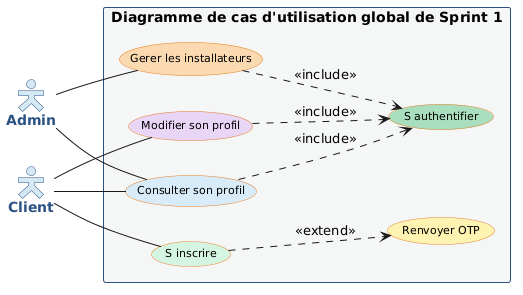
\includegraphics[width=0.88\textwidth]{101.png}%
  }{%
    \fbox{\parbox[c][8cm][c]{0.92\textwidth}{\centering Diagramme de cas d'utilisation global de Sprint 1}}%
  }
  \caption{Diagramme de cas d'utilisation global de Sprint~1}
  \label{fig:uc-s1}
\end{figure}

\subsubsection{Vue détaillée des cas d'utilisation développés durant le sprint 1}

Ensuite, nous présentons les diagrammes de cas d'utilisation détaillés
correspondant aux fonctionnalités principales. Ces diagrammes permettent
de mieux illustrer les interactions entre les acteurs et le système.

% ──────────────────────────────────────────────
\paragraph{Raffinement de cas d'utilisation «~Gérer les installateurs~»}

\begin{figure}[H]
  \centering
  \IfFileExists{102.png}{%
    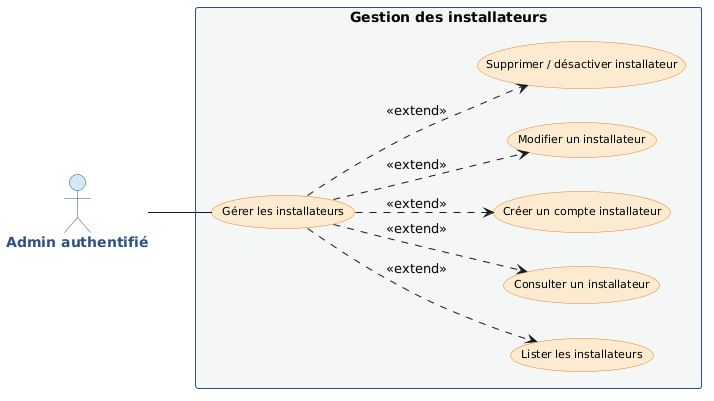
\includegraphics[width=0.85\textwidth]{102.png}%
  }{%
    \fbox{\parbox[c][6cm][c]{0.85\textwidth}{\centering Diagramme de cas d'utilisation -- Gérer les installateurs}}%
  }
  \caption{Diagramme de cas d'utilisation pour «~Gérer les installateurs~»}
  \label{fig:uc-installateurs}
\end{figure}

\subparagraph{Description textuelle du cas d'utilisation «~Créer un compte installateur~»}

\begin{table}[H]
  \caption{Description textuelle du cas d'utilisation «~Créer un compte installateur~»}
  \label{tab:cu-creer-installateur}
  \centering
  \begin{tabularx}{\textwidth}{|L{3.8cm}|X|}
    \hline
    \rowcolor{figblue!10}
    \textbf{Cas d'utilisation} & Créer un compte installateur. \\
    \hline
    \textbf{Acteur initiateur} & Administrateur \\
    \hline
    \textbf{But du cas} & Permettre à l'administrateur d'ajouter un nouveau compte installateur au système en saisissant les informations requises. \\
    \hline
    \textbf{Précondition} & L'administrateur doit être authentifié avec succès, l'e-mail de l'installateur n'existe pas dans la base. \\
    \hline
    \textbf{Description du scénario} &
    \textbf{Scénario principal :}\newline
    1. L'administrateur se connecte au système via l'interface d'authentification.\newline
    2. Il accède à la section «~Gestion des installateurs~».\newline
    3. Il clique sur le bouton «~Créer un compte installateur~».\newline
    4. Un formulaire d'ajout s'affiche.\newline
    5. L'administrateur saisit les informations nécessaires (prénom, nom, e-mail, téléphone, mot de passe).\newline
    6. Il valide le formulaire.\newline
    7. Le système hache le mot de passe (BCrypt, force~10) et enregistre le compte avec \texttt{isEmailVerified=true}, rôle \texttt{INSTALLER}.\newline
    8. Le système affiche un message de confirmation et met à jour la liste des installateurs.\\
    \hline
    \textbf{Scénarios alternatifs} &
    \textit{Scénario alternatif 1 -- Installateur déjà existant :}\newline
    \hspace*{6pt}7.1.~L'administrateur saisit un e-mail déjà enregistré.\newline
    \hspace*{6pt}7.2.~Le système affiche un message d'erreur~: «~Installateur déjà existant~».\newline[2pt]
    \textit{Scénario alternatif 2 -- Rôle insuffisant :}\newline
    \hspace*{6pt}1.1.~Un utilisateur non administrateur tente d'accéder à la route.\newline
    \hspace*{6pt}1.2.~Le Gateway renvoie HTTP~403 et refuse l'accès.\\
    \hline
  \end{tabularx}
\end{table}

\subparagraph{Description textuelle du cas d'utilisation «~Modifier un installateur~»}

\begin{table}[H]
  \caption{Description textuelle du cas d'utilisation «~Modifier un installateur~»}
  \label{tab:cu-modifier-installateur}
  \centering
  \begin{tabularx}{\textwidth}{|L{3.8cm}|X|}
    \hline
    \rowcolor{figblue!10}
    \textbf{Cas d'utilisation} & Modifier un installateur. \\
    \hline
    \textbf{Acteur initiateur} & Administrateur \\
    \hline
    \textbf{But du cas} & Permettre à l'administrateur de modifier les informations d'un compte installateur déjà existant (nom, prénom, téléphone, e-mail, statut actif). \\
    \hline
    \textbf{Précondition} & L'administrateur est authentifié et l'installateur ciblé existe dans la base. \\
    \hline
    \textbf{Description du scénario} &
    \textbf{Scénario principal :}\newline
    1. L'administrateur se connecte au système.\newline
    2. Il accède à la section «~Gestion des installateurs~».\newline
    3. Le système affiche la liste des installateurs.\newline
    4. L'administrateur sélectionne un installateur à modifier.\newline
    5. Il saisit les modifications souhaitées dans le formulaire prérempli.\newline
    6. Le système valide les nouvelles données.\newline
    7. Le système enregistre les modifications et affiche un message de confirmation.\newline
    8. La liste des installateurs est mise à jour.\\
    \hline
    \textbf{Scénarios alternatifs} &
    \textit{Scénario alternatif 1 -- Installateur introuvable :}\newline
    \hspace*{6pt}4.1.~L'identifiant ne correspond à aucun installateur.\newline
    \hspace*{6pt}4.2.~Le système renvoie HTTP~404 : «~Installateur introuvable~».\newline[2pt]
    \textit{Scénario alternatif 2 -- E-mail déjà utilisé :}\newline
    \hspace*{6pt}6.1.~Le nouvel e-mail est déjà attribué à un autre compte.\newline
    \hspace*{6pt}6.2.~Le système renvoie HTTP~409 et affiche un message d'erreur.\\
    \hline
  \end{tabularx}
\end{table}

\subparagraph{Description textuelle du cas d'utilisation «~Supprimer / désactiver un installateur~»}

\begin{table}[H]
  \caption{Description textuelle du cas d'utilisation «~Supprimer / désactiver un installateur~»}
  \label{tab:cu-supprimer-installateur}
  \centering
  \begin{tabularx}{\textwidth}{|L{3.8cm}|X|}
    \hline
    \rowcolor{figblue!10}
    \textbf{Cas d'utilisation} & Supprimer / désactiver un installateur. \\
    \hline
    \textbf{Acteur initiateur} & Administrateur \\
    \hline
    \textbf{But du cas} & Permettre à l'administrateur de retirer un installateur de la plateforme par une suppression logique (\texttt{isActive=false}), préservant ainsi l'historique des projets et clients associés. \\
    \hline
    \textbf{Précondition} & L'administrateur est authentifié et l'installateur ciblé existe. \\
    \hline
    \textbf{Description du scénario} &
    \textbf{Scénario principal :}\newline
    1. L'administrateur accède à la section «~Gestion des installateurs~».\newline
    2. Le système affiche la liste des installateurs.\newline
    3. L'administrateur sélectionne un installateur à désactiver.\newline
    4. Il clique sur le bouton «~Désactiver~».\newline
    5. Le système demande une confirmation.\newline
    6. L'administrateur confirme l'action.\newline
    7. Le système met à jour le statut (\texttt{isActive=false}) et révoque tous les Refresh Tokens de l'installateur.\newline
    8. Un message de confirmation s'affiche.\\
    \hline
    \textbf{Scénarios alternatifs} &
    \textit{Scénario alternatif 1 -- Annulation :}\newline
    \hspace*{6pt}5.1.~L'administrateur annule la confirmation.\newline
    \hspace*{6pt}5.2.~Aucune modification n'est appliquée.\newline[2pt]
    \textit{Scénario alternatif 2 -- Installateur avec projets actifs :}\newline
    \hspace*{6pt}6.1.~Le système alerte sur la présence de projets en cours.\newline
    \hspace*{6pt}6.2.~L'administrateur doit confirmer ou réaffecter les projets avant désactivation.\\
    \hline
  \end{tabularx}
\end{table}

\subparagraph{Description textuelle du cas d'utilisation «~Lister les installateurs~»}

\begin{table}[H]
  \caption{Description textuelle du cas d'utilisation «~Lister les installateurs~»}
  \label{tab:cu-lister-installateurs}
  \centering
  \begin{tabularx}{\textwidth}{|L{3.8cm}|X|}
    \hline
    \rowcolor{figblue!10}
    \textbf{Cas d'utilisation} & Lister les installateurs. \\
    \hline
    \textbf{Acteur initiateur} & Administrateur \\
    \hline
    \textbf{But du cas} & Permettre à l'administrateur de visualiser l'ensemble des comptes installateurs enregistrés, avec leurs informations principales (nom, e-mail, statut, date de création). \\
    \hline
    \textbf{Précondition} & L'administrateur doit être authentifié avec succès. \\
    \hline
    \textbf{Description du scénario} &
    \textbf{Scénario principal :}\newline
    1. L'administrateur se connecte au système.\newline
    2. Il accède à la section «~Gestion des installateurs~».\newline
    3. Le système envoie une requête \texttt{GET /api/auth/installers}.\newline
    4. Le système récupère tous les utilisateurs de rôle \texttt{INSTALLER}.\newline
    5. La liste est affichée sous forme de tableau paginé avec filtres (statut, recherche par nom).\newline
    6. L'administrateur peut trier, filtrer ou cliquer sur un installateur pour le consulter.\\
    \hline
    \textbf{Scénarios alternatifs} &
    \textit{Scénario alternatif 1 -- Aucun installateur :}\newline
    \hspace*{6pt}5.1.~La base ne contient aucun installateur.\newline
    \hspace*{6pt}5.2.~Le système affiche : «~Aucun installateur enregistré~».\newline[2pt]
    \textit{Scénario alternatif 2 -- Erreur serveur :}\newline
    \hspace*{6pt}3.1.~Le service d'identité est indisponible.\newline
    \hspace*{6pt}3.2.~Le système affiche un message d'erreur et propose de réessayer.\\
    \hline
  \end{tabularx}
\end{table}

% ──────────────────────────────────────────────
\paragraph{Raffinement de cas d'utilisation «~S'inscrire~»}

\begin{figure}[H]
  \centering
  \IfFileExists{103.png}{%
    \includegraphics[width=0.85\textwidth]{103.png}%
  }{%
    \fbox{\parbox[c][6cm][c]{0.85\textwidth}{\centering Diagramme de cas d'utilisation -- S'inscrire}}%
  }
  \caption{Diagramme de cas d'utilisation pour «~S'inscrire~»}
  \label{fig:uc-sinscrire}
\end{figure}

\subparagraph{Description textuelle du cas d'utilisation «~S'inscrire~»}

\begin{table}[H]
  \caption{Description textuelle du cas d'utilisation «~S'inscrire~»}
  \label{tab:cu-sinscrire}
  \centering
  \begin{tabularx}{\textwidth}{|L{3.8cm}|X|}
    \hline
    \rowcolor{figblue!10}
    \textbf{Cas d'utilisation} & S'inscrire sur la plateforme SolarEase. \\
    \hline
    \textbf{Acteur initiateur} & Visiteur (futur client) \\
    \hline
    \textbf{But du cas} & Permettre à un visiteur de créer un compte client en vérifiant son adresse e-mail par un code OTP, afin d'accéder à son espace personnel. \\
    \hline
    \textbf{Précondition} & L'adresse e-mail n'existe pas déjà dans la base. \\
    \hline
    \textbf{Description du scénario} &
    \textbf{Scénario principal :}\newline
    1. Le visiteur accède au formulaire d'inscription public.\newline
    2. Il saisit ses informations (nom, prénom, e-mail, téléphone, mot de passe).\newline
    3. Le système valide les champs et hache le mot de passe (BCrypt, force~10).\newline
    4. Le compte est créé avec \texttt{isEmailVerified=false} et rôle \texttt{CLIENT}.\newline
    5. Le système génère un code OTP à 6~chiffres (TTL 10~min) et l'envoie par e-mail.\newline
    6. Le visiteur est redirigé vers la page de vérification OTP.\newline
    7. Il saisit le code reçu.\newline
    8. Le système valide l'OTP et active le compte (\texttt{isEmailVerified=true}).\newline
    9. Le visiteur peut alors se connecter.\\
    \hline
    \textbf{Scénarios alternatifs} &
    \textit{Scénario alternatif 1 -- E-mail déjà utilisé :}\newline
    \hspace*{6pt}3.1.~Le système détecte un e-mail existant et renvoie HTTP~409.\newline[2pt]
    \textit{Scénario alternatif 2 -- OTP expiré :}\newline
    \hspace*{6pt}7.1.~Le code saisi est expiré ($>$10~min).\newline
    \hspace*{6pt}7.2.~Le système propose le renvoi d'un nouveau code (\texttt{POST /resend-otp}).\\
    \hline
  \end{tabularx}
\end{table}

\subparagraph{Description textuelle du cas d'utilisation «~Vérifier le code OTP~»}

\begin{table}[H]
  \caption{Description textuelle du cas d'utilisation «~Vérifier le code OTP~»}
  \label{tab:cu-verifier-otp}
  \centering
  \begin{tabularx}{\textwidth}{|L{3.8cm}|X|}
    \hline
    \rowcolor{figblue!10}
    \textbf{Cas d'utilisation} & Vérifier le code OTP. \\
    \hline
    \textbf{Acteur initiateur} & Visiteur inscrit (compte non encore activé) \\
    \hline
    \textbf{But du cas} & Permettre au visiteur d'activer son compte en confirmant la réception du code OTP envoyé à son adresse e-mail. \\
    \hline
    \textbf{Précondition} & Le compte existe avec \texttt{isEmailVerified=false} et un OTP valide est présent en base (non utilisé et non expiré). \\
    \hline
    \textbf{Description du scénario} &
    \textbf{Scénario principal :}\newline
    1. Le visiteur est redirigé sur la page de vérification.\newline
    2. Il consulte sa boîte e-mail et récupère le code à 6~chiffres.\newline
    3. Il saisit le code dans le formulaire.\newline
    4. Le système recherche l'OTP en base (par e-mail + code).\newline
    5. Vérification : token non utilisé et non expiré ($<$10~min).\newline
    6. Le système marque l'OTP comme utilisé (\texttt{used=true}).\newline
    7. Le compte est activé (\texttt{isEmailVerified=true}).\newline
    8. Un message de confirmation est affiché et l'utilisateur est redirigé vers la page de connexion.\\
    \hline
    \textbf{Scénarios alternatifs} &
    \textit{Scénario alternatif 1 -- Code incorrect :}\newline
    \hspace*{6pt}4.1.~Aucun OTP ne correspond au code saisi.\newline
    \hspace*{6pt}4.2.~Le système renvoie HTTP~400 : «~Code OTP incorrect~».\newline[2pt]
    \textit{Scénario alternatif 2 -- OTP expiré :}\newline
    \hspace*{6pt}5.1.~L'OTP est en base mais expiré.\newline
    \hspace*{6pt}5.2.~Le système propose de demander un nouveau code.\newline[2pt]
    \textit{Scénario alternatif 3 -- OTP déjà utilisé :}\newline
    \hspace*{6pt}5.3.~Le champ \texttt{used} est déjà à \texttt{true}.\newline
    \hspace*{6pt}5.4.~Le système rejette la requête.\\
    \hline
  \end{tabularx}
\end{table}

\subparagraph{Description textuelle du cas d'utilisation «~Renvoyer un OTP~»}

\begin{table}[H]
  \caption{Description textuelle du cas d'utilisation «~Renvoyer un OTP~»}
  \label{tab:cu-renvoyer-otp}
  \centering
  \begin{tabularx}{\textwidth}{|L{3.8cm}|X|}
    \hline
    \rowcolor{figblue!10}
    \textbf{Cas d'utilisation} & Renvoyer un code OTP. \\
    \hline
    \textbf{Acteur initiateur} & Visiteur inscrit (compte non activé) \\
    \hline
    \textbf{But du cas} & Permettre au visiteur de demander un nouveau code OTP s'il n'a pas reçu le précédent ou si celui-ci a expiré. \\
    \hline
    \textbf{Précondition} & Le compte existe avec \texttt{isEmailVerified=false}. \\
    \hline
    \textbf{Description du scénario} &
    \textbf{Scénario principal :}\newline
    1. Le visiteur clique sur le lien «~Renvoyer le code~» dans la page de vérification.\newline
    2. Le système vérifie le délai anti-flood (1 demande / 60~secondes).\newline
    3. L'ancien OTP est invalidé (\texttt{used=true}).\newline
    4. Le système génère un nouveau code à 6~chiffres avec un nouveau TTL de 10~minutes.\newline
    5. Le code est enregistré en base et envoyé par e-mail.\newline
    6. Un message de confirmation s'affiche : «~Code renvoyé~».\\
    \hline
    \textbf{Scénarios alternatifs} &
    \textit{Scénario alternatif 1 -- Anti-flood actif :}\newline
    \hspace*{6pt}2.1.~Une demande a déjà été faite il y a moins de 60~secondes.\newline
    \hspace*{6pt}2.2.~Le système renvoie HTTP~429 : «~Veuillez patienter avant de redemander un code~».\newline[2pt]
    \textit{Scénario alternatif 2 -- Compte déjà activé :}\newline
    \hspace*{6pt}1.1.~Le compte est déjà vérifié.\newline
    \hspace*{6pt}1.2.~Le système redirige vers la page de connexion.\\
    \hline
  \end{tabularx}
\end{table}

% ──────────────────────────────────────────────
\paragraph{Raffinement de cas d'utilisation «~Modifier son profil~»}

\begin{figure}[H]
  \centering
  \IfFileExists{104.png}{%
    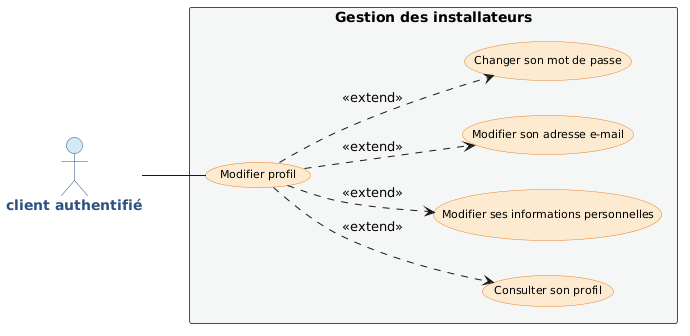
\includegraphics[width=0.85\textwidth]{104.png}%
  }{%
    \fbox{\parbox[c][6cm][c]{0.85\textwidth}{\centering Diagramme de cas d'utilisation -- Modifier son profil}}%
  }
  \caption{Diagramme de cas d'utilisation pour «~Modifier son profil~»}
  \label{fig:uc-profil}
\end{figure}

\subparagraph{Description textuelle du cas d'utilisation «~Changer son mot de passe~»}

\begin{table}[H]
  \caption{Description textuelle du cas d'utilisation «~Changer son mot de passe~»}
  \label{tab:cu-changer-mdp}
  \centering
  \begin{tabularx}{\textwidth}{|L{3.8cm}|X|}
    \hline
    \rowcolor{figblue!10}
    \textbf{Cas d'utilisation} & Changer son mot de passe. \\
    \hline
    \textbf{Acteur initiateur} & Client (ou tout utilisateur authentifié) \\
    \hline
    \textbf{But du cas} & Permettre à un utilisateur authentifié de modifier son mot de passe afin de renforcer la sécurité de son compte. \\
    \hline
    \textbf{Précondition} & L'utilisateur est authentifié et connaît son ancien mot de passe. \\
    \hline
    \textbf{Description du scénario} &
    \textbf{Scénario principal :}\newline
    1. L'utilisateur s'authentifie dans le système.\newline
    2. Il accède à la section «~Mon profil~».\newline
    3. Il clique sur «~Changer mot de passe~».\newline
    4. Il saisit son ancien mot de passe puis le nouveau (deux fois).\newline
    5. Le système vérifie l'ancien mot de passe (comparaison BCrypt).\newline
    6. Le système valide la force du nouveau mot de passe ($\geq$~8 caractères).\newline
    7. Le nouveau mot de passe est haché et enregistré.\newline
    8. Tous les Refresh Tokens existants sont révoqués.\newline
    9. Le système envoie une notification e-mail d'alerte sécurité.\newline
    10. Un message de confirmation s'affiche.\\
    \hline
    \textbf{Scénarios alternatifs} &
    \textit{Scénario alternatif 1 -- Ancien mot de passe incorrect :}\newline
    \hspace*{6pt}5.1.~Le système renvoie HTTP~401.\newline
    \hspace*{6pt}5.2.~Le formulaire affiche~: «~Ancien mot de passe incorrect~».\newline[2pt]
    \textit{Scénario alternatif 2 -- Nouveau mot de passe trop faible :}\newline
    \hspace*{6pt}6.1.~Le système renvoie une erreur de validation.\newline
    \hspace*{6pt}6.2.~Le formulaire indique les exigences (longueur, complexité).\\
    \hline
  \end{tabularx}
\end{table}

\subparagraph{Description textuelle du cas d'utilisation «~Modifier son adresse e-mail~»}

\begin{table}[H]
  \caption{Description textuelle du cas d'utilisation «~Modifier son adresse e-mail~»}
  \label{tab:cu-modifier-email}
  \centering
  \begin{tabularx}{\textwidth}{|L{3.8cm}|X|}
    \hline
    \rowcolor{figblue!10}
    \textbf{Cas d'utilisation} & Modifier son adresse e-mail. \\
    \hline
    \textbf{Acteur initiateur} & Utilisateur authentifié (Client, Installateur ou Admin) \\
    \hline
    \textbf{But du cas} & Permettre à l'utilisateur de changer l'adresse e-mail associée à son compte avec re-vérification obligatoire par OTP. \\
    \hline
    \textbf{Précondition} & L'utilisateur est authentifié et la nouvelle adresse n'est pas déjà utilisée par un autre compte. \\
    \hline
    \textbf{Description du scénario} &
    \textbf{Scénario principal :}\newline
    1. L'utilisateur accède à la section «~Mon profil~».\newline
    2. Il clique sur «~Modifier mon e-mail~».\newline
    3. Il saisit la nouvelle adresse e-mail.\newline
    4. Le système valide le format et l'unicité de l'adresse.\newline
    5. Le système génère un OTP de confirmation et l'envoie à la nouvelle adresse.\newline
    6. L'utilisateur récupère le code et le saisit.\newline
    7. Le système valide l'OTP et applique la nouvelle adresse (\texttt{user.email = nouveau}).\newline
    8. Tous les Refresh Tokens existants sont révoqués.\newline
    9. Un message de confirmation est affiché.\\
    \hline
    \textbf{Scénarios alternatifs} &
    \textit{Scénario alternatif 1 -- E-mail déjà utilisé :}\newline
    \hspace*{6pt}4.1.~La nouvelle adresse appartient à un autre compte.\newline
    \hspace*{6pt}4.2.~Le système renvoie HTTP~409 : «~Cette adresse e-mail est déjà utilisée~».\newline[2pt]
    \textit{Scénario alternatif 2 -- OTP non saisi à temps :}\newline
    \hspace*{6pt}6.1.~L'utilisateur n'a pas validé l'OTP dans les 10~minutes.\newline
    \hspace*{6pt}6.2.~La nouvelle adresse n'est pas appliquée, l'ancienne reste active.\\
    \hline
  \end{tabularx}
\end{table}

\subparagraph{Description textuelle du cas d'utilisation «~Modifier ses informations personnelles~»}

\begin{table}[H]
  \caption{Description textuelle du cas d'utilisation «~Modifier ses informations personnelles~»}
  \label{tab:cu-modifier-infos}
  \centering
  \begin{tabularx}{\textwidth}{|L{3.8cm}|X|}
    \hline
    \rowcolor{figblue!10}
    \textbf{Cas d'utilisation} & Modifier ses informations personnelles. \\
    \hline
    \textbf{Acteur initiateur} & Utilisateur authentifié \\
    \hline
    \textbf{But du cas} & Permettre à l'utilisateur de mettre à jour ses informations personnelles (prénom, nom, téléphone, adresse postale) sans validation supplémentaire par OTP. \\
    \hline
    \textbf{Précondition} & L'utilisateur est authentifié avec succès. \\
    \hline
    \textbf{Description du scénario} &
    \textbf{Scénario principal :}\newline
    1. L'utilisateur accède à la section «~Mon profil~».\newline
    2. Le système affiche le formulaire prérempli avec ses informations actuelles.\newline
    3. L'utilisateur modifie les champs souhaités (prénom, nom, téléphone, adresse).\newline
    4. Il valide le formulaire.\newline
    5. Le système valide les données (Jakarta Validation).\newline
    6. Les nouvelles informations sont enregistrées en base.\newline
    7. Un message de confirmation est affiché.\\
    \hline
    \textbf{Scénarios alternatifs} &
    \textit{Scénario alternatif 1 -- Données invalides :}\newline
    \hspace*{6pt}5.1.~Le numéro de téléphone est mal formé ou un champ obligatoire est vide.\newline
    \hspace*{6pt}5.2.~Le système renvoie HTTP~400 avec le détail des erreurs.\newline
    \hspace*{6pt}5.3.~L'utilisateur corrige et revient à l'étape~4.\\
    \hline
  \end{tabularx}
\end{table}

\subparagraph{Description textuelle du cas d'utilisation «~Consulter son profil~»}

\begin{table}[H]
  \caption{Description textuelle du cas d'utilisation «~Consulter son profil~»}
  \label{tab:cu-consulter-profil}
  \centering
  \begin{tabularx}{\textwidth}{|L{3.8cm}|X|}
    \hline
    \rowcolor{figblue!10}
    \textbf{Cas d'utilisation} & Consulter son profil. \\
    \hline
    \textbf{Acteur initiateur} & Utilisateur authentifié \\
    \hline
    \textbf{But du cas} & Permettre à l'utilisateur de visualiser l'ensemble des informations de son compte (sans exposer les données sensibles). \\
    \hline
    \textbf{Précondition} & L'utilisateur est authentifié avec un JWT valide. \\
    \hline
    \textbf{Description du scénario} &
    \textbf{Scénario principal :}\newline
    1. L'utilisateur accède à la section «~Mon profil~».\newline
    2. Le frontend envoie une requête \texttt{GET /api/auth/me}.\newline
    3. Le Gateway valide le JWT et propage l'identifiant.\newline
    4. Le système récupère l'utilisateur en base.\newline
    5. Le système retourne un \texttt{UserDto} (id, e-mail, prénom, nom, téléphone, rôle, date de création).\newline
    6. Le frontend affiche les informations dans la page «~Mon profil~».\\
    \hline
    \textbf{Scénarios alternatifs} &
    \textit{Scénario alternatif 1 -- Session expirée :}\newline
    \hspace*{6pt}3.1.~Le JWT est expiré ou invalide.\newline
    \hspace*{6pt}3.2.~Le Gateway renvoie HTTP~401.\newline
    \hspace*{6pt}3.3.~Le frontend tente un \texttt{refresh} automatique, sinon redirige vers la page de connexion.\\
    \hline
  \end{tabularx}
\end{table}

\subsection{Conception du sprint 1}

L'analyse conceptuelle de ce premier sprint comprendra la description des
diagrammes de séquence liés aux fonctionnalités majeures du sprint~1. Elle
se conclura par l'élaboration du diagramme de classes, synthétisant
l'ensemble des éléments étudiés.

\subsubsection{Diagrammes de séquence}

Dans cette phase, nous présentons les diagrammes de séquence correspondant
aux principales fonctionnalités développées lors du sprint~1. Ces diagrammes
illustrent les interactions entre les différents composants du système pour
chaque fonctionnalité ciblée.

% ──────────────────────────────────────────────
\paragraph{Diagramme de séquence «~S'authentifier~»}

La figure ci-après présente le scénario de connexion d'un utilisateur
(Admin, Installateur ou Client) avec génération d'un JWT par le service
d'identité.

\begin{figure}[H]
  \centering
  \IfFileExists{seq-sauthentifier.png}{%
    \includegraphics[width=0.95\textwidth,height=0.55\textheight,keepaspectratio]{seq-sauthentifier.png}%
  }{%
    \fbox{\parbox[c][7cm][c]{0.92\textwidth}{\centering Diagramme de séquence «~S'authentifier~»}}%
  }
  \caption{Diagramme de séquence «~S'authentifier~»}
  \label{fig:seq-sauthentifier}
\end{figure}

% ──────────────────────────────────────────────
\paragraph{Diagramme de séquence «~Créer un compte installateur~»}

La figure ci-après présente le cas d'utilisation de la création d'un
compte installateur par l'administrateur.

\begin{figure}[H]
  \centering
  \IfFileExists{seq-creer-installateur.png}{%
    \includegraphics[width=0.95\textwidth,height=0.55\textheight,keepaspectratio]{seq-creer-installateur.png}%
  }{%
    \fbox{\parbox[c][7cm][c]{0.92\textwidth}{\centering Diagramme de séquence «~Créer un compte installateur~»}}%
  }
  \caption{Diagramme de séquence «~Créer un compte installateur~»}
  \label{fig:seq-creer-installateur}
\end{figure}

% ──────────────────────────────────────────────
\paragraph{Diagramme de séquence «~S'inscrire~»}

La figure ci-après présente le cas d'utilisation de l'inscription d'un
client avec génération et vérification du code OTP.

\begin{figure}[H]
  \centering
  \IfFileExists{seq-sinscrire.png}{%
    \includegraphics[width=0.95\textwidth,height=0.7\textheight,keepaspectratio]{seq-sinscrire.png}%
  }{%
    \fbox{\parbox[c][8cm][c]{0.92\textwidth}{\centering Diagramme de séquence «~S'inscrire~»}}%
  }
  \caption{Diagramme de séquence «~S'inscrire~»}
  \label{fig:seq-sinscrire}
\end{figure}

% ──────────────────────────────────────────────
\paragraph{Diagramme de séquence «~Changer son mot de passe~»}

La figure ci-après présente le cas d'utilisation de la modification du
mot de passe par un utilisateur authentifié.

\begin{figure}[H]
  \centering
  \IfFileExists{seq-changer-mdp.png}{%
    \includegraphics[width=0.95\textwidth,height=0.6\textheight,keepaspectratio]{seq-changer-mdp.png}%
  }{%
    \fbox{\parbox[c][7cm][c]{0.92\textwidth}{\centering Diagramme de séquence «~Changer son mot de passe~»}}%
  }
  \caption{Diagramme de séquence «~Changer son mot de passe~»}
  \label{fig:seq-changer-mdp}
\end{figure}

\subsubsection{Diagramme de classes du sprint 1}

Ce diagramme de classes global illustre l'architecture du projet, avec les
classes liées au sprint~1.

Il permet d'identifier clairement les entités utilisées lors de ce premier
sprint.

\begin{figure}[H]
  \centering
  \includegraphics[width=0.85\textwidth]{class-sprint1.png}
  \caption{Diagramme de classes global du sprint~1}
  \label{fig:class-s1}
\end{figure}

\subsection{Réalisation du sprint 1}

Cette section présente les interfaces développées et les résultats de validation
du sprint~1.

\begin{lstlisting}[caption={JwtTokenProvider.java --- Génération du token d'accès},
                   label=lst:jwt, language=Java]
@Component
public class JwtTokenProvider {

    public String generateAccessToken(User user) {
        Date now    = new Date();
        Date expiry = new Date(now.getTime() + accessTokenExpMs);
        return Jwts.builder()
            .subject(user.getUuid().toString())
            .claim("role",  user.getRole().name())
            .claim("email", user.getEmail())
            .issuedAt(now).expiration(expiry)
            .signWith(getSigningKey(), Jwts.SIG.HS256)
            .compact();
    }

    public boolean validateToken(String token) {
        try {
            Jwts.parser().verifyWith(getSigningKey())
                .build().parseSignedClaims(token);
            return true;
        } catch (JwtException e) { return false; }
    }
}
\end{lstlisting}

\begin{table}[H]
  \caption{Résultats des tests fonctionnels -- Sprint 1}
  \label{tab:tests-s1}
  \centering\small
  \begin{tabularx}{\textwidth}{|C{1.2cm}|L{3.5cm}|X|C{1.4cm}|}
    \hline
    \rowcolor{figblue!20}
    \textbf{ID} & \textbf{Cas de test} & \textbf{Résultat attendu} & \textbf{Statut} \\
    \hline
    T-01 & Inscription client valide & HTTP 201 + OTP envoyé (rôle CLIENT) & \ok~OK \\
    \hline
    T-02 & Email déjà existant & HTTP 409 Conflict & \ok~OK \\
    \hline
    T-03 & OTP correct $<$10 min & Compte activé + tokens & \ok~OK \\
    \hline
    T-04 & OTP expiré & HTTP 400 "OTP expiré" & \ok~OK \\
    \hline
    T-05 & Connexion valide & Access + Refresh tokens & \ok~OK \\
    \hline
    T-06 & Mot de passe faux & HTTP 401 générique & \ok~OK \\
    \hline
    T-07 & Admin crée installateur & HTTP 201, compte vérifié INSTALLER & \ok~OK \\
    \hline
    T-08 & Création installateur sans rôle ADMIN & HTTP 403 Forbidden & \ok~OK \\
    \hline
    T-09 & JWT valide au Gateway & Propagation X-User-Id & \ok~OK \\
    \hline
    T-10 & JWT expiré au Gateway & HTTP 401 & \ok~OK \\
    \hline
  \end{tabularx}
\end{table}

\begin{figure}[H]
  \centering
  \IfFileExists{images/login.png}{%
    \includegraphics[width=0.85\textwidth]{images/login.png}%
  }{%
    \fbox{\parbox{0.85\textwidth}{
      \centering\vspace{0.5cm}
      \textit{Interface de connexion -- SolarEase}\\[4pt]
      \small Remplacer par : \texttt{\textbackslash includegraphics[width=0.85\textbackslash textwidth]\{images/login.png\}}\\[4pt]
      Formulaire email + mot de passe, logo SolarEase, lien inscription
      \vspace{0.5cm}
    }}%
  }
  \caption{Interface d'authentification -- SolarEase}
  \label{fig:ui-login}
\end{figure}

\begin{figure}[H]
  \centering
  \fbox{\parbox{0.85\textwidth}{
    \centering\vspace{0.5cm}
    \textit{Page de vérification OTP}\\[4pt]
    \small Remplacer par : \texttt{\textbackslash includegraphics[width=0.85\textbackslash textwidth]\{images/otp-verify.png\}}\\[4pt]
    6 champs de saisie, compte à rebours 10 min, bouton renvoi
    \vspace{0.5cm}
  }}
  \caption{Interface de vérification OTP -- Sprint 1}
  \label{fig:ui-otp}
\end{figure}

% ══════════════════════════════════════════════════════════
\section{Sprint 2~: Gestion des Clients et des Projets}
% ══════════════════════════════════════════════════════════

\subsection{Backlog du sprint}

\begin{table}[H]
  \caption{Backlog Kanban -- Sprint 2 (Project Service, Port 8082)}
  \label{tab:backlog-s2}
  \centering\small
  \begin{tabularx}{\textwidth}{|C{0.8cm}|L{4.2cm}|X|C{1.5cm}|}
    \hline
    \rowcolor{figblue}
    \textcolor{white}{\textbf{ID}} &
    \textcolor{white}{\textbf{User Story}} &
    \textcolor{white}{\textbf{Tâches}} &
    \textcolor{white}{\textbf{Effort}} \\
    \hline
    1 & En tant qu'admin, je veux gérer l'ensemble des clients
        de l'entreprise (ajouter, modifier, supprimer, consulter, chercher). &
    $\rightarrow$ Endpoints CRUD \texttt{/api/clients} (rôle \texttt{ADMIN})\newline
    $\rightarrow$ Vue globale~: l'admin liste tous les clients\newline
    $\rightarrow$ Pagination et recherche par nom/email\newline
    $\rightarrow$ Fiche détaillée client + projets liés\newline
    $\rightarrow$ Interfaces React (liste, formulaire, détail)\newline
    $\rightarrow$ Tests avec Postman puis intégration & Élevé \\
    \hline
    2 & En tant qu'admin, je veux créer les projets solaires
        et les affecter aux installateurs de l'entreprise. &
    $\rightarrow$ Endpoint dédié \texttt{POST /api/projects/admin/assign} (ADMIN uniquement)\newline
    $\rightarrow$ Liaison projet-client via \texttt{clientId} et projet-installateur via \texttt{installerId}\newline
    $\rightarrow$ Métadonnées d'affectation~: \texttt{assignedByAdminId}, \texttt{assignedByAdminEmail}\newline
    $\rightarrow$ Endpoints CRUD complémentaires \texttt{/api/projects}\newline
    $\rightarrow$ Gestion des 6 transitions de statut\newline
    $\rightarrow$ Interface admin~: formulaire création + sélection d'installateur\newline
    $\rightarrow$ Tests fonctionnels & Élevé \\
    \hline
    3 & En tant qu'admin, je veux visualiser un tableau
        de bord global avec les KPI de l'ensemble de l'entreprise. &
    $\rightarrow$ Endpoint \texttt{GET /api/projects/dashboard/stats} (vue globale pour ADMIN)\newline
    $\rightarrow$ Endpoint \texttt{GET /api/clients/stats}\newline
    $\rightarrow$ Requêtes JPQL agrégées (comptages globaux)\newline
    $\rightarrow$ Cartes KPI~: total clients, projets créés, en cours, terminés, annulés\newline
    $\rightarrow$ Interface dashboard admin avec filtres\newline
    $\rightarrow$ Tests & Moyen \\
    \hline
  \end{tabularx}
\end{table}

\subsection{Analyse du sprint 2}

Pour mieux comprendre ce deuxième sprint, nous allons présenter le diagramme
de cas d'utilisation du sprint~2, décrire les différents cas d'utilisation,
et détailler les fonctionnalités mentionnées dans ce sprint.

\subsubsection{Diagramme de cas d'utilisation global relatif au sprint 2}

Ce diagramme de cas d'utilisation illustre les différentes fonctionnalités
prises en charge lors du sprint~2, accessibles à deux acteurs~: l'\textbf{Admin},
qui gère l'intégralité du portefeuille clients et l'ensemble des projets de
l'entreprise (création, affectation, suivi, tableau de bord), et
l'\textbf{Installateur}, qui consulte ses projets affectés et fait évoluer
leur statut. Les clients ne sont pas représentés ici car leur interaction
sur les projets est traitée au sprint~5.

\begin{figure}[H]
  \centering
  \IfFileExists{uc-s2-global.png}{%
    \includegraphics[width=0.88\textwidth]{uc-s2-global.png}%
  }{%
    \fbox{\parbox[c][8cm][c]{0.92\textwidth}{\centering Diagramme de cas d'utilisation global de Sprint 2}}%
  }
  \caption{Diagramme de cas d'utilisation global de Sprint~2}
  \label{fig:uc-s2}
\end{figure}

\subsubsection{Vue détaillée des cas d'utilisation développés durant le sprint 2}

Ensuite, nous présentons les diagrammes de cas d'utilisation détaillés
correspondant aux fonctionnalités principales. Ces diagrammes permettent
de mieux illustrer les interactions entre les acteurs et le système.

% ──────────────────────────────────────────────
\paragraph{Raffinement de cas d'utilisation «~Gérer les clients~»}

\begin{figure}[H]
  \centering
  \IfFileExists{uc-admin-clients.png}{%
    \includegraphics[width=0.85\textwidth]{uc-admin-clients.png}%
  }{%
    \fbox{\parbox[c][6cm][c]{0.85\textwidth}{\centering Diagramme de cas d'utilisation -- Gérer les clients}}%
  }
  \caption{Diagramme de cas d'utilisation pour «~Gérer les clients~»}
  \label{fig:uc-clients}
\end{figure}

\subparagraph{Description textuelle du cas d'utilisation «~Créer une fiche client~»}

\begin{table}[H]
  \caption{Description textuelle du cas d'utilisation «~Créer une fiche client~»}
  \label{tab:cu-creer-client}
  \centering
  \begin{tabularx}{\textwidth}{|L{3.8cm}|X|}
    \hline
    \rowcolor{figblue!10}
    \textbf{Cas d'utilisation} & Créer une fiche client. \\
    \hline
    \textbf{Acteur initiateur} & Administrateur \\
    \hline
    \textbf{But du cas} & Permettre à l'administrateur d'ajouter une nouvelle fiche client au portefeuille de l'entreprise en saisissant les informations de contact requises. \\
    \hline
    \textbf{Précondition} & L'administrateur est authentifié avec un JWT valide portant le rôle \texttt{ADMIN} et l'e-mail du client n'existe pas déjà dans la base. \\
    \hline
    \textbf{Description du scénario} &
    \textbf{Scénario principal :}\newline
    1. L'administrateur accède à la section «~Gestion des clients~».\newline
    2. Il clique sur le bouton «~Nouveau client~».\newline
    3. Un formulaire d'ajout s'affiche.\newline
    4. Il saisit les informations (prénom, nom, e-mail, téléphone, adresse).\newline
    5. Le frontend valide les champs (schéma Zod).\newline
    6. Le système vérifie l'unicité de l'e-mail et persiste la fiche.\newline
    7. La fiche est enregistrée dans la table \texttt{items\_client}.\newline
    8. Un message de confirmation s'affiche et la liste est rafraîchie automatiquement.\\
    \hline
    \textbf{Scénarios alternatifs} &
    \textit{Scénario alternatif 1 -- E-mail déjà utilisé :}\newline
    \hspace*{6pt}6.1.~Le système détecte un e-mail existant.\newline
    \hspace*{6pt}6.2.~Le système renvoie HTTP~409 : «~E-mail déjà utilisé~».\newline[2pt]
    \textit{Scénario alternatif 2 -- Champ obligatoire manquant :}\newline
    \hspace*{6pt}5.1.~Le système renvoie HTTP~400 avec le détail des erreurs.\newline
    \hspace*{6pt}5.2.~L'utilisateur corrige les champs et revient à l'étape~4.\\
    \hline
  \end{tabularx}
\end{table}

\subparagraph{Description textuelle du cas d'utilisation «~Lister les clients~»}

\begin{table}[H]
  \caption{Description textuelle du cas d'utilisation «~Lister les clients~»}
  \label{tab:cu-lister-clients}
  \centering
  \begin{tabularx}{\textwidth}{|L{3.8cm}|X|}
    \hline
    \rowcolor{figblue!10}
    \textbf{Cas d'utilisation} & Lister les clients. \\
    \hline
    \textbf{Acteur initiateur} & Administrateur \\
    \hline
    \textbf{But du cas} & Permettre à l'administrateur de visualiser l'ensemble des fiches clients enregistrées dans le portefeuille, avec leurs informations principales. \\
    \hline
    \textbf{Précondition} & L'administrateur est authentifié avec succès. \\
    \hline
    \textbf{Description du scénario} &
    \textbf{Scénario principal :}\newline
    1. L'administrateur accède à la section «~Gestion des clients~».\newline
    2. Le frontend envoie une requête \texttt{GET /api/clients}.\newline
    3. Le système récupère tous les enregistrements de la table \texttt{items\_client}.\newline
    4. La liste est affichée sous forme de tableau paginé avec filtres (recherche par nom, e-mail, ville).\newline
    5. L'administrateur peut trier, filtrer ou cliquer sur un client pour le consulter.\\
    \hline
    \textbf{Scénarios alternatifs} &
    \textit{Scénario alternatif 1 -- Aucun client :}\newline
    \hspace*{6pt}3.1.~La base ne contient aucune fiche.\newline
    \hspace*{6pt}3.2.~Le système affiche : «~Aucun client enregistré~».\newline[2pt]
    \textit{Scénario alternatif 2 -- Erreur serveur :}\newline
    \hspace*{6pt}2.1.~Le service projet est indisponible.\newline
    \hspace*{6pt}2.2.~Le système affiche un message d'erreur et propose de réessayer.\\
    \hline
  \end{tabularx}
\end{table}

\subparagraph{Description textuelle du cas d'utilisation «~Consulter une fiche client~»}

\begin{table}[H]
  \caption{Description textuelle du cas d'utilisation «~Consulter une fiche client~»}
  \label{tab:cu-consulter-client}
  \centering
  \begin{tabularx}{\textwidth}{|L{3.8cm}|X|}
    \hline
    \rowcolor{figblue!10}
    \textbf{Cas d'utilisation} & Consulter une fiche client. \\
    \hline
    \textbf{Acteur initiateur} & Administrateur \\
    \hline
    \textbf{But du cas} & Permettre à l'administrateur de visualiser le détail d'une fiche client, y compris les projets associés. \\
    \hline
    \textbf{Précondition} & L'administrateur est authentifié et le client ciblé existe en base. \\
    \hline
    \textbf{Description du scénario} &
    \textbf{Scénario principal :}\newline
    1. L'administrateur sélectionne un client depuis la liste.\newline
    2. Le frontend envoie \texttt{GET /api/clients/\{id\}}.\newline
    3. Le système retourne les informations détaillées du client.\newline
    4. Une requête complémentaire \texttt{GET /api/projects?clientId=\{id\}} récupère les projets associés.\newline
    5. La fiche complète s'affiche avec onglets : Informations, Projets, Historique.\\
    \hline
    \textbf{Scénarios alternatifs} &
    \textit{Scénario alternatif 1 -- Client introuvable :}\newline
    \hspace*{6pt}3.1.~L'identifiant ne correspond à aucun enregistrement.\newline
    \hspace*{6pt}3.2.~Le système renvoie HTTP~404 : «~Client introuvable~».\\
    \hline
  \end{tabularx}
\end{table}

\subparagraph{Description textuelle du cas d'utilisation «~Modifier une fiche client~»}

\begin{table}[H]
  \caption{Description textuelle du cas d'utilisation «~Modifier une fiche client~»}
  \label{tab:cu-modifier-client}
  \centering
  \begin{tabularx}{\textwidth}{|L{3.8cm}|X|}
    \hline
    \rowcolor{figblue!10}
    \textbf{Cas d'utilisation} & Modifier une fiche client. \\
    \hline
    \textbf{Acteur initiateur} & Administrateur \\
    \hline
    \textbf{But du cas} & Permettre à l'administrateur de mettre à jour les informations d'une fiche client existante (nom, contact, adresse). \\
    \hline
    \textbf{Précondition} & L'administrateur est authentifié et la fiche client existe. \\
    \hline
    \textbf{Description du scénario} &
    \textbf{Scénario principal :}\newline
    1. L'administrateur consulte une fiche client.\newline
    2. Il clique sur «~Modifier~».\newline
    3. Le formulaire prérempli s'affiche.\newline
    4. Il saisit les modifications souhaitées.\newline
    5. Il valide le formulaire.\newline
    6. Le système vérifie l'unicité du nouvel e-mail (s'il a changé).\newline
    7. Les nouvelles informations sont enregistrées (\texttt{updatedAt} mis à jour).\newline
    8. Un message de confirmation s'affiche.\\
    \hline
    \textbf{Scénarios alternatifs} &
    \textit{Scénario alternatif 1 -- E-mail déjà utilisé :}\newline
    \hspace*{6pt}6.1.~L'e-mail appartient à un autre client.\newline
    \hspace*{6pt}6.2.~Le système renvoie HTTP~409.\newline[2pt]
    \textit{Scénario alternatif 2 -- Validation échouée :}\newline
    \hspace*{6pt}5.1.~Le système renvoie HTTP~400 avec le détail des erreurs.\\
    \hline
  \end{tabularx}
\end{table}

\subparagraph{Description textuelle du cas d'utilisation «~Supprimer une fiche client~»}

\begin{table}[H]
  \caption{Description textuelle du cas d'utilisation «~Supprimer une fiche client~»}
  \label{tab:cu-supprimer-client}
  \centering
  \begin{tabularx}{\textwidth}{|L{3.8cm}|X|}
    \hline
    \rowcolor{figblue!10}
    \textbf{Cas d'utilisation} & Supprimer une fiche client. \\
    \hline
    \textbf{Acteur initiateur} & Administrateur \\
    \hline
    \textbf{But du cas} & Permettre à l'administrateur de retirer une fiche client du portefeuille lorsqu'elle n'est plus active. \\
    \hline
    \textbf{Précondition} & L'administrateur est authentifié et la fiche client existe~; aucun projet en cours n'est rattaché. \\
    \hline
    \textbf{Description du scénario} &
    \textbf{Scénario principal :}\newline
    1. L'administrateur consulte une fiche client.\newline
    2. Il clique sur «~Supprimer~».\newline
    3. Le système demande une confirmation.\newline
    4. L'administrateur confirme la suppression.\newline
    5. Le système supprime l'enregistrement de la table \texttt{items\_client}.\newline
    6. Un message de confirmation s'affiche et la liste est rafraîchie.\\
    \hline
    \textbf{Scénarios alternatifs} &
    \textit{Scénario alternatif 1 -- Projets actifs présents :}\newline
    \hspace*{6pt}4.1.~Le système alerte sur la présence de projets liés.\newline
    \hspace*{6pt}4.2.~L'administrateur doit d'abord clôturer ou supprimer ces projets.\newline[2pt]
    \textit{Scénario alternatif 2 -- Annulation :}\newline
    \hspace*{6pt}3.1.~L'administrateur annule la confirmation.\newline
    \hspace*{6pt}3.2.~Aucune modification n'est appliquée.\\
    \hline
  \end{tabularx}
\end{table}

% ──────────────────────────────────────────────
\paragraph{Raffinement de cas d'utilisation «~Gérer les projets~»}

\begin{figure}[H]
  \centering
  \IfFileExists{uc-admin-projets.png}{%
    \includegraphics[width=0.85\textwidth]{uc-admin-projets.png}%
  }{%
    \fbox{\parbox[c][6cm][c]{0.85\textwidth}{\centering Diagramme de cas d'utilisation -- Gérer les projets}}%
  }
  \caption{Diagramme de cas d'utilisation pour «~Gérer les projets~»}
  \label{fig:uc-projets}
\end{figure}

\subparagraph{Description textuelle du cas d'utilisation «~Créer un projet et l'affecter à un installateur~»}

\begin{table}[H]
  \caption{Description textuelle du cas d'utilisation «~Créer un projet et l'affecter à un installateur~»}
  \label{tab:cu-creer-projet}
  \centering
  \begin{tabularx}{\textwidth}{|L{3.8cm}|X|}
    \hline
    \rowcolor{figblue!10}
    \textbf{Cas d'utilisation} & Créer un projet et l'affecter à un installateur. \\
    \hline
    \textbf{Acteur initiateur} & Administrateur \\
    \hline
    \textbf{But du cas} & Permettre à l'administrateur de créer un nouveau projet solaire pour un client donné et d'affecter immédiatement un installateur responsable de la mise en œuvre. \\
    \hline
    \textbf{Précondition} & L'administrateur est authentifié, le client cible existe et au moins un installateur actif est enregistré. \\
    \hline
    \textbf{Description du scénario} &
    \textbf{Scénario principal :}\newline
    1. L'administrateur accède à l'écran «~Nouveau projet~».\newline
    2. Il sélectionne le client cible dans la liste déroulante.\newline
    3. Il sélectionne l'installateur à affecter parmi ceux retournés par \texttt{GET /api/auth/installers}.\newline
    4. Il remplit les caractéristiques techniques (localisation, puissance crête, surface, inclinaison, orientation, budget).\newline
    5. Il valide via \texttt{POST /api/projects/admin/assign}.\newline
    6. Le contrôleur vérifie le rôle \texttt{ADMIN} via \texttt{AccessControlService}.\newline
    7. Le service crée le projet avec \texttt{status=CREATED}, \texttt{installerId}, \texttt{assignedByAdminId} et \texttt{assignedByAdminEmail}.\newline
    8. HTTP 201 + la fiche projet~; le projet apparaît dans le tableau de bord de l'installateur.\\
    \hline
    \textbf{Scénarios alternatifs} &
    \textit{Scénario alternatif 1 -- \texttt{installerId} manquant :}\newline
    \hspace*{6pt}5.1.~Le système renvoie HTTP~400 \texttt{IllegalArgumentException}.\newline[2pt]
    \textit{Scénario alternatif 2 -- Client inexistant :}\newline
    \hspace*{6pt}7.1.~Le système renvoie HTTP~404.\newline[2pt]
    \textit{Scénario alternatif 3 -- Rôle insuffisant :}\newline
    \hspace*{6pt}6.1.~Le Gateway renvoie HTTP~403 Forbidden.\\
    \hline
  \end{tabularx}
\end{table}

\subparagraph{Description textuelle du cas d'utilisation «~Lister les projets~»}

\begin{table}[H]
  \caption{Description textuelle du cas d'utilisation «~Lister les projets~»}
  \label{tab:cu-lister-projets}
  \centering
  \begin{tabularx}{\textwidth}{|L{3.8cm}|X|}
    \hline
    \rowcolor{figblue!10}
    \textbf{Cas d'utilisation} & Lister les projets. \\
    \hline
    \textbf{Acteur initiateur} & Administrateur (vue globale) ou Installateur (ses projets affectés) \\
    \hline
    \textbf{But du cas} & Permettre à l'acteur de visualiser la liste des projets selon son rôle : tous les projets pour l'admin, uniquement les projets affectés pour l'installateur. \\
    \hline
    \textbf{Précondition} & L'utilisateur est authentifié avec un JWT valide. \\
    \hline
    \textbf{Description du scénario} &
    \textbf{Scénario principal :}\newline
    1. L'utilisateur accède à la section «~Projets~».\newline
    2. Le frontend envoie \texttt{GET /api/projects} avec le JWT.\newline
    3. Le service filtre selon le rôle~: si \texttt{ADMIN}, retourne tous les projets~; si \texttt{INSTALLER}, retourne uniquement ceux où \texttt{installerId} = \texttt{X-User-Id}.\newline
    4. La liste s'affiche sous forme de tableau avec colonnes : nom, client, statut, date, budget.\newline
    5. L'utilisateur peut filtrer par statut, trier ou cliquer pour consulter le détail.\\
    \hline
    \textbf{Scénarios alternatifs} &
    \textit{Scénario alternatif 1 -- Aucun projet :}\newline
    \hspace*{6pt}3.1.~La liste retournée est vide.\newline
    \hspace*{6pt}3.2.~Le système affiche : «~Aucun projet à afficher~».\\
    \hline
  \end{tabularx}
\end{table}

\subparagraph{Description textuelle du cas d'utilisation «~Changer le statut d'un projet~»}

\begin{table}[H]
  \caption{Description textuelle du cas d'utilisation «~Changer le statut d'un projet~»}
  \label{tab:cu-changer-statut}
  \centering
  \begin{tabularx}{\textwidth}{|L{3.8cm}|X|}
    \hline
    \rowcolor{figblue!10}
    \textbf{Cas d'utilisation} & Changer le statut d'un projet. \\
    \hline
    \textbf{Acteur initiateur} & Administrateur ou Installateur affecté \\
    \hline
    \textbf{But du cas} & Permettre à l'acteur de faire évoluer le statut d'un projet le long de son cycle de vie (CREATED $\rightarrow$ EN\_PREPARATION $\rightarrow$ INSTALLATEUR\_AFFECTE $\rightarrow$ IN\_PROGRESS $\rightarrow$ COMPLETED, avec annulation possible vers CANCELLED). \\
    \hline
    \textbf{Précondition} & Le projet existe~; la transition demandée fait partie des 6 valeurs autorisées. \\
    \hline
    \textbf{Description du scénario} &
    \textbf{Scénario principal :}\newline
    1. L'utilisateur accède à la fiche projet.\newline
    2. Il sélectionne le nouveau statut dans le menu déroulant.\newline
    3. Le frontend envoie \texttt{PATCH /api/projects/\{id\}/status} avec le JWT.\newline
    4. Le service vérifie l'autorisation : \texttt{ADMIN} libre, \texttt{INSTALLER} restreint à ses projets.\newline
    5. Le service valide que le nouveau statut appartient à l'énumération.\newline
    6. Mise à jour du champ \texttt{status} et de \texttt{updatedAt}.\newline
    7. HTTP 200 avec la fiche projet mise à jour.\newline
    8. Le badge de statut est rafraîchi en temps réel sur le frontend.\\
    \hline
    \textbf{Scénarios alternatifs} &
    \textit{Scénario alternatif 1 -- Statut invalide :}\newline
    \hspace*{6pt}5.1.~Le système renvoie HTTP~400 avec la liste des valeurs autorisées.\newline[2pt]
    \textit{Scénario alternatif 2 -- Installateur non propriétaire :}\newline
    \hspace*{6pt}4.1.~L'installateur tente de modifier un projet qui n'est pas le sien.\newline
    \hspace*{6pt}4.2.~Le système renvoie HTTP~403 Forbidden.\\
    \hline
  \end{tabularx}
\end{table}

\subparagraph{Description textuelle du cas d'utilisation «~Consulter le tableau de bord~»}

\begin{table}[H]
  \caption{Description textuelle du cas d'utilisation «~Consulter le tableau de bord~»}
  \label{tab:cu-dashboard}
  \centering
  \begin{tabularx}{\textwidth}{|L{3.8cm}|X|}
    \hline
    \rowcolor{figblue!10}
    \textbf{Cas d'utilisation} & Consulter le tableau de bord global. \\
    \hline
    \textbf{Acteur initiateur} & Administrateur \\
    \hline
    \textbf{But du cas} & Permettre à l'administrateur d'obtenir une vision synthétique de l'activité de l'entreprise : nombre total de clients, projets actifs, projets terminés, nouveaux projets du mois. \\
    \hline
    \textbf{Précondition} & L'administrateur est authentifié avec un JWT valide portant le rôle \texttt{ADMIN}. \\
    \hline
    \textbf{Description du scénario} &
    \textbf{Scénario principal :}\newline
    1. L'administrateur accède à la page d'accueil «~Tableau de bord~».\newline
    2. Le frontend envoie \texttt{GET /api/projects/dashboard/stats}.\newline
    3. Le service exécute en parallèle plusieurs requêtes agrégées :
    \texttt{count()} sur \texttt{items\_client}, \texttt{count} par statut sur \texttt{projects}, et \texttt{count} sur les projets créés depuis le premier jour du mois.\newline
    4. Le service construit un \texttt{DashboardStatsResponse}.\newline
    5. Le frontend affiche les indicateurs sous forme de cartes KPI et de graphiques.\\
    \hline
    \textbf{Scénarios alternatifs} &
    \textit{Scénario alternatif 1 -- Base vide :}\newline
    \hspace*{6pt}3.1.~Tous les compteurs valent 0.\newline
    \hspace*{6pt}3.2.~Le tableau de bord affiche : «~Aucune donnée disponible~».\\
    \hline
  \end{tabularx}
\end{table}

\subsection{Conception du sprint 2}

L'analyse conceptuelle de ce deuxième sprint comprendra la description des
diagrammes de séquence liés aux fonctionnalités majeures du sprint~2. Elle
se conclura par l'élaboration du diagramme de classes, synthétisant
l'ensemble des éléments étudiés.

\subsubsection{Diagrammes de séquence}

Dans cette phase, nous présentons les diagrammes de séquence correspondant
aux principales fonctionnalités développées lors du sprint~2. Ces diagrammes
illustrent les interactions entre les différents composants du système pour
chaque fonctionnalité ciblée.

% ──────────────────────────────────────────────
\paragraph{Diagramme de séquence «~Créer une fiche client~»}

La figure ci-après présente le scénario de création d'une fiche client par
l'administrateur, depuis la saisie du formulaire jusqu'à la persistance en
base, en passant par les contrôles de rôle et d'unicité.

\begin{figure}[H]
  \centering
  \IfFileExists{seq-creer-client.png}{%
    \includegraphics[width=0.95\textwidth,height=0.6\textheight,keepaspectratio]{seq-creer-client.png}%
  }{%
    \fbox{\parbox[c][7cm][c]{0.92\textwidth}{\centering Diagramme de séquence «~Créer une fiche client~»}}%
  }
  \caption{Diagramme de séquence «~Créer une fiche client~»}
  \label{fig:seq-creer-client}
\end{figure}

% ──────────────────────────────────────────────
\paragraph{Diagramme de séquence «~Créer un projet et l'affecter à un installateur~»}

La figure ci-après présente le cas d'utilisation de la création d'un projet
solaire avec affectation immédiate à un installateur sélectionné par
l'administrateur.

\begin{figure}[H]
  \centering
  \IfFileExists{seq-creer-projet.png}{%
    \includegraphics[width=0.95\textwidth,height=0.7\textheight,keepaspectratio]{seq-creer-projet.png}%
  }{%
    \fbox{\parbox[c][7cm][c]{0.92\textwidth}{\centering Diagramme de séquence «~Créer un projet et l'affecter à un installateur~»}}%
  }
  \caption{Diagramme de séquence «~Créer un projet et l'affecter à un installateur~»}
  \label{fig:seq-creer-projet}
\end{figure}

% ──────────────────────────────────────────────
\paragraph{Diagramme de séquence «~Changer le statut d'un projet~»}

La figure ci-après illustre le scénario de transition de statut d'un projet,
déclenché par l'administrateur ou par l'installateur affecté.

\begin{figure}[H]
  \centering
  \IfFileExists{seq-changer-statut.png}{%
    \includegraphics[width=0.95\textwidth,height=0.6\textheight,keepaspectratio]{seq-changer-statut.png}%
  }{%
    \fbox{\parbox[c][7cm][c]{0.92\textwidth}{\centering Diagramme de séquence «~Changer le statut d'un projet~»}}%
  }
  \caption{Diagramme de séquence «~Changer le statut d'un projet~»}
  \label{fig:seq-changer-statut}
\end{figure}

% ──────────────────────────────────────────────
\paragraph{Diagramme de séquence «~Consulter le tableau de bord~»}

La figure ci-après présente la consultation du tableau de bord global par
l'administrateur, avec agrégation des indicateurs clés depuis la base de
données.

\begin{figure}[H]
  \centering
  \IfFileExists{seq-dashboard.png}{%
    \includegraphics[width=0.95\textwidth,height=0.6\textheight,keepaspectratio]{seq-dashboard.png}%
  }{%
    \fbox{\parbox[c][7cm][c]{0.92\textwidth}{\centering Diagramme de séquence «~Consulter le tableau de bord~»}}%
  }
  \caption{Diagramme de séquence «~Consulter le tableau de bord~»}
  \label{fig:seq-dashboard}
\end{figure}

\subsubsection{Diagramme de classes du sprint 2}

Ce diagramme de classes global illustre l'architecture du projet, avec les
classes liées au sprint~2.

Il permet d'identifier clairement les entités utilisées lors de ce deuxième
sprint.

\begin{figure}[H]
  \centering
  \IfFileExists{class-sprint2.png}{%
    \includegraphics[width=0.85\textwidth]{class-sprint2.png}%
  }{%
    \fbox{\parbox[c][8cm][c]{0.92\textwidth}{\centering Diagramme de classes global du sprint 2}}%
  }
  \caption{Diagramme de classes global du sprint~2}
  \label{fig:class-s2}
\end{figure}

\subsection{Réalisation du sprint 2}

Dans cette section, nous présentons les extraits de code significatifs,
les interfaces développées et les résultats de validation du sprint~2.

\begin{lstlisting}[caption={ProjectController.java --- Endpoint d'affectation réservé à l'admin},
                   label=lst:admin-assign, language=Java]
@PostMapping("/admin/assign")
public ProjectResponse adminAssignProject(
        @RequestHeader("X-User-Id") String adminId,
        @RequestHeader("X-User-Email") String adminEmail,
        @RequestHeader("X-User-Role") String userRole,
        @Valid @RequestBody ProjectRequest request) {

    accessControlService.requireAnyRole(userRole, "ADMIN");
    if (request.getInstallerId() == null || request.getInstallerId().isBlank()) {
        throw new IllegalArgumentException(
            "installerId is required for admin project creation");
    }
    return projectService.createProject(
            request.getInstallerId(),
            request.getInstallerEmail(),
            adminId,    // assignedByAdminId
            adminEmail, // assignedByAdminEmail
            request);
}
\end{lstlisting}

\begin{figure}[H]
  \centering
  \fbox{\parbox{0.85\textwidth}{
    \centering\vspace{0.5cm}
    \textit{Tableau de bord administrateur -- Vue globale de l'entreprise}\\[4pt]
    \small Remplacer par : \texttt{\textbackslash includegraphics[width=0.85\textbackslash textwidth]\{images/dashboard-admin.png\}}\\[4pt]
    Cartes KPI globales~: total clients, projets créés, en cours, terminés, annulés
    + répartition par installateur + liste des projets récents
    \vspace{0.5cm}
  }}
  \caption{Tableau de bord administrateur -- Sprint 2}
  \label{fig:ui-dashboard}
\end{figure}

\begin{figure}[H]
  \centering
  \fbox{\parbox{0.85\textwidth}{
    \centering\vspace{0.5cm}
    \textit{Liste des clients (espace admin) -- Recherche et pagination}\\[4pt]
    \small Remplacer par : \texttt{\textbackslash includegraphics[width=0.85\textbackslash textwidth]\{images/clients-list-admin.png\}}\\[4pt]
    Tableau paginé de l'ensemble des clients, barre de recherche, filtres, actions par ligne
    \vspace{0.5cm}
  }}
  \caption{Page de gestion des clients (admin) -- Sprint 2}
  \label{fig:ui-clients}
\end{figure}

\begin{figure}[H]
  \centering
  \fbox{\parbox{0.85\textwidth}{
    \centering\vspace{0.5cm}
    \textit{Formulaire de création d'un projet et affectation à un installateur}\\[4pt]
    \small Remplacer par : \texttt{\textbackslash includegraphics[width=0.85\textbackslash textwidth]\{images/create-project-admin.png\}}\\[4pt]
    Champs~: nom, client, installateur affecté, localisation, puissance, budget, type d'installation
    \vspace{0.5cm}
  }}
  \caption{Interface admin de création de projet -- Sprint 2}
  \label{fig:ui-create-project}
\end{figure}

\begin{table}[H]
  \caption{Résultats des tests fonctionnels -- Sprint 2}
  \label{tab:tests-s2}
  \centering\small
  \begin{tabularx}{\textwidth}{|C{1.2cm}|L{3.5cm}|X|C{1.4cm}|}
    \hline
    \rowcolor{figblue!20}
    \textbf{ID} & \textbf{Cas de test} & \textbf{Résultat attendu} & \textbf{Statut} \\
    \hline
    T-11  & Créer client par l'admin & HTTP 201 + fiche client & \ok~OK \\
    \hline
    T-12  & Email doublon & HTTP 409 Conflict & \ok~OK \\
    \hline
    T-13  & Lister tous les clients (admin) & Liste paginée globale & \ok~OK \\
    \hline
    T-14  & Modifier client & HTTP 200 + fiche MAJ & \ok~OK \\
    \hline
    T-15  & Supprimer client & HTTP 204 & \ok~OK \\
    \hline
    T-16  & Admin affecte un projet à un installateur (\texttt{POST /admin/assign}) & HTTP 201, \texttt{installerId} et \texttt{assignedByAdminId} renseignés & \ok~OK \\
    \hline
    T-17  & \texttt{installerId} manquant sur \texttt{/admin/assign} & HTTP 400 \texttt{IllegalArgumentException} & \ok~OK \\
    \hline
    T-18  & Rôle INSTALLER sur \texttt{/admin/assign} & HTTP 403 Forbidden & \ok~OK \\
    \hline
    T-19  & Transition de statut valide & Statut mis à jour & \ok~OK \\
    \hline
    T-20  & Transition de statut invalide & HTTP 400 refusé & \ok~OK \\
    \hline
    T-21  & Dashboard admin (vue globale) & KPI agrégés sur toute l'entreprise & \ok~OK \\
    \hline
  \end{tabularx}
\end{table}

\begin{conclusionbox}
Les sprints~1 et~2 ont livré le socle complet de la plateforme SolarEase~:
authentification sécurisée JWT/OTP et gestion des clients et projets.
Ces deux sprints constituent la fondation technique robuste sur
laquelle vient s'appuyer le moteur de dimensionnement développé dans
le chapitre suivant.
\end{conclusionbox}


\chapterpage{4}{Sprints 3, 4 et 5~: Dimensionnement, Collaboration et Espace Client}
% ============================================================
%  11-release3.tex
%  Chapitre 4 : Sprints 3, 4 et 5 -- Dimensionnement, Collaboration et Espace Client
%  Contient : Sprint 3 (Dimensionnement, IA, PDF) via % ============================================================
%  10-release2.tex  (fusionné dans le chapitre 3)
%  Contient : Sprint 3 (Dimensioning Service + IA + PDF)
% ============================================================

% ══════════════════════════════════════════════════════════
\section{Sprint 3~: Service de Dimensionnement Solaire}
% ══════════════════════════════════════════════════════════

\subsection{Backlog du sprint}

\begin{kanbanbox}[breakable]{Sprint 3 --- Dimensioning Service (Port 8083)}
\centering\small
\begin{tabular}{|C{1cm}|L{4.5cm}|L{4cm}|C{2cm}|C{1.8cm}|}
  \hline
  \rowcolor{figblue!20}
  \textbf{ID Jira} & \textbf{Fonctionnalité} & \textbf{Tâches techniques} &
  \textbf{Priorité} & \textbf{Statut} \\
  \hline
  SOLAR-11 & Collecte données conso. & Formulaire multi-appareils, kWh/j calculé & Haute & \ok~Fait \\
  \hline
  SOLAR-07 & Intégration PVGIS & GET PVGIS API, GHI, kWh/kWc/j & Haute & \ok~Fait \\
  \hline
  SOLAR-13 & Calcul Night Panel & kWc, nb panneaux, surface, coût & Haute & \ok~Fait \\
  \hline
  SOLAR-10 & Assistant IA & Ollama/TinyLLaMA, recommandations & Moyenne & \ok~Fait \\
  \hline
  SOLAR-12 & Rapport PDF & iText 8, mise en page dynamique & Haute & \ok~Fait \\
  \hline
  SOLAR-12b & Historique calculs & GET /calculations/history, pagination & Moyenne & \ok~Fait \\
  \hline
  SOLAR-07b & Visualisation graphes & Chart.js, courbe mensuelle rayonnement & Basse & \ok~Fait \\
  \hline
\end{tabular}
\end{kanbanbox}

\subsection{Analyse du sprint 3}

Pour mieux comprendre ce troisième sprint, nous allons présenter le diagramme
de cas d'utilisation du sprint~3, décrire les différents cas d'utilisation,
et détailler les fonctionnalités mentionnées dans ce sprint.

\subsubsection{Diagramme de cas d'utilisation global relatif au sprint 3}

Ce diagramme de cas d'utilisation illustre les différentes fonctionnalités
prises en charge lors du sprint~3, accessibles à l'\textbf{Installateur},
qui réalise les études techniques de dimensionnement, exploite les
recommandations IA et fournit le rapport PDF au client.

\begin{figure}[H]
  \centering
  \IfFileExists{uc-s3-global.png}{%
    \includegraphics[width=0.88\textwidth]{uc-s3-global.png}%
  }{%
    \fbox{\parbox[c][8cm][c]{0.92\textwidth}{\centering Diagramme de cas d'utilisation global de Sprint 3}}%
  }
  \caption{Diagramme de cas d'utilisation global de Sprint~3}
  \label{fig:uc-s3}
\end{figure}

\subsubsection{Vue détaillée des cas d'utilisation développés durant le sprint 3}

Ensuite, nous présentons les diagrammes de cas d'utilisation détaillés
correspondant aux fonctionnalités principales. Ces diagrammes permettent
de mieux illustrer les interactions entre les acteurs et le système.

% ──────────────────────────────────────────────
\paragraph{Raffinement de cas d'utilisation «~Lancer le dimensionnement~»}

\begin{figure}[H]
  \centering
  \IfFileExists{uc-installateur-dimensionnement.png}{%
    \includegraphics[width=0.85\textwidth]{uc-installateur-dimensionnement.png}%
  }{%
    \fbox{\parbox[c][6cm][c]{0.85\textwidth}{\centering Diagramme de cas d'utilisation -- Lancer le dimensionnement}}%
  }
  \caption{Diagramme de cas d'utilisation pour «~Lancer le dimensionnement~»}
  \label{fig:uc-dimensionnement}
\end{figure}

\subparagraph{Description textuelle du cas d'utilisation «~Saisir les données de consommation~»}

\begin{table}[H]
  \caption{Description textuelle du cas d'utilisation «~Saisir les données de consommation~»}
  \label{tab:cu-saisir-conso}
  \centering
  \begin{tabularx}{\textwidth}{|L{3.8cm}|X|}
    \hline
    \rowcolor{figblue!10}
    \textbf{Cas d'utilisation} & Saisir les données de consommation. \\
    \hline
    \textbf{Acteur initiateur} & Installateur \\
    \hline
    \textbf{But du cas} & Permettre à l'installateur de renseigner la consommation électrique du client (par appareil ou agrégée en kWh/j) afin de préparer le dimensionnement. \\
    \hline
    \textbf{Précondition} & L'installateur est authentifié et un projet existe pour le client. \\
    \hline
    \textbf{Description du scénario} &
    \textbf{Scénario principal :}\newline
    1. L'installateur accède à la fiche projet du client.\newline
    2. Il clique sur «~Nouveau dimensionnement~».\newline
    3. Il choisit le mode de saisie~: par appareil (puissance, heures, quantité) ou total kWh/j.\newline
    4. Il saisit les valeurs et valide le formulaire.\newline
    5. Le frontend agrège les consommations par appareil pour calculer le total.\newline
    6. Les données sont stockées temporairement en attendant le lancement du calcul.\\
    \hline
    \textbf{Scénarios alternatifs} &
    \textit{Scénario alternatif 1 -- Consommation à zéro :}\newline
    \hspace*{6pt}4.1.~Le système détecte un total nul.\newline
    \hspace*{6pt}4.2.~Le système affiche : «~La consommation doit être supérieure à zéro~».\\
    \hline
  \end{tabularx}
\end{table}

\subparagraph{Description textuelle du cas d'utilisation «~Lancer le calcul de dimensionnement~»}

\begin{table}[H]
  \caption{Description textuelle du cas d'utilisation «~Lancer le calcul de dimensionnement~»}
  \label{tab:cu-lancer-calcul}
  \centering
  \begin{tabularx}{\textwidth}{|L{3.8cm}|X|}
    \hline
    \rowcolor{figblue!10}
    \textbf{Cas d'utilisation} & Lancer le calcul de dimensionnement. \\
    \hline
    \textbf{Acteur initiateur} & Installateur \\
    \hline
    \textbf{But du cas} & Permettre à l'installateur de calculer la puissance crête requise, le nombre de panneaux, la surface nécessaire et le coût estimé à partir de la consommation et de la localisation, en exploitant les données solaires PVGIS. \\
    \hline
    \textbf{Précondition} & Les données de consommation sont saisies, la localisation (latitude, longitude) est renseignée et l'API PVGIS est accessible. \\
    \hline
    \textbf{Description du scénario} &
    \textbf{Scénario principal :}\newline
    1. L'installateur valide le formulaire complet (consommation + localisation).\newline
    2. Le frontend envoie \texttt{POST /api/calculations} avec le JWT.\newline
    3. Le Dimensioning Service reçoit les paramètres.\newline
    4. \texttt{PvgisClient} interroge l'API PVGIS (latitude, longitude).\newline
    5. Récupération du GHI mensuel et du ratio kWh/kWc/jour.\newline
    6. \texttt{NightPanelCalculator} applique le modèle~: kWc, nb panneaux, surface, coût estimé.\newline
    7. Le résultat est persisté dans la table \texttt{dimensionings}.\newline
    8. Le Project Service est notifié pour passer le projet en \texttt{IN\_PROGRESS}.\newline
    9. La réponse complète est retournée au frontend.\\
    \hline
    \textbf{Scénarios alternatifs} &
    \textit{Scénario alternatif 1 -- PVGIS indisponible :}\newline
    \hspace*{6pt}4.1.~Le système renvoie HTTP~503 «~Service météo indisponible~».\newline[2pt]
    \textit{Scénario alternatif 2 -- Localisation hors couverture :}\newline
    \hspace*{6pt}5.1.~Le système indique que la zone n'est pas couverte par PVGIS.\\
    \hline
  \end{tabularx}
\end{table}

\subparagraph{Description textuelle du cas d'utilisation «~Consulter le résultat Night Panel~»}

\begin{table}[H]
  \caption{Description textuelle du cas d'utilisation «~Consulter le résultat Night Panel~»}
  \label{tab:cu-resultat-np}
  \centering
  \begin{tabularx}{\textwidth}{|L{3.8cm}|X|}
    \hline
    \rowcolor{figblue!10}
    \textbf{Cas d'utilisation} & Consulter le résultat du dimensionnement. \\
    \hline
    \textbf{Acteur initiateur} & Installateur \\
    \hline
    \textbf{But du cas} & Permettre à l'installateur de visualiser de façon synthétique les résultats du calcul : puissance crête, nombre de panneaux, surface, coût estimé, GHI mensuel et productible. \\
    \hline
    \textbf{Précondition} & Un calcul de dimensionnement a été effectué pour ce projet. \\
    \hline
    \textbf{Description du scénario} &
    \textbf{Scénario principal :}\newline
    1. L'installateur accède à la page «~Résultat du dimensionnement~».\newline
    2. Le frontend envoie \texttt{GET /api/calculations/\{id\}}.\newline
    3. Le système retourne les indicateurs clés et les données mensuelles.\newline
    4. L'écran affiche~: cartes KPI (kWc, panneaux, surface, coût), graphique mensuel du productible, carte de localisation.\newline
    5. L'installateur peut comparer avec d'autres calculs depuis l'historique.\\
    \hline
    \textbf{Scénarios alternatifs} &
    \textit{Scénario alternatif 1 -- Calcul inexistant :}\newline
    \hspace*{6pt}3.1.~L'identifiant est invalide.\newline
    \hspace*{6pt}3.2.~Le système renvoie HTTP~404.\\
    \hline
  \end{tabularx}
\end{table}

\subparagraph{Description textuelle du cas d'utilisation «~Consulter l'historique des calculs~»}

\begin{table}[H]
  \caption{Description textuelle du cas d'utilisation «~Consulter l'historique des calculs~»}
  \label{tab:cu-historique-calculs}
  \centering
  \begin{tabularx}{\textwidth}{|L{3.8cm}|X|}
    \hline
    \rowcolor{figblue!10}
    \textbf{Cas d'utilisation} & Consulter l'historique des calculs. \\
    \hline
    \textbf{Acteur initiateur} & Installateur \\
    \hline
    \textbf{But du cas} & Permettre à l'installateur de retrouver l'ensemble des calculs réalisés pour un projet et de comparer plusieurs simulations. \\
    \hline
    \textbf{Précondition} & L'installateur est authentifié et au moins un calcul a été effectué pour le projet. \\
    \hline
    \textbf{Description du scénario} &
    \textbf{Scénario principal :}\newline
    1. L'installateur accède à l'onglet «~Historique~» d'un projet.\newline
    2. Le frontend envoie \texttt{GET /api/calculations?projectId=\{id\}}.\newline
    3. Le système retourne la liste des calculs triés par date décroissante.\newline
    4. L'écran affiche un tableau avec date, kWc, nb panneaux, coût.\newline
    5. L'installateur peut sélectionner un ou plusieurs calculs pour les visualiser ou les comparer.\\
    \hline
    \textbf{Scénarios alternatifs} &
    \textit{Scénario alternatif 1 -- Historique vide :}\newline
    \hspace*{6pt}3.1.~Le projet n'a aucun calcul.\newline
    \hspace*{6pt}3.2.~Le système affiche : «~Aucun calcul effectué~».\\
    \hline
  \end{tabularx}
\end{table}

% ──────────────────────────────────────────────
\paragraph{Raffinement de cas d'utilisation «~Obtenir les recommandations IA~»}

\begin{figure}[H]
  \centering
  \IfFileExists{uc-installateur-recommendations.png}{%
    \includegraphics[width=0.85\textwidth]{uc-installateur-recommendations.png}%
  }{%
    \fbox{\parbox[c][6cm][c]{0.85\textwidth}{\centering Diagramme de cas d'utilisation -- Obtenir les recommandations IA}}%
  }
  \caption{Diagramme de cas d'utilisation pour «~Obtenir les recommandations IA~»}
  \label{fig:uc-recommendations}
\end{figure}

\subparagraph{Description textuelle du cas d'utilisation «~Demander des recommandations IA~»}

\begin{table}[H]
  \caption{Description textuelle du cas d'utilisation «~Demander des recommandations IA~»}
  \label{tab:cu-demander-reco}
  \centering
  \begin{tabularx}{\textwidth}{|L{3.8cm}|X|}
    \hline
    \rowcolor{figblue!10}
    \textbf{Cas d'utilisation} & Demander des recommandations IA. \\
    \hline
    \textbf{Acteur initiateur} & Installateur \\
    \hline
    \textbf{But du cas} & Permettre à l'installateur d'obtenir, à partir du
      résultat du dimensionnement, un \textbf{kit complet validé}~: onduleur
      Solax/Sungrow du catalogue société, câbles photovoltaïques tunisiens et
      disjoncteurs Schneider AC/DC. Le kit est accompagné d'un \textbf{score de
      compatibilité 0--100}, d'alertes éventuelles, d'arguments à présenter au
      client et d'une \textit{checklist} terrain. La pertinence est assurée par
      un pipeline RAG hybride~: sélection déterministe + recherche sémantique
      \texttt{pgvector} + génération Ollama. \\
    \hline
    \textbf{Précondition} & Le résultat du dimensionnement est disponible.
      La base \texttt{knowledge\_chunks} (pgvector) a été indexée au démarrage
      du service. \\
    \hline
    \textbf{Description du scénario} &
    \textbf{Scénario principal :}\newline
    1. L'installateur clique sur «~Recommandations IA~» depuis la page résultat.\newline
    2. Le frontend envoie \texttt{POST /api/dimensioning/\{id\}/ai/regenerate}.\newline
    3. Le \texttt{DecisionSupportService} sélectionne de manière déterministe
       l'onduleur (Solax/Sungrow, monophasé ou triphasé selon STEG), les
       câbles (NFC~33-209) et les disjoncteurs Schneider via
       \texttt{EquipmentSelectionService}.\newline
    4. \texttt{CompatibilityRuleEngine} calcule un score 0--100 et un verdict
       (\texttt{OK}, \texttt{ATTENTION}, \texttt{NON\_COMPATIBLE}).\newline
    5. \texttt{EmbeddingService} (Ollama \texttt{nomic-embed-text}) produit le
       vecteur de la requête et \texttt{KnowledgeChunkRepository} interroge
       \texttt{pgvector} (\texttt{ORDER BY embedding <=> \$1 LIMIT 5}) pour
       récupérer les passages pertinents (catalogue, normes, STEG/ANME).\newline
    6. Un prompt structuré est envoyé à Ollama qui retourne un JSON
       (alertes, arguments client, \textit{checklist}, narratif).\newline
    7. Le service fusionne le verdict déterministe avec l'enrichissement LLM
       et retourne un \texttt{InstallerRecommendationDto}.\newline
    8. Le frontend affiche le kit, le score, les alertes et les arguments. \\
    \hline
    \textbf{Scénarios alternatifs} &
    \textit{Scénario alternatif 1 -- Ollama indisponible :}\newline
    \hspace*{6pt}5.1.~Le service applique le \textbf{mode \textit{fallback}}~:
      le kit déterministe et le score sont renvoyés avec
      \texttt{fallback=true} et un narratif généré localement.\newline[2pt]
    \textit{Scénario alternatif 2 -- Catalogue insuffisant :}\newline
    \hspace*{6pt}3.1.~Si aucun onduleur ne couvre la puissance demandée,
      le plus puissant disponible est proposé et une alerte
      «~kit sous-dimensionné~» est ajoutée. \\
    \hline
  \end{tabularx}
\end{table}

\subparagraph{Description textuelle du cas d'utilisation «~Régénérer les recommandations~»}

\begin{table}[H]
  \caption{Description textuelle du cas d'utilisation «~Régénérer les recommandations~»}
  \label{tab:cu-regenerer-reco}
  \centering
  \begin{tabularx}{\textwidth}{|L{3.8cm}|X|}
    \hline
    \rowcolor{figblue!10}
    \textbf{Cas d'utilisation} & Régénérer les recommandations IA. \\
    \hline
    \textbf{Acteur initiateur} & Installateur \\
    \hline
    \textbf{But du cas} & Permettre à l'installateur de relancer le pipeline
      RAG (\textit{retrieval} \texttt{pgvector} + génération Ollama) s'il a
      modifié les paramètres du calcul ou s'il souhaite obtenir une nouvelle
      formulation du narratif et des arguments client. \\
    \hline
    \textbf{Précondition} & Un dimensionnement existe pour ce projet. \\
    \hline
    \textbf{Description du scénario} &
    \textbf{Scénario principal :}\newline
    1. L'installateur clique sur «~Régénérer~» dans la zone IA.\newline
    2. Le frontend envoie \texttt{POST /api/dimensioning/\{id\}/ai/regenerate}.\newline
    3. La sélection déterministe (onduleur, câbles, disjoncteurs) est
       recalculée afin de refléter les éventuelles modifications.\newline
    4. Une nouvelle requête vectorielle est exécutée sur \texttt{knowledge\_chunks}.\newline
    5. Ollama produit un nouveau JSON (alertes, arguments, \textit{checklist},
       narratif).\newline
    6. Le \texttt{InstallerRecommendationDto} ainsi qu'\texttt{aiRecommendation}
       sont persistés et remplacent les valeurs précédentes. \\
    \hline
    \textbf{Scénarios alternatifs} &
    \textit{Scénario alternatif 1 -- Quota dépassé :}\newline
    \hspace*{6pt}1.1.~L'installateur a régénéré plus de 3~fois en moins de 5~minutes.\newline
    \hspace*{6pt}1.2.~Le système refuse l'opération avec un message d'attente.\\
    \hline
  \end{tabularx}
\end{table}

% ──────────────────────────────────────────────
\paragraph{Raffinement de cas d'utilisation «~Télécharger le rapport PDF~»}

\begin{figure}[H]
  \centering
  \IfFileExists{uc-installateur-rapport-pdf.png}{%
    \includegraphics[width=0.85\textwidth]{uc-installateur-rapport-pdf.png}%
  }{%
    \fbox{\parbox[c][6cm][c]{0.85\textwidth}{\centering Diagramme de cas d'utilisation -- Télécharger le rapport PDF}}%
  }
  \caption{Diagramme de cas d'utilisation pour «~Télécharger le rapport PDF~»}
  \label{fig:uc-rapport-pdf}
\end{figure}

\subparagraph{Description textuelle du cas d'utilisation «~Télécharger le rapport PDF~»}

\begin{table}[H]
  \caption{Description textuelle du cas d'utilisation «~Télécharger le rapport PDF~»}
  \label{tab:cu-telecharger-pdf}
  \centering
  \begin{tabularx}{\textwidth}{|L{3.8cm}|X|}
    \hline
    \rowcolor{figblue!10}
    \textbf{Cas d'utilisation} & Télécharger le rapport technique PDF. \\
    \hline
    \textbf{Acteur initiateur} & Installateur \\
    \hline
    \textbf{But du cas} & Permettre à l'installateur de générer et télécharger un rapport PDF complet (logo entreprise, informations client, données PVGIS, résultats Night Panel, graphiques mensuels, recommandations IA) qu'il pourra remettre au client. \\
    \hline
    \textbf{Précondition} & Un calcul de dimensionnement a été effectué pour le projet. \\
    \hline
    \textbf{Description du scénario} &
    \textbf{Scénario principal :}\newline
    1. L'installateur clique sur «~Télécharger le rapport~» depuis la page résultat.\newline
    2. Le frontend envoie \texttt{GET /api/calculations/\{id\}/pdf}.\newline
    3. Le service récupère les données du calcul, du client et du projet.\newline
    4. \texttt{PdfGenerationService} construit le document via iText~8 (logo, infos client, données PVGIS, résultats Night Panel, graphique mensuel, recommandations IA).\newline
    5. Le fichier est retourné avec \texttt{Content-Type: application/pdf}.\newline
    6. Le navigateur déclenche le téléchargement \texttt{solarease-report-\{id\}.pdf}.\\
    \hline
    \textbf{Scénarios alternatifs} &
    \textit{Scénario alternatif 1 -- Calcul inexistant :}\newline
    \hspace*{6pt}3.1.~Le système renvoie HTTP~404.\newline[2pt]
    \textit{Scénario alternatif 2 -- Erreur génération :}\newline
    \hspace*{6pt}4.1.~iText échoue (police manquante, image non trouvée).\newline
    \hspace*{6pt}4.2.~Le système renvoie HTTP~500 avec un message diagnostic.\\
    \hline
  \end{tabularx}
\end{table}

\subparagraph{Description textuelle du cas d'utilisation «~Prévisualiser le rapport~»}

\begin{table}[H]
  \caption{Description textuelle du cas d'utilisation «~Prévisualiser le rapport~»}
  \label{tab:cu-previsualiser-pdf}
  \centering
  \begin{tabularx}{\textwidth}{|L{3.8cm}|X|}
    \hline
    \rowcolor{figblue!10}
    \textbf{Cas d'utilisation} & Prévisualiser le rapport avant téléchargement. \\
    \hline
    \textbf{Acteur initiateur} & Installateur \\
    \hline
    \textbf{But du cas} & Permettre à l'installateur de visualiser le rapport directement dans le navigateur avant de le télécharger ou de le partager. \\
    \hline
    \textbf{Précondition} & Le rapport est généré pour un calcul existant. \\
    \hline
    \textbf{Description du scénario} &
    \textbf{Scénario principal :}\newline
    1. L'installateur clique sur «~Prévisualiser~» depuis la page résultat.\newline
    2. Le frontend ouvre le PDF dans un \texttt{iframe} ou une modale.\newline
    3. L'installateur navigue dans les pages du rapport.\newline
    4. Il peut alors cliquer sur «~Télécharger~» ou «~Partager~».\\
    \hline
    \textbf{Scénarios alternatifs} &
    \textit{Scénario alternatif 1 -- Navigateur non compatible :}\newline
    \hspace*{6pt}2.1.~Le système propose un téléchargement direct.\\
    \hline
  \end{tabularx}
\end{table}

\subsection{Conception du sprint 3}

L'analyse conceptuelle de ce troisième sprint comprendra la description des
diagrammes de séquence liés aux fonctionnalités majeures du sprint~3. Elle
se conclura par l'élaboration du diagramme de classes, synthétisant
l'ensemble des éléments étudiés.

\subsubsection{Diagrammes de séquence}

Dans cette phase, nous présentons les diagrammes de séquence correspondant
aux principales fonctionnalités développées lors du sprint~3. Ces diagrammes
illustrent les interactions entre les différents composants du système pour
chaque fonctionnalité ciblée.

% ──────────────────────────────────────────────
\paragraph{Diagramme de séquence «~Lancer le dimensionnement~»}

La figure ci-après présente le scénario nominal d'un calcul de dimensionnement~:
saisie de la consommation, appel à l'API PVGIS pour récupérer les données
solaires, application du modèle Night Panel, persistance du résultat.

\begin{figure}[H]
  \centering
  \IfFileExists{seq-dimensionnement.png}{%
    \includegraphics[width=0.95\textwidth,height=0.7\textheight,keepaspectratio]{seq-dimensionnement.png}%
  }{%
    \fbox{\parbox[c][7cm][c]{0.92\textwidth}{\centering Diagramme de séquence «~Lancer le dimensionnement~»}}%
  }
  \caption{Diagramme de séquence «~Lancer le dimensionnement~»}
  \label{fig:seq-s3}
\end{figure}

% ──────────────────────────────────────────────
\paragraph{Diagramme de séquence «~Obtenir les recommandations IA~»}

La figure ci-après illustre le pipeline RAG hybride~: sélection déterministe
du kit (\texttt{EquipmentSelectionService} + \texttt{CompatibilityRuleEngine}),
recherche sémantique dans la base vectorielle \texttt{pgvector}, génération
narrative par Ollama, puis restitution structurée
(\texttt{InstallerRecommendationDto}) au frontend.

\begin{figure}[H]
  \centering
  \IfFileExists{seq-recommandations-ia.png}{%
    \includegraphics[width=0.95\textwidth,height=0.7\textheight,keepaspectratio]{seq-recommandations-ia.png}%
  }{%
    \fbox{\parbox[c][7cm][c]{0.92\textwidth}{\centering Diagramme de séquence «~Obtenir les recommandations IA~»}}%
  }
  \caption{Diagramme de séquence «~Obtenir les recommandations IA~»}
  \label{fig:seq-reco-ia}
\end{figure}

% ──────────────────────────────────────────────
\paragraph{Diagramme de séquence «~Télécharger le rapport PDF~»}

La figure ci-après détaille la génération du rapport PDF via iText~8 à partir
des données du calcul, du client et des recommandations IA.

\begin{figure}[H]
  \centering
  \IfFileExists{seq-rapport-pdf.png}{%
    \includegraphics[width=0.95\textwidth,height=0.7\textheight,keepaspectratio]{seq-rapport-pdf.png}%
  }{%
    \fbox{\parbox[c][7cm][c]{0.92\textwidth}{\centering Diagramme de séquence «~Télécharger le rapport PDF~»}}%
  }
  \caption{Diagramme de séquence «~Télécharger le rapport PDF~»}
  \label{fig:seq-pdf}
\end{figure}

\subsubsection{Diagramme de classes du sprint 3}

Ce diagramme de classes global illustre l'architecture du projet, avec les
classes liées au sprint~3.

Il permet d'identifier clairement les entités utilisées lors de ce troisième
sprint.

\begin{figure}[H]
  \centering
  \IfFileExists{class-sprint3.png}{%
    \includegraphics[width=0.85\textwidth]{class-sprint3.png}%
  }{%
    \fbox{\parbox[c][8cm][c]{0.92\textwidth}{\centering Diagramme de classes global du sprint 3}}%
  }
  \caption{Diagramme de classes global du sprint~3}
  \label{fig:class-s3}
\end{figure}

\subsection{Réalisation du sprint 3}

\subsubsection{Modèle de calcul Night Panel}

\begin{lstlisting}[caption={NightPanelCalculator.java --- Logique de dimensionnement},
                   label=lst:nightpanel, language=Java]
@Component
public class NightPanelCalculator {

    // Parametres du modele Night Panel
    private static final double PANEL_EFFICIENCY   = 0.20; // 20%%
    private static final double SYSTEM_LOSSES      = 0.80; // pertes systeme
    private static final double PANEL_POWER_KWC    = 0.40; // 400 Wc / panneau
    private static final double COST_PER_KWC_TND   = 2_800; // TND/kWc

    public DimensionResult calculate(double dailyKwh, double ghi) {
        // 1. Puissance creete requise (kWc)
        double kWcRequired = dailyKwh / (ghi * SYSTEM_LOSSES);
        // 2. Nombre de panneaux (arrondi superieur)
        int nbPanels = (int) Math.ceil(kWcRequired / PANEL_POWER_KWC);
        // 3. Surface utilisee (m2)
        double surface = nbPanels * 1.6 * 0.99;      // 1.6 x 0.99 m
        // 4. Cout estime (TND)
        double cost = kWcRequired * COST_PER_KWC_TND;
        return new DimensionResult(kWcRequired, nbPanels, surface, cost);
    }
}
\end{lstlisting}

\begin{lstlisting}[caption={OllamaService.java --- Appel au modèle IA},
                   label=lst:ollama, language=Java]
@Service
public class OllamaService {

    public String generateRecommendations(DimensionResult result, double ghi) {
        String prompt = String.format(
            "Tu es un expert en energie solaire en Tunisie.\n" +
            "Puissance requise : %.2f kWc. Consommation journaliere : %.1f kWh.\n" +
            "Localisation GHI : %.2f kWh/m2/j. Nombre panneaux : %d.\n" +
            "Recommande : 1) Marques de panneaux, 2) Entretien, 3) Retour investissement.",
            result.getKwcRequired(), result.getDailyKwh(),
            ghi, result.getNbPanels());

        OllamaRequest req = new OllamaRequest("tinyllama", prompt, false);
        OllamaResponse res = restTemplate.postForObject(
            ollamaUrl + "/api/generate", req, OllamaResponse.class);
        return res != null ? res.getResponse() : "Service IA indisponible.";
    }
}
\end{lstlisting}

\subsubsection{Interfaces utilisateur réalisées}

\begin{figure}[H]
  \centering
  \fbox{\parbox{0.85\textwidth}{
    \centering\vspace{0.5cm}
    \textit{Formulaire de saisie des données de consommation}\\[4pt]
    \small Remplacer par : \texttt{\textbackslash includegraphics[width=0.85\textbackslash textwidth]\{images/consumption-form.png\}}\\[4pt]
    Liste d'appareils dynamique, puissance (W), heures/jour, quantité, total kWh/j auto-calculé
    \vspace{0.5cm}
  }}
  \caption{Formulaire de saisie de consommation -- Sprint 3}
  \label{fig:ui-conso}
\end{figure}

\begin{figure}[H]
  \centering
  \fbox{\parbox{0.85\textwidth}{
    \centering\vspace{0.5cm}
    \textit{Page de résultats du dimensionnement -- Modèle Night Panel}\\[4pt]
    \small Remplacer par : \texttt{\textbackslash includegraphics[width=0.85\textbackslash textwidth]\{images/dimensioning-result.png\}}\\[4pt]
    Puissance kWc, Nb panneaux, Surface (m²), Coût estimé (TND), Graphe mensuel PVGIS
    \vspace{0.5cm}
  }}
  \caption{Résultats de dimensionnement -- Sprint 3}
  \label{fig:ui-result}
\end{figure}

\begin{figure}[H]
  \centering
  \fbox{\parbox{0.85\textwidth}{
    \centering\vspace{0.5cm}
    \textit{Interface des recommandations IA (Ollama / TinyLLaMA)}\\[4pt]
    \small Remplacer par : \texttt{\textbackslash includegraphics[width=0.85\textbackslash textwidth]\{images/ai-recommendations.png\}}\\[4pt]
    Bulles de dialogue~: marques recommandées, entretien, ROI estimé, conseils personnalisés
    \vspace{0.5cm}
  }}
  \caption{Recommandations IA embarquée -- Sprint 3}
  \label{fig:ui-ia}
\end{figure}

\begin{figure}[H]
  \centering
  \fbox{\parbox{0.85\textwidth}{
    \centering\vspace{0.5cm}
    \textit{Aperçu du rapport PDF généré (iText 8)}\\[4pt]
    \small Remplacer par : \texttt{\textbackslash includegraphics[width=0.85\textbackslash textwidth]\{images/pdf-report.png\}}\\[4pt]
    Logo SolarEase, données client, tableau résultats, graphique ensoleillement, recommandations IA
    \vspace{0.5cm}
  }}
  \caption{Rapport PDF généré automatiquement -- Sprint 3}
  \label{fig:ui-pdf}
\end{figure}

\subsection{Environnement du sprint 3}

\begin{table}[H]
  \caption{Technologies et outils utilisés -- Sprint 3}
  \label{tab:tech-s3}
  \centering
  \begin{tabularx}{\textwidth}{|L{3cm}|L{3cm}|X|}
    \hline
    \rowcolor{figblue!20}
    \textbf{Technologie} & \textbf{Version} & \textbf{Rôle dans le sprint 3} \\
    \hline
    Spring Boot & 3.2 & Microservice de dimensionnement (Dimensioning Service) \\
    \hline
    PVGIS API & v5.2 & Données d'ensoleillement (GHI mensuel, kWh/kWc/j) \\
    \hline
    Ollama & 0.1.x & Runtime local pour le modèle TinyLLaMA (recommandations IA) \\
    \hline
    TinyLLaMA & 1.1B & Modèle de langage embarqué~; génération de recommandations \\
    \hline
    iText 8 & 8.0 & Génération de rapports PDF dynamiques et professionnels \\
    \hline
    Chart.js & 4.x & Visualisation des données PVGIS (rayonnement mensuel) \\
    \hline
    PostgreSQL & 16 & Stockage des calculs, historique et données de consommation \\
    \hline
  \end{tabularx}
\end{table}

\subsubsection{Tests et validation}

\begin{table}[H]
  \caption{Résultats des tests fonctionnels -- Sprint 3}
  \label{tab:tests-s3}
  \centering\small
  \begin{tabularx}{\textwidth}{|C{1.2cm}|L{3.5cm}|X|C{1.4cm}|}
    \hline
    \rowcolor{figblue!20}
    \textbf{ID} & \textbf{Cas de test} & \textbf{Résultat attendu} & \textbf{Statut} \\
    \hline
    T-17 & Dimensionnement valide & kWc, nb panneaux, surface, coût calculés & \ok~OK \\
    \hline
    T-18 & PVGIS disponible & GHI récupéré, données stockées & \ok~OK \\
    \hline
    T-19 & PVGIS hors service & Message d'erreur + données cache & \ok~OK \\
    \hline
    T-20 & Recommandations IA & Texte généré $<$ 3 secondes & \ok~OK \\
    \hline
    T-21 & Génération PDF & Fichier PDF valide, taille $<$ 2 Mo & \ok~OK \\
    \hline
    T-22 & Historique paginé & Liste des calculs + métadonnées & \ok~OK \\
    \hline
    T-23 & Résultat Night Panel & Cohérence kWc/nb panneaux & \ok~OK \\
    \hline
    T-24 & Accès non autorisé & HTTP 401 via Gateway & \ok~OK \\
    \hline
  \end{tabularx}
\end{table}

% ══════════════════════════════════════════════════════════
\subsection{Approche RAG hybride (pgvector + catalogue société)}
% ══════════════════════════════════════════════════════════

L'assistant IA de SolarEase ne se limite pas à un simple appel LLM.
Il combine~:

\begin{itemize}
  \item un \textbf{moteur déterministe} qui sélectionne le kit complet
    (onduleur Solax/Sungrow, câbles photovoltaïques tunisiens normalisés,
    disjoncteurs Schneider AC/DC) à partir du \textbf{catalogue de la
    société} stocké dans la table \texttt{equipments}~;
  \item un \textbf{moteur sémantique} (\textbf{RAG}, \textit{Retrieval-Augmented
    Generation}) qui interroge une base vectorielle \texttt{pgvector}
    (table \texttt{knowledge\_chunks}, embeddings de dimension~768)
    contenant la documentation produit, les normes câblage et les règles
    STEG/ANME~;
  \item un \textbf{LLM local} (Ollama) qui produit, à partir du kit et
    des passages retrouvés, une réponse \textbf{JSON structurée}
    (alertes, arguments client, \textit{checklist} terrain, narratif).
\end{itemize}

Cette architecture garantit que la \textbf{décision technique} (quel
onduleur, quel câble, quel disjoncteur) reste \textbf{reproductible et
auditable}, tandis que la \textbf{communication vers le client} bénéficie
de la richesse d'un LLM. En cas d'indisponibilité d'Ollama, le mode
\textit{fallback} renvoie le kit déterministe seul, sans rupture de service.

\subsubsection{Architecture du pipeline RAG hybride}

Le pipeline se décompose en quatre étapes~:

\begin{enumerate}
  \item \textbf{Sélection déterministe~:} \texttt{Equip\-mentSelectionService}
    interroge \texttt{equipments} pour choisir l'onduleur de plus petite
    puissance couvrant la capacité demandée et respectant la règle STEG
    monophasé/triphasé ($\leq$~5,5~kWc en monophasé, $>$~5,5~kWc en
    triphasé). Les sections de câbles DC/AC suivent la norme NFC~33-209
    en fonction de la puissance, et les disjoncteurs Schneider sont
    dimensionnés sur le courant de court-circuit majoré de 25~\%.
  \item \textbf{Scoring de compatibilité~:} \texttt{Compatibility\-RuleEngine}
    calcule un score 0--100 et un verdict (\texttt{OK},
    \texttt{ATTENTION}, \texttt{NON\_COMPATIBLE}) en pénalisant les
    écarts (sur-/sous-dimensionnement onduleur, mauvaise phase, câble
    sous-dimensionné, disjoncteur manquant). Les anomalies sont
    converties en \textbf{alertes textuelles}.
  \item \textbf{Retrieval sémantique~:} \texttt{Embed\-dingService}
    appelle Ollama (\texttt{nomic-embed-text}) pour transformer la
    requête en vecteur de dimension~768. \texttt{Knowledge\-Chunk\-Repository}
    interroge ensuite \texttt{pgvector} via l'opérateur de cosinus
    \texttt{embedding <=> \$1} et récupère les 5 \textit{chunks} les
    plus proches.
  \item \textbf{Generation~:} le \texttt{DecisionSupportService} construit
    un prompt incluant le kit, les alertes et les passages retrouvés,
    puis demande à Ollama un JSON conforme à un schéma précis
    (\texttt{alerts}, \texttt{clientArguments}, \texttt{terrainChecklist},
    \texttt{narrativeSummary}). Le service fusionne le résultat avec le
    verdict déterministe et renvoie un \texttt{InstallerRecommendationDto}.
\end{enumerate}

\subsubsection{Indexation de la base vectorielle}

Au démarrage du Dimensioning Service, \texttt{Knowledge\-IndexerService}
construit ou met à jour la table \texttt{knowledge\_chunks}~:

\begin{table}[H]
  \caption{Sources indexées dans la base vectorielle pgvector}
  \label{tab:kb-rag}
  \centering
  \begin{tabularx}{\textwidth}{|L{3.5cm}|X|}
    \hline
    \rowcolor{figblue!20}
    \textbf{Source} & \textbf{Contenu indexé (chunks)} \\
    \hline
    Catalogue société & Onduleurs Solax / Sungrow (plages de puissance,
      monophasé/triphasé, prix), panneaux et batteries de référence,
      disjoncteurs Schneider AC/DC (calibres, type \textit{photovoltaïque}). \\
    \hline
    Normes câblage & Câbles photovoltaïques tunisiens, sections par
      bracket de puissance (NFC~33-209), chutes de tension admissibles,
      températures d'usage. \\
    \hline
    Règles STEG / ANME & Plafonds d'autoconsommation, raccordement
      monophasé / triphasé, primes ANME, démarches administratives
      (autorisations, raccordement, comptage). \\
    \hline
  \end{tabularx}
\end{table}

\subsubsection{Schéma de la table \texttt{knowledge\_chunks}}

\begin{lstlisting}[caption={Schéma pgvector --- knowledge\_chunks},
                   label=lst:pgvector, language=SQL]
CREATE EXTENSION IF NOT EXISTS vector;

CREATE TABLE IF NOT EXISTS knowledge_chunks (
    id          BIGSERIAL PRIMARY KEY,
    source_type VARCHAR(40) NOT NULL,   -- EQUIPMENT | RULE | REGULATION
    source_id   VARCHAR(120),
    content     TEXT NOT NULL,
    metadata    JSONB,
    embedding   vector(768)             -- nomic-embed-text
);

CREATE INDEX IF NOT EXISTS knowledge_chunks_embedding_idx
    ON knowledge_chunks
    USING ivfflat (embedding vector_cosine_ops)
    WITH (lists = 100);
\end{lstlisting}

\subsubsection{Extrait de code --- Pipeline RAG hybride}

\begin{lstlisting}[caption={DecisionSupportService.java --- pipeline hybride pgvector},
                   label=lst:rag, language=Java]
public Result generate(DimensioningResponse dim,
                       Equipment usedPanel,
                       Equipment usedInverter) {
    double kw = dim.getInstallation().getTotalCapacityKw();

    // 1. Selection deterministe (catalogue societe)
    InstallerRecommendationDto.RecommendedKit kit = buildKit(kw, usedInverter);

    // 2. Scoring de compatibilite
    CompatibilityRuleEngine.Result eval = ruleEngine.evaluate(
            kw, kit.getInverter(), kit.getDcCable(), null, null);

    InstallerRecommendationDto dto = baseDto(eval, kit, kw, usedInverter);

    try {
        // 3. Retrieval semantique (pgvector)
        float[] q = embeddingService.embed(buildQuery(dim, kit));
        List<KnowledgeChunk> chunks =
                chunkRepository.searchSimilar(q, RETRIEVAL_TOPK);
        dto.getRagSources().addAll(toSourceLabels(chunks));

        // 4. Generation LLM + parsing JSON
        String json = ollamaService.generate(buildPrompt(dim, kit, dto, chunks));
        applyLlmAnswer(dto, json);
    } catch (Exception e) {
        log.warn("RAG augmentation skipped, deterministic kit only: {}",
                 e.getMessage());
        dto.setFallback(true);
        applyDeterministicNarrative(dto, dim.getInstallation(), dim.getFinancials());
    }
    return new Result(dto, dto.getNarrativeSummary());
}
\end{lstlisting}

\begin{conclusionbox}
Le sprint~3 concrétise la proposition de valeur centrale de SolarEase.
Le modèle Night Panel offre des calculs fiables validés contre des
références terrain. Le pipeline RAG \textbf{hybride} couple une sélection
déterministe sur le \textbf{catalogue société} (onduleurs Solax/Sungrow,
câbles tunisiens, disjoncteurs Schneider) à une recherche sémantique
\textbf{pgvector} et à un LLM local Ollama. L'installateur reçoit ainsi
un \textbf{kit prêt à commander}, un \textbf{score de compatibilité} et
des \textbf{arguments à présenter au client}, le tout avec un
\textit{fallback} déterministe garantissant la disponibilité même si le
modèle est hors-ligne. La génération PDF professionnelle permet enfin
à l'installateur de remettre un rapport complet au client final.
\end{conclusionbox}

\cleardoublepage

%           + Sprint 4 (Suivi terrain, Messagerie, Notifications, Documents)
%           + Sprint 5 (Demandes, Devis, Factures, Espace Client, Admin)
% ============================================================
\chapter{Sprints 3, 4 et 5~: Dimensionnement, Collaboration et Espace Client}

% ── Sprint 3 : Service de Dimensionnement Solaire ──────────
% ============================================================
%  10-release2.tex  (fusionné dans le chapitre 3)
%  Contient : Sprint 3 (Dimensioning Service + IA + PDF)
% ============================================================

% ══════════════════════════════════════════════════════════
\section{Sprint 3~: Service de Dimensionnement Solaire}
% ══════════════════════════════════════════════════════════

\subsection{Backlog du sprint}

\begin{kanbanbox}[breakable]{Sprint 3 --- Dimensioning Service (Port 8083)}
\centering\small
\begin{tabular}{|C{1cm}|L{4.5cm}|L{4cm}|C{2cm}|C{1.8cm}|}
  \hline
  \rowcolor{figblue!20}
  \textbf{ID Jira} & \textbf{Fonctionnalité} & \textbf{Tâches techniques} &
  \textbf{Priorité} & \textbf{Statut} \\
  \hline
  SOLAR-11 & Collecte données conso. & Formulaire multi-appareils, kWh/j calculé & Haute & \ok~Fait \\
  \hline
  SOLAR-07 & Intégration PVGIS & GET PVGIS API, GHI, kWh/kWc/j & Haute & \ok~Fait \\
  \hline
  SOLAR-13 & Calcul Night Panel & kWc, nb panneaux, surface, coût & Haute & \ok~Fait \\
  \hline
  SOLAR-10 & Assistant IA & Ollama/TinyLLaMA, recommandations & Moyenne & \ok~Fait \\
  \hline
  SOLAR-12 & Rapport PDF & iText 8, mise en page dynamique & Haute & \ok~Fait \\
  \hline
  SOLAR-12b & Historique calculs & GET /calculations/history, pagination & Moyenne & \ok~Fait \\
  \hline
  SOLAR-07b & Visualisation graphes & Chart.js, courbe mensuelle rayonnement & Basse & \ok~Fait \\
  \hline
\end{tabular}
\end{kanbanbox}

\subsection{Analyse du sprint 3}

Pour mieux comprendre ce troisième sprint, nous allons présenter le diagramme
de cas d'utilisation du sprint~3, décrire les différents cas d'utilisation,
et détailler les fonctionnalités mentionnées dans ce sprint.

\subsubsection{Diagramme de cas d'utilisation global relatif au sprint 3}

Ce diagramme de cas d'utilisation illustre les différentes fonctionnalités
prises en charge lors du sprint~3, accessibles à l'\textbf{Installateur},
qui réalise les études techniques de dimensionnement, exploite les
recommandations IA et fournit le rapport PDF au client.

\begin{figure}[H]
  \centering
  \IfFileExists{uc-s3-global.png}{%
    \includegraphics[width=0.88\textwidth]{uc-s3-global.png}%
  }{%
    \fbox{\parbox[c][8cm][c]{0.92\textwidth}{\centering Diagramme de cas d'utilisation global de Sprint 3}}%
  }
  \caption{Diagramme de cas d'utilisation global de Sprint~3}
  \label{fig:uc-s3}
\end{figure}

\subsubsection{Vue détaillée des cas d'utilisation développés durant le sprint 3}

Ensuite, nous présentons les diagrammes de cas d'utilisation détaillés
correspondant aux fonctionnalités principales. Ces diagrammes permettent
de mieux illustrer les interactions entre les acteurs et le système.

% ──────────────────────────────────────────────
\paragraph{Raffinement de cas d'utilisation «~Lancer le dimensionnement~»}

\begin{figure}[H]
  \centering
  \IfFileExists{uc-installateur-dimensionnement.png}{%
    \includegraphics[width=0.85\textwidth]{uc-installateur-dimensionnement.png}%
  }{%
    \fbox{\parbox[c][6cm][c]{0.85\textwidth}{\centering Diagramme de cas d'utilisation -- Lancer le dimensionnement}}%
  }
  \caption{Diagramme de cas d'utilisation pour «~Lancer le dimensionnement~»}
  \label{fig:uc-dimensionnement}
\end{figure}

\subparagraph{Description textuelle du cas d'utilisation «~Saisir les données de consommation~»}

\begin{table}[H]
  \caption{Description textuelle du cas d'utilisation «~Saisir les données de consommation~»}
  \label{tab:cu-saisir-conso}
  \centering
  \begin{tabularx}{\textwidth}{|L{3.8cm}|X|}
    \hline
    \rowcolor{figblue!10}
    \textbf{Cas d'utilisation} & Saisir les données de consommation. \\
    \hline
    \textbf{Acteur initiateur} & Installateur \\
    \hline
    \textbf{But du cas} & Permettre à l'installateur de renseigner la consommation électrique du client (par appareil ou agrégée en kWh/j) afin de préparer le dimensionnement. \\
    \hline
    \textbf{Précondition} & L'installateur est authentifié et un projet existe pour le client. \\
    \hline
    \textbf{Description du scénario} &
    \textbf{Scénario principal :}\newline
    1. L'installateur accède à la fiche projet du client.\newline
    2. Il clique sur «~Nouveau dimensionnement~».\newline
    3. Il choisit le mode de saisie~: par appareil (puissance, heures, quantité) ou total kWh/j.\newline
    4. Il saisit les valeurs et valide le formulaire.\newline
    5. Le frontend agrège les consommations par appareil pour calculer le total.\newline
    6. Les données sont stockées temporairement en attendant le lancement du calcul.\\
    \hline
    \textbf{Scénarios alternatifs} &
    \textit{Scénario alternatif 1 -- Consommation à zéro :}\newline
    \hspace*{6pt}4.1.~Le système détecte un total nul.\newline
    \hspace*{6pt}4.2.~Le système affiche : «~La consommation doit être supérieure à zéro~».\\
    \hline
  \end{tabularx}
\end{table}

\subparagraph{Description textuelle du cas d'utilisation «~Lancer le calcul de dimensionnement~»}

\begin{table}[H]
  \caption{Description textuelle du cas d'utilisation «~Lancer le calcul de dimensionnement~»}
  \label{tab:cu-lancer-calcul}
  \centering
  \begin{tabularx}{\textwidth}{|L{3.8cm}|X|}
    \hline
    \rowcolor{figblue!10}
    \textbf{Cas d'utilisation} & Lancer le calcul de dimensionnement. \\
    \hline
    \textbf{Acteur initiateur} & Installateur \\
    \hline
    \textbf{But du cas} & Permettre à l'installateur de calculer la puissance crête requise, le nombre de panneaux, la surface nécessaire et le coût estimé à partir de la consommation et de la localisation, en exploitant les données solaires PVGIS. \\
    \hline
    \textbf{Précondition} & Les données de consommation sont saisies, la localisation (latitude, longitude) est renseignée et l'API PVGIS est accessible. \\
    \hline
    \textbf{Description du scénario} &
    \textbf{Scénario principal :}\newline
    1. L'installateur valide le formulaire complet (consommation + localisation).\newline
    2. Le frontend envoie \texttt{POST /api/calculations} avec le JWT.\newline
    3. Le Dimensioning Service reçoit les paramètres.\newline
    4. \texttt{PvgisClient} interroge l'API PVGIS (latitude, longitude).\newline
    5. Récupération du GHI mensuel et du ratio kWh/kWc/jour.\newline
    6. \texttt{NightPanelCalculator} applique le modèle~: kWc, nb panneaux, surface, coût estimé.\newline
    7. Le résultat est persisté dans la table \texttt{dimensionings}.\newline
    8. Le Project Service est notifié pour passer le projet en \texttt{IN\_PROGRESS}.\newline
    9. La réponse complète est retournée au frontend.\\
    \hline
    \textbf{Scénarios alternatifs} &
    \textit{Scénario alternatif 1 -- PVGIS indisponible :}\newline
    \hspace*{6pt}4.1.~Le système renvoie HTTP~503 «~Service météo indisponible~».\newline[2pt]
    \textit{Scénario alternatif 2 -- Localisation hors couverture :}\newline
    \hspace*{6pt}5.1.~Le système indique que la zone n'est pas couverte par PVGIS.\\
    \hline
  \end{tabularx}
\end{table}

\subparagraph{Description textuelle du cas d'utilisation «~Consulter le résultat Night Panel~»}

\begin{table}[H]
  \caption{Description textuelle du cas d'utilisation «~Consulter le résultat Night Panel~»}
  \label{tab:cu-resultat-np}
  \centering
  \begin{tabularx}{\textwidth}{|L{3.8cm}|X|}
    \hline
    \rowcolor{figblue!10}
    \textbf{Cas d'utilisation} & Consulter le résultat du dimensionnement. \\
    \hline
    \textbf{Acteur initiateur} & Installateur \\
    \hline
    \textbf{But du cas} & Permettre à l'installateur de visualiser de façon synthétique les résultats du calcul : puissance crête, nombre de panneaux, surface, coût estimé, GHI mensuel et productible. \\
    \hline
    \textbf{Précondition} & Un calcul de dimensionnement a été effectué pour ce projet. \\
    \hline
    \textbf{Description du scénario} &
    \textbf{Scénario principal :}\newline
    1. L'installateur accède à la page «~Résultat du dimensionnement~».\newline
    2. Le frontend envoie \texttt{GET /api/calculations/\{id\}}.\newline
    3. Le système retourne les indicateurs clés et les données mensuelles.\newline
    4. L'écran affiche~: cartes KPI (kWc, panneaux, surface, coût), graphique mensuel du productible, carte de localisation.\newline
    5. L'installateur peut comparer avec d'autres calculs depuis l'historique.\\
    \hline
    \textbf{Scénarios alternatifs} &
    \textit{Scénario alternatif 1 -- Calcul inexistant :}\newline
    \hspace*{6pt}3.1.~L'identifiant est invalide.\newline
    \hspace*{6pt}3.2.~Le système renvoie HTTP~404.\\
    \hline
  \end{tabularx}
\end{table}

\subparagraph{Description textuelle du cas d'utilisation «~Consulter l'historique des calculs~»}

\begin{table}[H]
  \caption{Description textuelle du cas d'utilisation «~Consulter l'historique des calculs~»}
  \label{tab:cu-historique-calculs}
  \centering
  \begin{tabularx}{\textwidth}{|L{3.8cm}|X|}
    \hline
    \rowcolor{figblue!10}
    \textbf{Cas d'utilisation} & Consulter l'historique des calculs. \\
    \hline
    \textbf{Acteur initiateur} & Installateur \\
    \hline
    \textbf{But du cas} & Permettre à l'installateur de retrouver l'ensemble des calculs réalisés pour un projet et de comparer plusieurs simulations. \\
    \hline
    \textbf{Précondition} & L'installateur est authentifié et au moins un calcul a été effectué pour le projet. \\
    \hline
    \textbf{Description du scénario} &
    \textbf{Scénario principal :}\newline
    1. L'installateur accède à l'onglet «~Historique~» d'un projet.\newline
    2. Le frontend envoie \texttt{GET /api/calculations?projectId=\{id\}}.\newline
    3. Le système retourne la liste des calculs triés par date décroissante.\newline
    4. L'écran affiche un tableau avec date, kWc, nb panneaux, coût.\newline
    5. L'installateur peut sélectionner un ou plusieurs calculs pour les visualiser ou les comparer.\\
    \hline
    \textbf{Scénarios alternatifs} &
    \textit{Scénario alternatif 1 -- Historique vide :}\newline
    \hspace*{6pt}3.1.~Le projet n'a aucun calcul.\newline
    \hspace*{6pt}3.2.~Le système affiche : «~Aucun calcul effectué~».\\
    \hline
  \end{tabularx}
\end{table}

% ──────────────────────────────────────────────
\paragraph{Raffinement de cas d'utilisation «~Obtenir les recommandations IA~»}

\begin{figure}[H]
  \centering
  \IfFileExists{uc-installateur-recommendations.png}{%
    \includegraphics[width=0.85\textwidth]{uc-installateur-recommendations.png}%
  }{%
    \fbox{\parbox[c][6cm][c]{0.85\textwidth}{\centering Diagramme de cas d'utilisation -- Obtenir les recommandations IA}}%
  }
  \caption{Diagramme de cas d'utilisation pour «~Obtenir les recommandations IA~»}
  \label{fig:uc-recommendations}
\end{figure}

\subparagraph{Description textuelle du cas d'utilisation «~Demander des recommandations IA~»}

\begin{table}[H]
  \caption{Description textuelle du cas d'utilisation «~Demander des recommandations IA~»}
  \label{tab:cu-demander-reco}
  \centering
  \begin{tabularx}{\textwidth}{|L{3.8cm}|X|}
    \hline
    \rowcolor{figblue!10}
    \textbf{Cas d'utilisation} & Demander des recommandations IA. \\
    \hline
    \textbf{Acteur initiateur} & Installateur \\
    \hline
    \textbf{But du cas} & Permettre à l'installateur d'obtenir, à partir du
      résultat du dimensionnement, un \textbf{kit complet validé}~: onduleur
      Solax/Sungrow du catalogue société, câbles photovoltaïques tunisiens et
      disjoncteurs Schneider AC/DC. Le kit est accompagné d'un \textbf{score de
      compatibilité 0--100}, d'alertes éventuelles, d'arguments à présenter au
      client et d'une \textit{checklist} terrain. La pertinence est assurée par
      un pipeline RAG hybride~: sélection déterministe + recherche sémantique
      \texttt{pgvector} + génération Ollama. \\
    \hline
    \textbf{Précondition} & Le résultat du dimensionnement est disponible.
      La base \texttt{knowledge\_chunks} (pgvector) a été indexée au démarrage
      du service. \\
    \hline
    \textbf{Description du scénario} &
    \textbf{Scénario principal :}\newline
    1. L'installateur clique sur «~Recommandations IA~» depuis la page résultat.\newline
    2. Le frontend envoie \texttt{POST /api/dimensioning/\{id\}/ai/regenerate}.\newline
    3. Le \texttt{DecisionSupportService} sélectionne de manière déterministe
       l'onduleur (Solax/Sungrow, monophasé ou triphasé selon STEG), les
       câbles (NFC~33-209) et les disjoncteurs Schneider via
       \texttt{EquipmentSelectionService}.\newline
    4. \texttt{CompatibilityRuleEngine} calcule un score 0--100 et un verdict
       (\texttt{OK}, \texttt{ATTENTION}, \texttt{NON\_COMPATIBLE}).\newline
    5. \texttt{EmbeddingService} (Ollama \texttt{nomic-embed-text}) produit le
       vecteur de la requête et \texttt{KnowledgeChunkRepository} interroge
       \texttt{pgvector} (\texttt{ORDER BY embedding <=> \$1 LIMIT 5}) pour
       récupérer les passages pertinents (catalogue, normes, STEG/ANME).\newline
    6. Un prompt structuré est envoyé à Ollama qui retourne un JSON
       (alertes, arguments client, \textit{checklist}, narratif).\newline
    7. Le service fusionne le verdict déterministe avec l'enrichissement LLM
       et retourne un \texttt{InstallerRecommendationDto}.\newline
    8. Le frontend affiche le kit, le score, les alertes et les arguments. \\
    \hline
    \textbf{Scénarios alternatifs} &
    \textit{Scénario alternatif 1 -- Ollama indisponible :}\newline
    \hspace*{6pt}5.1.~Le service applique le \textbf{mode \textit{fallback}}~:
      le kit déterministe et le score sont renvoyés avec
      \texttt{fallback=true} et un narratif généré localement.\newline[2pt]
    \textit{Scénario alternatif 2 -- Catalogue insuffisant :}\newline
    \hspace*{6pt}3.1.~Si aucun onduleur ne couvre la puissance demandée,
      le plus puissant disponible est proposé et une alerte
      «~kit sous-dimensionné~» est ajoutée. \\
    \hline
  \end{tabularx}
\end{table}

\subparagraph{Description textuelle du cas d'utilisation «~Régénérer les recommandations~»}

\begin{table}[H]
  \caption{Description textuelle du cas d'utilisation «~Régénérer les recommandations~»}
  \label{tab:cu-regenerer-reco}
  \centering
  \begin{tabularx}{\textwidth}{|L{3.8cm}|X|}
    \hline
    \rowcolor{figblue!10}
    \textbf{Cas d'utilisation} & Régénérer les recommandations IA. \\
    \hline
    \textbf{Acteur initiateur} & Installateur \\
    \hline
    \textbf{But du cas} & Permettre à l'installateur de relancer le pipeline
      RAG (\textit{retrieval} \texttt{pgvector} + génération Ollama) s'il a
      modifié les paramètres du calcul ou s'il souhaite obtenir une nouvelle
      formulation du narratif et des arguments client. \\
    \hline
    \textbf{Précondition} & Un dimensionnement existe pour ce projet. \\
    \hline
    \textbf{Description du scénario} &
    \textbf{Scénario principal :}\newline
    1. L'installateur clique sur «~Régénérer~» dans la zone IA.\newline
    2. Le frontend envoie \texttt{POST /api/dimensioning/\{id\}/ai/regenerate}.\newline
    3. La sélection déterministe (onduleur, câbles, disjoncteurs) est
       recalculée afin de refléter les éventuelles modifications.\newline
    4. Une nouvelle requête vectorielle est exécutée sur \texttt{knowledge\_chunks}.\newline
    5. Ollama produit un nouveau JSON (alertes, arguments, \textit{checklist},
       narratif).\newline
    6. Le \texttt{InstallerRecommendationDto} ainsi qu'\texttt{aiRecommendation}
       sont persistés et remplacent les valeurs précédentes. \\
    \hline
    \textbf{Scénarios alternatifs} &
    \textit{Scénario alternatif 1 -- Quota dépassé :}\newline
    \hspace*{6pt}1.1.~L'installateur a régénéré plus de 3~fois en moins de 5~minutes.\newline
    \hspace*{6pt}1.2.~Le système refuse l'opération avec un message d'attente.\\
    \hline
  \end{tabularx}
\end{table}

% ──────────────────────────────────────────────
\paragraph{Raffinement de cas d'utilisation «~Télécharger le rapport PDF~»}

\begin{figure}[H]
  \centering
  \IfFileExists{uc-installateur-rapport-pdf.png}{%
    \includegraphics[width=0.85\textwidth]{uc-installateur-rapport-pdf.png}%
  }{%
    \fbox{\parbox[c][6cm][c]{0.85\textwidth}{\centering Diagramme de cas d'utilisation -- Télécharger le rapport PDF}}%
  }
  \caption{Diagramme de cas d'utilisation pour «~Télécharger le rapport PDF~»}
  \label{fig:uc-rapport-pdf}
\end{figure}

\subparagraph{Description textuelle du cas d'utilisation «~Télécharger le rapport PDF~»}

\begin{table}[H]
  \caption{Description textuelle du cas d'utilisation «~Télécharger le rapport PDF~»}
  \label{tab:cu-telecharger-pdf}
  \centering
  \begin{tabularx}{\textwidth}{|L{3.8cm}|X|}
    \hline
    \rowcolor{figblue!10}
    \textbf{Cas d'utilisation} & Télécharger le rapport technique PDF. \\
    \hline
    \textbf{Acteur initiateur} & Installateur \\
    \hline
    \textbf{But du cas} & Permettre à l'installateur de générer et télécharger un rapport PDF complet (logo entreprise, informations client, données PVGIS, résultats Night Panel, graphiques mensuels, recommandations IA) qu'il pourra remettre au client. \\
    \hline
    \textbf{Précondition} & Un calcul de dimensionnement a été effectué pour le projet. \\
    \hline
    \textbf{Description du scénario} &
    \textbf{Scénario principal :}\newline
    1. L'installateur clique sur «~Télécharger le rapport~» depuis la page résultat.\newline
    2. Le frontend envoie \texttt{GET /api/calculations/\{id\}/pdf}.\newline
    3. Le service récupère les données du calcul, du client et du projet.\newline
    4. \texttt{PdfGenerationService} construit le document via iText~8 (logo, infos client, données PVGIS, résultats Night Panel, graphique mensuel, recommandations IA).\newline
    5. Le fichier est retourné avec \texttt{Content-Type: application/pdf}.\newline
    6. Le navigateur déclenche le téléchargement \texttt{solarease-report-\{id\}.pdf}.\\
    \hline
    \textbf{Scénarios alternatifs} &
    \textit{Scénario alternatif 1 -- Calcul inexistant :}\newline
    \hspace*{6pt}3.1.~Le système renvoie HTTP~404.\newline[2pt]
    \textit{Scénario alternatif 2 -- Erreur génération :}\newline
    \hspace*{6pt}4.1.~iText échoue (police manquante, image non trouvée).\newline
    \hspace*{6pt}4.2.~Le système renvoie HTTP~500 avec un message diagnostic.\\
    \hline
  \end{tabularx}
\end{table}

\subparagraph{Description textuelle du cas d'utilisation «~Prévisualiser le rapport~»}

\begin{table}[H]
  \caption{Description textuelle du cas d'utilisation «~Prévisualiser le rapport~»}
  \label{tab:cu-previsualiser-pdf}
  \centering
  \begin{tabularx}{\textwidth}{|L{3.8cm}|X|}
    \hline
    \rowcolor{figblue!10}
    \textbf{Cas d'utilisation} & Prévisualiser le rapport avant téléchargement. \\
    \hline
    \textbf{Acteur initiateur} & Installateur \\
    \hline
    \textbf{But du cas} & Permettre à l'installateur de visualiser le rapport directement dans le navigateur avant de le télécharger ou de le partager. \\
    \hline
    \textbf{Précondition} & Le rapport est généré pour un calcul existant. \\
    \hline
    \textbf{Description du scénario} &
    \textbf{Scénario principal :}\newline
    1. L'installateur clique sur «~Prévisualiser~» depuis la page résultat.\newline
    2. Le frontend ouvre le PDF dans un \texttt{iframe} ou une modale.\newline
    3. L'installateur navigue dans les pages du rapport.\newline
    4. Il peut alors cliquer sur «~Télécharger~» ou «~Partager~».\\
    \hline
    \textbf{Scénarios alternatifs} &
    \textit{Scénario alternatif 1 -- Navigateur non compatible :}\newline
    \hspace*{6pt}2.1.~Le système propose un téléchargement direct.\\
    \hline
  \end{tabularx}
\end{table}

\subsection{Conception du sprint 3}

L'analyse conceptuelle de ce troisième sprint comprendra la description des
diagrammes de séquence liés aux fonctionnalités majeures du sprint~3. Elle
se conclura par l'élaboration du diagramme de classes, synthétisant
l'ensemble des éléments étudiés.

\subsubsection{Diagrammes de séquence}

Dans cette phase, nous présentons les diagrammes de séquence correspondant
aux principales fonctionnalités développées lors du sprint~3. Ces diagrammes
illustrent les interactions entre les différents composants du système pour
chaque fonctionnalité ciblée.

% ──────────────────────────────────────────────
\paragraph{Diagramme de séquence «~Lancer le dimensionnement~»}

La figure ci-après présente le scénario nominal d'un calcul de dimensionnement~:
saisie de la consommation, appel à l'API PVGIS pour récupérer les données
solaires, application du modèle Night Panel, persistance du résultat.

\begin{figure}[H]
  \centering
  \IfFileExists{seq-dimensionnement.png}{%
    \includegraphics[width=0.95\textwidth,height=0.7\textheight,keepaspectratio]{seq-dimensionnement.png}%
  }{%
    \fbox{\parbox[c][7cm][c]{0.92\textwidth}{\centering Diagramme de séquence «~Lancer le dimensionnement~»}}%
  }
  \caption{Diagramme de séquence «~Lancer le dimensionnement~»}
  \label{fig:seq-s3}
\end{figure}

% ──────────────────────────────────────────────
\paragraph{Diagramme de séquence «~Obtenir les recommandations IA~»}

La figure ci-après illustre le pipeline RAG hybride~: sélection déterministe
du kit (\texttt{EquipmentSelectionService} + \texttt{CompatibilityRuleEngine}),
recherche sémantique dans la base vectorielle \texttt{pgvector}, génération
narrative par Ollama, puis restitution structurée
(\texttt{InstallerRecommendationDto}) au frontend.

\begin{figure}[H]
  \centering
  \IfFileExists{seq-recommandations-ia.png}{%
    \includegraphics[width=0.95\textwidth,height=0.7\textheight,keepaspectratio]{seq-recommandations-ia.png}%
  }{%
    \fbox{\parbox[c][7cm][c]{0.92\textwidth}{\centering Diagramme de séquence «~Obtenir les recommandations IA~»}}%
  }
  \caption{Diagramme de séquence «~Obtenir les recommandations IA~»}
  \label{fig:seq-reco-ia}
\end{figure}

% ──────────────────────────────────────────────
\paragraph{Diagramme de séquence «~Télécharger le rapport PDF~»}

La figure ci-après détaille la génération du rapport PDF via iText~8 à partir
des données du calcul, du client et des recommandations IA.

\begin{figure}[H]
  \centering
  \IfFileExists{seq-rapport-pdf.png}{%
    \includegraphics[width=0.95\textwidth,height=0.7\textheight,keepaspectratio]{seq-rapport-pdf.png}%
  }{%
    \fbox{\parbox[c][7cm][c]{0.92\textwidth}{\centering Diagramme de séquence «~Télécharger le rapport PDF~»}}%
  }
  \caption{Diagramme de séquence «~Télécharger le rapport PDF~»}
  \label{fig:seq-pdf}
\end{figure}

\subsubsection{Diagramme de classes du sprint 3}

Ce diagramme de classes global illustre l'architecture du projet, avec les
classes liées au sprint~3.

Il permet d'identifier clairement les entités utilisées lors de ce troisième
sprint.

\begin{figure}[H]
  \centering
  \IfFileExists{class-sprint3.png}{%
    \includegraphics[width=0.85\textwidth]{class-sprint3.png}%
  }{%
    \fbox{\parbox[c][8cm][c]{0.92\textwidth}{\centering Diagramme de classes global du sprint 3}}%
  }
  \caption{Diagramme de classes global du sprint~3}
  \label{fig:class-s3}
\end{figure}

\subsection{Réalisation du sprint 3}

\subsubsection{Modèle de calcul Night Panel}

\begin{lstlisting}[caption={NightPanelCalculator.java --- Logique de dimensionnement},
                   label=lst:nightpanel, language=Java]
@Component
public class NightPanelCalculator {

    // Parametres du modele Night Panel
    private static final double PANEL_EFFICIENCY   = 0.20; // 20%%
    private static final double SYSTEM_LOSSES      = 0.80; // pertes systeme
    private static final double PANEL_POWER_KWC    = 0.40; // 400 Wc / panneau
    private static final double COST_PER_KWC_TND   = 2_800; // TND/kWc

    public DimensionResult calculate(double dailyKwh, double ghi) {
        // 1. Puissance creete requise (kWc)
        double kWcRequired = dailyKwh / (ghi * SYSTEM_LOSSES);
        // 2. Nombre de panneaux (arrondi superieur)
        int nbPanels = (int) Math.ceil(kWcRequired / PANEL_POWER_KWC);
        // 3. Surface utilisee (m2)
        double surface = nbPanels * 1.6 * 0.99;      // 1.6 x 0.99 m
        // 4. Cout estime (TND)
        double cost = kWcRequired * COST_PER_KWC_TND;
        return new DimensionResult(kWcRequired, nbPanels, surface, cost);
    }
}
\end{lstlisting}

\begin{lstlisting}[caption={OllamaService.java --- Appel au modèle IA},
                   label=lst:ollama, language=Java]
@Service
public class OllamaService {

    public String generateRecommendations(DimensionResult result, double ghi) {
        String prompt = String.format(
            "Tu es un expert en energie solaire en Tunisie.\n" +
            "Puissance requise : %.2f kWc. Consommation journaliere : %.1f kWh.\n" +
            "Localisation GHI : %.2f kWh/m2/j. Nombre panneaux : %d.\n" +
            "Recommande : 1) Marques de panneaux, 2) Entretien, 3) Retour investissement.",
            result.getKwcRequired(), result.getDailyKwh(),
            ghi, result.getNbPanels());

        OllamaRequest req = new OllamaRequest("tinyllama", prompt, false);
        OllamaResponse res = restTemplate.postForObject(
            ollamaUrl + "/api/generate", req, OllamaResponse.class);
        return res != null ? res.getResponse() : "Service IA indisponible.";
    }
}
\end{lstlisting}

\subsubsection{Interfaces utilisateur réalisées}

\begin{figure}[H]
  \centering
  \fbox{\parbox{0.85\textwidth}{
    \centering\vspace{0.5cm}
    \textit{Formulaire de saisie des données de consommation}\\[4pt]
    \small Remplacer par : \texttt{\textbackslash includegraphics[width=0.85\textbackslash textwidth]\{images/consumption-form.png\}}\\[4pt]
    Liste d'appareils dynamique, puissance (W), heures/jour, quantité, total kWh/j auto-calculé
    \vspace{0.5cm}
  }}
  \caption{Formulaire de saisie de consommation -- Sprint 3}
  \label{fig:ui-conso}
\end{figure}

\begin{figure}[H]
  \centering
  \fbox{\parbox{0.85\textwidth}{
    \centering\vspace{0.5cm}
    \textit{Page de résultats du dimensionnement -- Modèle Night Panel}\\[4pt]
    \small Remplacer par : \texttt{\textbackslash includegraphics[width=0.85\textbackslash textwidth]\{images/dimensioning-result.png\}}\\[4pt]
    Puissance kWc, Nb panneaux, Surface (m²), Coût estimé (TND), Graphe mensuel PVGIS
    \vspace{0.5cm}
  }}
  \caption{Résultats de dimensionnement -- Sprint 3}
  \label{fig:ui-result}
\end{figure}

\begin{figure}[H]
  \centering
  \fbox{\parbox{0.85\textwidth}{
    \centering\vspace{0.5cm}
    \textit{Interface des recommandations IA (Ollama / TinyLLaMA)}\\[4pt]
    \small Remplacer par : \texttt{\textbackslash includegraphics[width=0.85\textbackslash textwidth]\{images/ai-recommendations.png\}}\\[4pt]
    Bulles de dialogue~: marques recommandées, entretien, ROI estimé, conseils personnalisés
    \vspace{0.5cm}
  }}
  \caption{Recommandations IA embarquée -- Sprint 3}
  \label{fig:ui-ia}
\end{figure}

\begin{figure}[H]
  \centering
  \fbox{\parbox{0.85\textwidth}{
    \centering\vspace{0.5cm}
    \textit{Aperçu du rapport PDF généré (iText 8)}\\[4pt]
    \small Remplacer par : \texttt{\textbackslash includegraphics[width=0.85\textbackslash textwidth]\{images/pdf-report.png\}}\\[4pt]
    Logo SolarEase, données client, tableau résultats, graphique ensoleillement, recommandations IA
    \vspace{0.5cm}
  }}
  \caption{Rapport PDF généré automatiquement -- Sprint 3}
  \label{fig:ui-pdf}
\end{figure}

\subsection{Environnement du sprint 3}

\begin{table}[H]
  \caption{Technologies et outils utilisés -- Sprint 3}
  \label{tab:tech-s3}
  \centering
  \begin{tabularx}{\textwidth}{|L{3cm}|L{3cm}|X|}
    \hline
    \rowcolor{figblue!20}
    \textbf{Technologie} & \textbf{Version} & \textbf{Rôle dans le sprint 3} \\
    \hline
    Spring Boot & 3.2 & Microservice de dimensionnement (Dimensioning Service) \\
    \hline
    PVGIS API & v5.2 & Données d'ensoleillement (GHI mensuel, kWh/kWc/j) \\
    \hline
    Ollama & 0.1.x & Runtime local pour le modèle TinyLLaMA (recommandations IA) \\
    \hline
    TinyLLaMA & 1.1B & Modèle de langage embarqué~; génération de recommandations \\
    \hline
    iText 8 & 8.0 & Génération de rapports PDF dynamiques et professionnels \\
    \hline
    Chart.js & 4.x & Visualisation des données PVGIS (rayonnement mensuel) \\
    \hline
    PostgreSQL & 16 & Stockage des calculs, historique et données de consommation \\
    \hline
  \end{tabularx}
\end{table}

\subsubsection{Tests et validation}

\begin{table}[H]
  \caption{Résultats des tests fonctionnels -- Sprint 3}
  \label{tab:tests-s3}
  \centering\small
  \begin{tabularx}{\textwidth}{|C{1.2cm}|L{3.5cm}|X|C{1.4cm}|}
    \hline
    \rowcolor{figblue!20}
    \textbf{ID} & \textbf{Cas de test} & \textbf{Résultat attendu} & \textbf{Statut} \\
    \hline
    T-17 & Dimensionnement valide & kWc, nb panneaux, surface, coût calculés & \ok~OK \\
    \hline
    T-18 & PVGIS disponible & GHI récupéré, données stockées & \ok~OK \\
    \hline
    T-19 & PVGIS hors service & Message d'erreur + données cache & \ok~OK \\
    \hline
    T-20 & Recommandations IA & Texte généré $<$ 3 secondes & \ok~OK \\
    \hline
    T-21 & Génération PDF & Fichier PDF valide, taille $<$ 2 Mo & \ok~OK \\
    \hline
    T-22 & Historique paginé & Liste des calculs + métadonnées & \ok~OK \\
    \hline
    T-23 & Résultat Night Panel & Cohérence kWc/nb panneaux & \ok~OK \\
    \hline
    T-24 & Accès non autorisé & HTTP 401 via Gateway & \ok~OK \\
    \hline
  \end{tabularx}
\end{table}

% ══════════════════════════════════════════════════════════
\subsection{Approche RAG hybride (pgvector + catalogue société)}
% ══════════════════════════════════════════════════════════

L'assistant IA de SolarEase ne se limite pas à un simple appel LLM.
Il combine~:

\begin{itemize}
  \item un \textbf{moteur déterministe} qui sélectionne le kit complet
    (onduleur Solax/Sungrow, câbles photovoltaïques tunisiens normalisés,
    disjoncteurs Schneider AC/DC) à partir du \textbf{catalogue de la
    société} stocké dans la table \texttt{equipments}~;
  \item un \textbf{moteur sémantique} (\textbf{RAG}, \textit{Retrieval-Augmented
    Generation}) qui interroge une base vectorielle \texttt{pgvector}
    (table \texttt{knowledge\_chunks}, embeddings de dimension~768)
    contenant la documentation produit, les normes câblage et les règles
    STEG/ANME~;
  \item un \textbf{LLM local} (Ollama) qui produit, à partir du kit et
    des passages retrouvés, une réponse \textbf{JSON structurée}
    (alertes, arguments client, \textit{checklist} terrain, narratif).
\end{itemize}

Cette architecture garantit que la \textbf{décision technique} (quel
onduleur, quel câble, quel disjoncteur) reste \textbf{reproductible et
auditable}, tandis que la \textbf{communication vers le client} bénéficie
de la richesse d'un LLM. En cas d'indisponibilité d'Ollama, le mode
\textit{fallback} renvoie le kit déterministe seul, sans rupture de service.

\subsubsection{Architecture du pipeline RAG hybride}

Le pipeline se décompose en quatre étapes~:

\begin{enumerate}
  \item \textbf{Sélection déterministe~:} \texttt{Equip\-mentSelectionService}
    interroge \texttt{equipments} pour choisir l'onduleur de plus petite
    puissance couvrant la capacité demandée et respectant la règle STEG
    monophasé/triphasé ($\leq$~5,5~kWc en monophasé, $>$~5,5~kWc en
    triphasé). Les sections de câbles DC/AC suivent la norme NFC~33-209
    en fonction de la puissance, et les disjoncteurs Schneider sont
    dimensionnés sur le courant de court-circuit majoré de 25~\%.
  \item \textbf{Scoring de compatibilité~:} \texttt{Compatibility\-RuleEngine}
    calcule un score 0--100 et un verdict (\texttt{OK},
    \texttt{ATTENTION}, \texttt{NON\_COMPATIBLE}) en pénalisant les
    écarts (sur-/sous-dimensionnement onduleur, mauvaise phase, câble
    sous-dimensionné, disjoncteur manquant). Les anomalies sont
    converties en \textbf{alertes textuelles}.
  \item \textbf{Retrieval sémantique~:} \texttt{Embed\-dingService}
    appelle Ollama (\texttt{nomic-embed-text}) pour transformer la
    requête en vecteur de dimension~768. \texttt{Knowledge\-Chunk\-Repository}
    interroge ensuite \texttt{pgvector} via l'opérateur de cosinus
    \texttt{embedding <=> \$1} et récupère les 5 \textit{chunks} les
    plus proches.
  \item \textbf{Generation~:} le \texttt{DecisionSupportService} construit
    un prompt incluant le kit, les alertes et les passages retrouvés,
    puis demande à Ollama un JSON conforme à un schéma précis
    (\texttt{alerts}, \texttt{clientArguments}, \texttt{terrainChecklist},
    \texttt{narrativeSummary}). Le service fusionne le résultat avec le
    verdict déterministe et renvoie un \texttt{InstallerRecommendationDto}.
\end{enumerate}

\subsubsection{Indexation de la base vectorielle}

Au démarrage du Dimensioning Service, \texttt{Knowledge\-IndexerService}
construit ou met à jour la table \texttt{knowledge\_chunks}~:

\begin{table}[H]
  \caption{Sources indexées dans la base vectorielle pgvector}
  \label{tab:kb-rag}
  \centering
  \begin{tabularx}{\textwidth}{|L{3.5cm}|X|}
    \hline
    \rowcolor{figblue!20}
    \textbf{Source} & \textbf{Contenu indexé (chunks)} \\
    \hline
    Catalogue société & Onduleurs Solax / Sungrow (plages de puissance,
      monophasé/triphasé, prix), panneaux et batteries de référence,
      disjoncteurs Schneider AC/DC (calibres, type \textit{photovoltaïque}). \\
    \hline
    Normes câblage & Câbles photovoltaïques tunisiens, sections par
      bracket de puissance (NFC~33-209), chutes de tension admissibles,
      températures d'usage. \\
    \hline
    Règles STEG / ANME & Plafonds d'autoconsommation, raccordement
      monophasé / triphasé, primes ANME, démarches administratives
      (autorisations, raccordement, comptage). \\
    \hline
  \end{tabularx}
\end{table}

\subsubsection{Schéma de la table \texttt{knowledge\_chunks}}

\begin{lstlisting}[caption={Schéma pgvector --- knowledge\_chunks},
                   label=lst:pgvector, language=SQL]
CREATE EXTENSION IF NOT EXISTS vector;

CREATE TABLE IF NOT EXISTS knowledge_chunks (
    id          BIGSERIAL PRIMARY KEY,
    source_type VARCHAR(40) NOT NULL,   -- EQUIPMENT | RULE | REGULATION
    source_id   VARCHAR(120),
    content     TEXT NOT NULL,
    metadata    JSONB,
    embedding   vector(768)             -- nomic-embed-text
);

CREATE INDEX IF NOT EXISTS knowledge_chunks_embedding_idx
    ON knowledge_chunks
    USING ivfflat (embedding vector_cosine_ops)
    WITH (lists = 100);
\end{lstlisting}

\subsubsection{Extrait de code --- Pipeline RAG hybride}

\begin{lstlisting}[caption={DecisionSupportService.java --- pipeline hybride pgvector},
                   label=lst:rag, language=Java]
public Result generate(DimensioningResponse dim,
                       Equipment usedPanel,
                       Equipment usedInverter) {
    double kw = dim.getInstallation().getTotalCapacityKw();

    // 1. Selection deterministe (catalogue societe)
    InstallerRecommendationDto.RecommendedKit kit = buildKit(kw, usedInverter);

    // 2. Scoring de compatibilite
    CompatibilityRuleEngine.Result eval = ruleEngine.evaluate(
            kw, kit.getInverter(), kit.getDcCable(), null, null);

    InstallerRecommendationDto dto = baseDto(eval, kit, kw, usedInverter);

    try {
        // 3. Retrieval semantique (pgvector)
        float[] q = embeddingService.embed(buildQuery(dim, kit));
        List<KnowledgeChunk> chunks =
                chunkRepository.searchSimilar(q, RETRIEVAL_TOPK);
        dto.getRagSources().addAll(toSourceLabels(chunks));

        // 4. Generation LLM + parsing JSON
        String json = ollamaService.generate(buildPrompt(dim, kit, dto, chunks));
        applyLlmAnswer(dto, json);
    } catch (Exception e) {
        log.warn("RAG augmentation skipped, deterministic kit only: {}",
                 e.getMessage());
        dto.setFallback(true);
        applyDeterministicNarrative(dto, dim.getInstallation(), dim.getFinancials());
    }
    return new Result(dto, dto.getNarrativeSummary());
}
\end{lstlisting}

\begin{conclusionbox}
Le sprint~3 concrétise la proposition de valeur centrale de SolarEase.
Le modèle Night Panel offre des calculs fiables validés contre des
références terrain. Le pipeline RAG \textbf{hybride} couple une sélection
déterministe sur le \textbf{catalogue société} (onduleurs Solax/Sungrow,
câbles tunisiens, disjoncteurs Schneider) à une recherche sémantique
\textbf{pgvector} et à un LLM local Ollama. L'installateur reçoit ainsi
un \textbf{kit prêt à commander}, un \textbf{score de compatibilité} et
des \textbf{arguments à présenter au client}, le tout avec un
\textit{fallback} déterministe garantissant la disponibilité même si le
modèle est hors-ligne. La génération PDF professionnelle permet enfin
à l'installateur de remettre un rapport complet au client final.
\end{conclusionbox}

\cleardoublepage


% ══════════════════════════════════════════════════════════
\section{Sprint 4~: Suivi Terrain et Communication Temps Réel}
% ══════════════════════════════════════════════════════════

\subsection{Backlog du sprint}

\begin{kanbanbox}[breakable]{Sprint 4 --- Collaboration \& Suivi (Project Service, Port 8082)}
\centering\small
\begin{tabular}{|C{1cm}|L{4.5cm}|L{4cm}|C{2cm}|C{1.8cm}|}
  \hline
  \rowcolor{figblue!20}
  \textbf{ID Jira} & \textbf{Fonctionnalité} & \textbf{Tâches techniques} &
  \textbf{Priorité} & \textbf{Statut} \\
  \hline
  SOLAR-14 & Suivi terrain installateur & CRUD FieldUpdate, WebSocket push, validation admin & Haute & \ok~Fait \\
  \hline
  SOLAR-15 & Messagerie projet & Conversations par projet, STOMP, filtrage par rôle & Haute & \ok~Fait \\
  \hline
  SOLAR-16 & Notifications temps réel & Persistance + WebSocket, compteur non lus, marquer lu & Haute & \ok~Fait \\
  \hline
  SOLAR-17 & Gestion des documents & Upload métadonnées, liaison projet, téléchargement & Moyenne & \ok~Fait \\
  \hline
  SOLAR-18 & Configuration WebSocket & STOMP /ws, topics, queues utilisateur & Haute & \ok~Fait \\
  \hline
\end{tabular}
\end{kanbanbox}

\subsection{Analyse du sprint 4}

Pour mieux comprendre ce quatrième sprint, nous allons présenter le diagramme
de cas d'utilisation du sprint~4, décrire les différents cas d'utilisation,
et détailler les fonctionnalités mentionnées dans ce sprint.

\subsubsection{Diagramme de cas d'utilisation global relatif au sprint 4}

Ce diagramme de cas d'utilisation illustre les différentes fonctionnalités
prises en charge lors du sprint~4, accessibles à trois acteurs~:
l'\textbf{Installateur} qui pilote son intervention terrain et collabore
avec les autres parties prenantes, l'\textbf{Admin} qui supervise et valide,
et le \textbf{Client} qui peut échanger des messages et recevoir des
notifications relatives à son projet.

\begin{figure}[H]
  \centering
  \IfFileExists{uc-s4-global.png}{%
    \includegraphics[width=0.88\textwidth]{uc-s4-global.png}%
  }{%
    \fbox{\parbox[c][8cm][c]{0.92\textwidth}{\centering Diagramme de cas d'utilisation global de Sprint 4}}%
  }
  \caption{Diagramme de cas d'utilisation global de Sprint~4}
  \label{fig:uc-s4}
\end{figure}

\subsubsection{Vue détaillée des cas d'utilisation développés durant le sprint 4}

Ensuite, nous présentons les diagrammes de cas d'utilisation détaillés
correspondant aux fonctionnalités principales. Ces diagrammes permettent
de mieux illustrer les interactions entre les acteurs et le système.

% ──────────────────────────────────────────────
\paragraph{Raffinement de cas d'utilisation «~Soumettre un avancement terrain~»}

\begin{figure}[H]
  \centering
  \IfFileExists{uc-installateur-avancement.png}{%
    \includegraphics[width=0.85\textwidth]{uc-installateur-avancement.png}%
  }{%
    \fbox{\parbox[c][6cm][c]{0.85\textwidth}{\centering Diagramme de cas d'utilisation -- Soumettre un avancement terrain}}%
  }
  \caption{Diagramme de cas d'utilisation pour «~Soumettre un avancement terrain~»}
  \label{fig:uc-avancement}
\end{figure}

\subparagraph{Description textuelle du cas d'utilisation «~Soumettre un avancement~»}

\begin{table}[H]
  \caption{Description textuelle du cas d'utilisation «~Soumettre un avancement~»}
  \label{tab:cu-soumettre-avancement}
  \centering
  \begin{tabularx}{\textwidth}{|L{3.8cm}|X|}
    \hline
    \rowcolor{figblue!10}
    \textbf{Cas d'utilisation} & Soumettre un avancement terrain. \\
    \hline
    \textbf{Acteur initiateur} & Installateur \\
    \hline
    \textbf{But du cas} & Permettre à l'installateur de remonter en temps réel l'état d'avancement de son chantier (statut terrain, pourcentage, note) pour que l'admin et le client soient informés. \\
    \hline
    \textbf{Précondition} & L'installateur est authentifié et le projet lui est affecté (\texttt{installerId == userId}). \\
    \hline
    \textbf{Description du scénario} &
    \textbf{Scénario principal :}\newline
    1. L'installateur accède à l'onglet «~Terrain~» de son projet.\newline
    2. Il choisit le statut terrain (EN\_DEPLACEMENT, SUR\_SITE, EN\_INSTALLATION, EN\_PAUSE, FIN\_CHANTIER).\newline
    3. Il renseigne le pourcentage d'avancement et une note optionnelle.\newline
    4. Le frontend envoie \texttt{POST /api/projects/\{id\}/field-updates}.\newline
    5. Le service vérifie l'\textit{ownership} (l'installateur doit être l'affecté).\newline
    6. Le service persiste l'avancement et met à jour \texttt{currentProgress} et \texttt{currentFieldStatus} du projet.\newline
    7. Publication WebSocket sur \texttt{/topic/field-updates/\{projectId\}}.\newline
    8. Une notification est envoyée à l'admin via \texttt{/user/\{adminId\}/queue/notifications}.\\
    \hline
    \textbf{Scénarios alternatifs} &
    \textit{Scénario alternatif 1 -- Installateur non propriétaire :}\newline
    \hspace*{6pt}5.1.~Le système renvoie HTTP~403 Forbidden.\newline[2pt]
    \textit{Scénario alternatif 2 -- Pourcentage invalide :}\newline
    \hspace*{6pt}3.1.~Le système refuse les valeurs hors $[0, 100]$.\\
    \hline
  \end{tabularx}
\end{table}

\subparagraph{Description textuelle du cas d'utilisation «~Signaler un blocage~»}

\begin{table}[H]
  \caption{Description textuelle du cas d'utilisation «~Signaler un blocage~»}
  \label{tab:cu-blocage}
  \centering
  \begin{tabularx}{\textwidth}{|L{3.8cm}|X|}
    \hline
    \rowcolor{figblue!10}
    \textbf{Cas d'utilisation} & Signaler un blocage sur le chantier. \\
    \hline
    \textbf{Acteur initiateur} & Installateur \\
    \hline
    \textbf{But du cas} & Permettre à l'installateur d'alerter immédiatement l'admin lorsqu'un obstacle bloque la progression du chantier (météo, autorisation manquante, problème technique). \\
    \hline
    \textbf{Précondition} & Le projet est en cours et affecté à cet installateur. \\
    \hline
    \textbf{Description du scénario} &
    \textbf{Scénario principal :}\newline
    1. L'installateur active l'option «~Signaler un blocage~» sur l'avancement.\newline
    2. Le champ \texttt{isBlockage=true} et une raison obligatoire sont saisis.\newline
    3. L'avancement est soumis comme dans le cas standard.\newline
    4. Le service publie une notification \textit{urgente} vers l'admin avec un badge spécifique.\newline
    5. Le projet reste en \texttt{IN\_PROGRESS} avec un marqueur visuel de blocage.\\
    \hline
    \textbf{Scénarios alternatifs} &
    \textit{Scénario alternatif 1 -- Raison non renseignée :}\newline
    \hspace*{6pt}2.1.~Le système refuse la soumission avec une erreur de validation.\\
    \hline
  \end{tabularx}
\end{table}

\subparagraph{Description textuelle du cas d'utilisation «~Valider / refuser un avancement~»}

\begin{table}[H]
  \caption{Description textuelle du cas d'utilisation «~Valider / refuser un avancement~»}
  \label{tab:cu-valider-avancement}
  \centering
  \begin{tabularx}{\textwidth}{|L{3.8cm}|X|}
    \hline
    \rowcolor{figblue!10}
    \textbf{Cas d'utilisation} & Valider ou refuser un avancement terrain. \\
    \hline
    \textbf{Acteur initiateur} & Administrateur \\
    \hline
    \textbf{But du cas} & Permettre à l'admin de contrôler la pertinence des avancements soumis par les installateurs et de mettre à jour officiellement le projet. \\
    \hline
    \textbf{Précondition} & Un avancement a été soumis et l'admin est authentifié. \\
    \hline
    \textbf{Description du scénario} &
    \textbf{Scénario principal :}\newline
    1. L'admin consulte les avancements via la notification reçue.\newline
    2. Il ouvre la fiche projet et l'onglet «~Avancements~».\newline
    3. Il analyse les données soumises (statut, note, photo éventuelle).\newline
    4. Il clique sur «~Valider~» ou «~Refuser~».\newline
    5. Le service met à jour l'enregistrement \texttt{field\_update.status}.\newline
    6. L'installateur reçoit une notification temps réel du verdict.\\
    \hline
    \textbf{Scénarios alternatifs} &
    \textit{Scénario alternatif 1 -- Refus avec motif :}\newline
    \hspace*{6pt}4.1.~L'admin doit saisir un motif de refus avant validation.\\
    \hline
  \end{tabularx}
\end{table}

% ──────────────────────────────────────────────
\paragraph{Raffinement de cas d'utilisation «~Envoyer un message~»}

\begin{figure}[H]
  \centering
  \IfFileExists{uc-messagerie.png}{%
    \includegraphics[width=0.85\textwidth]{uc-messagerie.png}%
  }{%
    \fbox{\parbox[c][6cm][c]{0.85\textwidth}{\centering Diagramme de cas d'utilisation -- Envoyer un message}}%
  }
  \caption{Diagramme de cas d'utilisation pour «~Envoyer un message~»}
  \label{fig:uc-messagerie}
\end{figure}

\subparagraph{Description textuelle du cas d'utilisation «~Envoyer un message~»}

\begin{table}[H]
  \caption{Description textuelle du cas d'utilisation «~Envoyer un message~»}
  \label{tab:cu-envoyer-message}
  \centering
  \begin{tabularx}{\textwidth}{|L{3.8cm}|X|}
    \hline
    \rowcolor{figblue!10}
    \textbf{Cas d'utilisation} & Envoyer un message dans la conversation du projet. \\
    \hline
    \textbf{Acteur initiateur} & Installateur, Admin ou Client \\
    \hline
    \textbf{But du cas} & Permettre aux parties prenantes du projet d'échanger des messages écrits en temps réel autour d'un projet donné. \\
    \hline
    \textbf{Précondition} & L'acteur est authentifié et a accès au projet (admin global, installateur affecté ou client titulaire). \\
    \hline
    \textbf{Description du scénario} &
    \textbf{Scénario principal :}\newline
    1. L'utilisateur ouvre la page «~Messages~» du projet.\newline
    2. Le système crée automatiquement la conversation si elle n'existe pas encore (\texttt{getOrCreateConversation}).\newline
    3. L'utilisateur rédige son message et clique sur «~Envoyer~».\newline
    4. Le frontend envoie \texttt{POST /api/projects/\{id\}/messages} avec le JWT.\newline
    5. Le service persiste le message avec \texttt{senderId}, \texttt{senderRole}, \texttt{recipientRoles}, \texttt{timestamp}.\newline
    6. Publication STOMP sur \texttt{/topic/project-messages/\{projectId\}}.\newline
    7. Les autres participants reçoivent le message en temps réel et une notification.\\
    \hline
    \textbf{Scénarios alternatifs} &
    \textit{Scénario alternatif 1 -- Message ciblé :}\newline
    \hspace*{6pt}5.1.~Le champ \texttt{recipientRoles} filtre les destinataires (p.ex. uniquement Admin).\newline[2pt]
    \textit{Scénario alternatif 2 -- WebSocket déconnecté :}\newline
    \hspace*{6pt}6.1.~Les messages sont rattrapés à la prochaine connexion via \texttt{GET /messages}.\\
    \hline
  \end{tabularx}
\end{table}

\subparagraph{Description textuelle du cas d'utilisation «~Consulter les conversations~»}

\begin{table}[H]
  \caption{Description textuelle du cas d'utilisation «~Consulter les conversations~»}
  \label{tab:cu-consulter-conv}
  \centering
  \begin{tabularx}{\textwidth}{|L{3.8cm}|X|}
    \hline
    \rowcolor{figblue!10}
    \textbf{Cas d'utilisation} & Consulter l'historique des conversations. \\
    \hline
    \textbf{Acteur initiateur} & Installateur, Admin ou Client \\
    \hline
    \textbf{But du cas} & Permettre à l'utilisateur de retrouver l'historique des échanges autour d'un projet, filtré selon son rôle. \\
    \hline
    \textbf{Précondition} & L'utilisateur est authentifié et la conversation existe pour le projet. \\
    \hline
    \textbf{Description du scénario} &
    \textbf{Scénario principal :}\newline
    1. L'utilisateur ouvre la page «~Messages~» du projet.\newline
    2. Le frontend envoie \texttt{GET /api/projects/\{id\}/messages}.\newline
    3. Le service retourne les messages visibles par le rôle de l'utilisateur.\newline
    4. L'écran affiche le fil de discussion avec les avatars et timestamps.\newline
    5. L'utilisateur peut scroller, rechercher ou télécharger les pièces jointes.\\
    \hline
    \textbf{Scénarios alternatifs} &
    \textit{Scénario alternatif 1 -- Conversation vide :}\newline
    \hspace*{6pt}3.1.~Le système affiche : «~Aucun message échangé~».\\
    \hline
  \end{tabularx}
\end{table}

% ──────────────────────────────────────────────
\paragraph{Raffinement de cas d'utilisation «~Recevoir une notification~»}

\begin{figure}[H]
  \centering
  \IfFileExists{uc-notifications.png}{%
    \includegraphics[width=0.85\textwidth]{uc-notifications.png}%
  }{%
    \fbox{\parbox[c][6cm][c]{0.85\textwidth}{\centering Diagramme de cas d'utilisation -- Recevoir une notification}}%
  }
  \caption{Diagramme de cas d'utilisation pour «~Recevoir une notification~»}
  \label{fig:uc-notifications}
\end{figure}

\subparagraph{Description textuelle du cas d'utilisation «~Recevoir une notification~»}

\begin{table}[H]
  \caption{Description textuelle du cas d'utilisation «~Recevoir une notification~»}
  \label{tab:cu-recevoir-notif}
  \centering
  \begin{tabularx}{\textwidth}{|L{3.8cm}|X|}
    \hline
    \rowcolor{figblue!10}
    \textbf{Cas d'utilisation} & Recevoir une notification temps réel. \\
    \hline
    \textbf{Acteur initiateur} & Tout utilisateur authentifié (Installateur, Admin, Client) \\
    \hline
    \textbf{But du cas} & Permettre à l'utilisateur d'être informé immédiatement d'un événement le concernant (nouveau message, avancement, demande, devis, facture). \\
    \hline
    \textbf{Précondition} & L'utilisateur est connecté et une session WebSocket est établie via \texttt{/ws} (SockJS+STOMP). \\
    \hline
    \textbf{Description du scénario} &
    \textbf{Scénario principal :}\newline
    1. Un événement métier survient côté serveur.\newline
    2. \texttt{NotificationWebSocketService.notifyUser()} est appelé.\newline
    3. La notification est persistée dans la table \texttt{notifications}.\newline
    4. Publication sur \texttt{/user/\{userId\}/queue/notifications}.\newline
    5. Le frontend reçoit la notification et incrémente le badge en haut à droite.\newline
    6. Une bulle \textit{toast} s'affiche brièvement à l'écran.\\
    \hline
    \textbf{Scénarios alternatifs} &
    \textit{Scénario alternatif 1 -- WebSocket déconnecté :}\newline
    \hspace*{6pt}4.1.~Les notifications sont récupérées à la reconnexion via \texttt{GET /api/notifications}.\\
    \hline
  \end{tabularx}
\end{table}

\subparagraph{Description textuelle du cas d'utilisation «~Marquer les notifications lues~»}

\begin{table}[H]
  \caption{Description textuelle du cas d'utilisation «~Marquer les notifications lues~»}
  \label{tab:cu-marquer-lu}
  \centering
  \begin{tabularx}{\textwidth}{|L{3.8cm}|X|}
    \hline
    \rowcolor{figblue!10}
    \textbf{Cas d'utilisation} & Marquer les notifications comme lues. \\
    \hline
    \textbf{Acteur initiateur} & Tout utilisateur authentifié \\
    \hline
    \textbf{But du cas} & Permettre à l'utilisateur de gérer sa pile de notifications en marquant une ou toutes les notifications comme lues. \\
    \hline
    \textbf{Précondition} & Au moins une notification non lue existe. \\
    \hline
    \textbf{Description du scénario} &
    \textbf{Scénario principal :}\newline
    1. L'utilisateur ouvre la liste des notifications.\newline
    2. Il clique sur «~Marquer comme lu~» sur une notification ou sur «~Tout marquer comme lu~».\newline
    3. Le frontend envoie \texttt{PATCH /api/notifications/\{id\}/read} ou \texttt{PATCH /api/notifications/read-all}.\newline
    4. Le service met à jour le champ \texttt{readFlag=true} et \texttt{readAt}.\newline
    5. Le badge est décrémenté en conséquence.\\
    \hline
    \textbf{Scénarios alternatifs} &
    \textit{Scénario alternatif 1 -- Aucune notification :}\newline
    \hspace*{6pt}1.1.~Le bouton «~Tout marquer comme lu~» est désactivé.\\
    \hline
  \end{tabularx}
\end{table}

\subsection{Conception du sprint 4}

L'analyse conceptuelle de ce quatrième sprint comprendra la description des
diagrammes de séquence liés aux fonctionnalités majeures du sprint~4. Elle
se conclura par l'élaboration du diagramme de classes, synthétisant
l'ensemble des éléments étudiés.

\subsubsection{Diagrammes de séquence}

Dans cette phase, nous présentons les diagrammes de séquence correspondant
aux principales fonctionnalités développées lors du sprint~4. Ces diagrammes
illustrent les interactions entre les différents composants du système pour
chaque fonctionnalité ciblée.

% ──────────────────────────────────────────────
\paragraph{Diagramme de séquence «~Soumettre un avancement terrain~»}

La figure ci-après présente le scénario complet d'une remontée d'avancement
terrain par l'installateur, avec mise à jour du projet, publication WebSocket
et notification de l'admin.

\begin{figure}[H]
  \centering
  \IfFileExists{seq-avancement-terrain.png}{%
    \includegraphics[width=0.95\textwidth,height=0.7\textheight,keepaspectratio]{seq-avancement-terrain.png}%
  }{%
    \fbox{\parbox[c][7cm][c]{0.92\textwidth}{\centering Diagramme de séquence «~Soumettre un avancement terrain~»}}%
  }
  \caption{Diagramme de séquence «~Soumettre un avancement terrain~»}
  \label{fig:seq-s4-field}
\end{figure}

% ──────────────────────────────────────────────
\paragraph{Diagramme de séquence «~Envoyer un message~»}

La figure ci-après illustre la messagerie projet temps réel~: création de
conversation à la volée, persistance du message et diffusion STOMP aux
participants.

\begin{figure}[H]
  \centering
  \IfFileExists{seq-messagerie.png}{%
    \includegraphics[width=0.95\textwidth,height=0.7\textheight,keepaspectratio]{seq-messagerie.png}%
  }{%
    \fbox{\parbox[c][7cm][c]{0.92\textwidth}{\centering Diagramme de séquence «~Envoyer un message~»}}%
  }
  \caption{Diagramme de séquence «~Envoyer un message~»}
  \label{fig:seq-s4-msg}
\end{figure}

% ──────────────────────────────────────────────
\paragraph{Diagramme de séquence «~Recevoir une notification~»}

La figure ci-après détaille le cycle complet d'une notification~: connexion
WebSocket initiale, émission asynchrone par un service métier, push au
client et marquage comme lu.

\begin{figure}[H]
  \centering
  \IfFileExists{seq-notification.png}{%
    \includegraphics[width=0.95\textwidth,height=0.7\textheight,keepaspectratio]{seq-notification.png}%
  }{%
    \fbox{\parbox[c][7cm][c]{0.92\textwidth}{\centering Diagramme de séquence «~Recevoir une notification~»}}%
  }
  \caption{Diagramme de séquence «~Recevoir une notification~»}
  \label{fig:seq-s4-notif}
\end{figure}

\subsubsection{Diagramme de classes du sprint 4}

Ce diagramme de classes global illustre l'architecture du projet, avec les
classes liées au sprint~4.

Il permet d'identifier clairement les entités utilisées lors de ce quatrième
sprint.

\begin{figure}[H]
  \centering
  \IfFileExists{class-sprint4.png}{%
    \includegraphics[width=0.85\textwidth]{class-sprint4.png}%
  }{%
    \fbox{\parbox[c][8cm][c]{0.92\textwidth}{\centering Diagramme de classes global du sprint 4}}%
  }
  \caption{Diagramme de classes global du sprint~4}
  \label{fig:class-s4}
\end{figure}

\subsection{Réalisation du sprint 4}

\subsubsection{Extraits de code significatifs}

\begin{lstlisting}[caption={NotificationWebSocketService.java --- Notification temps réel},
                   label=lst:notif-ws, language=Java]
@Service
@RequiredArgsConstructor
public class NotificationWebSocketService {

    private final SimpMessagingTemplate messagingTemplate;
    private final NotificationRepository notificationRepository;

    public void notifyUser(String userId, String title, String message) {
        NotificationEntity notification = NotificationEntity.builder()
                .clientId(userId).title(title).message(message)
                .readFlag(false).createdAt(LocalDateTime.now())
                .build();
        notificationRepository.save(notification);

        Map<String, Object> payload = new HashMap<>();
        payload.put("id", notification.getId());
        payload.put("title", title);
        payload.put("message", message);
        payload.put("read", false);
        payload.put("createdAt", notification.getCreatedAt().toString());

        messagingTemplate.convertAndSendToUser(
            userId, "/queue/notifications", payload);
        messagingTemplate.convertAndSend(
            "/topic/notifications/" + userId, payload);
    }
}
\end{lstlisting}

\begin{lstlisting}[caption={WebSocketConfig.java --- Configuration STOMP},
                   label=lst:ws-config, language=Java]
@Configuration
@EnableWebSocketMessageBroker
public class WebSocketConfig implements WebSocketMessageBrokerConfigurer {

    @Override
    public void configureMessageBroker(MessageBrokerRegistry config) {
        config.enableSimpleBroker("/topic", "/queue");
        config.setApplicationDestinationPrefixes("/app");
        config.setUserDestinationPrefix("/user");
    }

    @Override
    public void registerStompEndpoints(StompEndpointRegistry registry) {
        registry.addEndpoint("/ws")
            .setAllowedOriginPatterns("*").withSockJS();
    }
}
\end{lstlisting}

\subsubsection{Interfaces utilisateur réalisées}

\begin{figure}[H]
  \centering
  \fbox{\parbox{0.85\textwidth}{
    \centering\vspace{0.5cm}
    \textit{Interface de suivi terrain -- Onglet avancement}\\[4pt]
    \small Remplacer par : \texttt{\textbackslash includegraphics[width=0.85\textbackslash textwidth]\{images/field-update.png\}}\\[4pt]
    Formulaire statut terrain, pourcentage, note, indicateur blocage, historique des mises à jour
    \vspace{0.5cm}
  }}
  \caption{Interface de suivi terrain installateur -- Sprint 4}
  \label{fig:ui-field}
\end{figure}

\begin{figure}[H]
  \centering
  \fbox{\parbox{0.85\textwidth}{
    \centering\vspace{0.5cm}
    \textit{Interface de messagerie projet}\\[4pt]
    \small Remplacer par : \texttt{\textbackslash includegraphics[width=0.85\textbackslash textwidth]\{images/messaging.png\}}\\[4pt]
    Conversation par projet, messages avec rôle affiché, envoi en temps réel
    \vspace{0.5cm}
  }}
  \caption{Messagerie projet temps réel -- Sprint 4}
  \label{fig:ui-msg}
\end{figure}

\begin{figure}[H]
  \centering
  \fbox{\parbox{0.85\textwidth}{
    \centering\vspace{0.5cm}
    \textit{Centre de notifications avec badge}\\[4pt]
    \small Remplacer par : \texttt{\textbackslash includegraphics[width=0.85\textbackslash textwidth]\{images/notifications.png\}}\\[4pt]
    Liste des notifications, badge compteur non lus, bouton «~Tout marquer lu~»
    \vspace{0.5cm}
  }}
  \caption{Centre de notifications -- Sprint 4}
  \label{fig:ui-notif}
\end{figure}

\subsubsection{Tests et validation}

\begin{table}[H]
  \caption{Résultats des tests fonctionnels -- Sprint 4}
  \label{tab:tests-s4}
  \centering\small
  \begin{tabularx}{\textwidth}{|C{1.2cm}|L{3.5cm}|X|C{1.4cm}|}
    \hline
    \rowcolor{figblue!20}
    \textbf{ID} & \textbf{Cas de test} & \textbf{Résultat attendu} & \textbf{Statut} \\
    \hline
    T-25 & Soumettre avancement & HTTP 201, projet mis à jour, WebSocket publié & \ok~OK \\
    \hline
    T-26 & Signaler blocage & Notification urgente à l'admin & \ok~OK \\
    \hline
    T-27 & Validation admin & Avancement validé, installateur notifié & \ok~OK \\
    \hline
    T-28 & Envoyer message & Message persisté, STOMP push reçu & \ok~OK \\
    \hline
    T-29 & Filtrage par rôle & Client ne voit pas les messages internes & \ok~OK \\
    \hline
    T-30 & Notification temps réel & Badge incrémenté sans rechargement & \ok~OK \\
    \hline
    T-31 & Marquer tout lu & Compteur remis à zéro & \ok~OK \\
    \hline
    T-32 & Ajouter document & Métadonnées enregistrées, lien fonctionnel & \ok~OK \\
    \hline
    T-33 & Télécharger document & Fichier accessible par le client & \ok~OK \\
    \hline
  \end{tabularx}
\end{table}

% ══════════════════════════════════════════════════════════
\section{Sprint 5~: Espace Client, Demandes et Facturation}
% ══════════════════════════════════════════════════════════

\subsection{Backlog du sprint}

\begin{kanbanbox}[breakable]{Sprint 5 --- Espace Client \& Commercial (Multi-services)}
\centering\small
\begin{tabular}{|C{1cm}|L{4.5cm}|L{4cm}|C{2cm}|C{1.8cm}|}
  \hline
  \rowcolor{figblue!20}
  \textbf{ID Jira} & \textbf{Fonctionnalité} & \textbf{Tâches techniques} &
  \textbf{Priorité} & \textbf{Statut} \\
  \hline
  SOLAR-19 & Espace client dédié & Dashboard KPI, suivi projet, stepper, documents & Haute & \ok~Fait \\
  \hline
  SOLAR-20 & Gestion des demandes & Formulaire public, workflow admin, conversion projet & Haute & \ok~Fait \\
  \hline
  SOLAR-21 & Cycle de vie des devis & DRAFT$\to$SENT$\to$ACCEPTED/REJECTED, notification & Haute & \ok~Fait \\
  \hline
  SOLAR-22 & Facturation automatique & Génération facture, PDF OpenPDF, webhook n8n & Haute & \ok~Fait \\
  \hline
  SOLAR-23 & Administration installateurs & CRUD installateurs, invitations client, diffusion & Moyenne & \ok~Fait \\
  \hline
  SOLAR-24 & Contrôle d'accès multi-rôle & AccessControlService, vérification propriétaire & Haute & \ok~Fait \\
  \hline
\end{tabular}
\end{kanbanbox}

\subsection{Analyse du sprint 5}

Pour mieux comprendre ce cinquième sprint, nous allons présenter le diagramme
de cas d'utilisation du sprint~5, décrire les différents cas d'utilisation,
et détailler les fonctionnalités mentionnées dans ce sprint.

\subsubsection{Diagramme de cas d'utilisation global relatif au sprint 5}

Ce diagramme de cas d'utilisation illustre les différentes fonctionnalités
prises en charge lors du sprint~5, accessibles à trois acteurs~: le
\textbf{Prospect / Client} qui peut soumettre une demande, suivre son projet
et accepter ses devis, l'\textbf{Installateur} qui produit les devis et
échange avec les clients, et l'\textbf{Admin} qui supervise et fait le pont
entre demande et projet.

\begin{figure}[H]
  \centering
  \IfFileExists{uc-s5-global.png}{%
    \includegraphics[width=0.88\textwidth]{uc-s5-global.png}%
  }{%
    \fbox{\parbox[c][8cm][c]{0.92\textwidth}{\centering Diagramme de cas d'utilisation global de Sprint 5}}%
  }
  \caption{Diagramme de cas d'utilisation global de Sprint~5}
  \label{fig:uc-s5}
\end{figure}

\subsubsection{Vue détaillée des cas d'utilisation développés durant le sprint 5}

Ensuite, nous présentons les diagrammes de cas d'utilisation détaillés
correspondant aux fonctionnalités principales. Ces diagrammes permettent
de mieux illustrer les interactions entre les acteurs et le système.

% ──────────────────────────────────────────────
\paragraph{Raffinement de cas d'utilisation «~Soumettre une demande solaire~»}

\begin{figure}[H]
  \centering
  \IfFileExists{uc-client-demande.png}{%
    \includegraphics[width=0.85\textwidth]{uc-client-demande.png}%
  }{%
    \fbox{\parbox[c][6cm][c]{0.85\textwidth}{\centering Diagramme de cas d'utilisation -- Soumettre une demande solaire}}%
  }
  \caption{Diagramme de cas d'utilisation pour «~Soumettre une demande solaire~»}
  \label{fig:uc-demande}
\end{figure}

\subparagraph{Description textuelle du cas d'utilisation «~Soumettre une demande solaire~»}

\begin{table}[H]
  \caption{Description textuelle du cas d'utilisation «~Soumettre une demande solaire~»}
  \label{tab:cu-soumettre-demande}
  \centering
  \begin{tabularx}{\textwidth}{|L{3.8cm}|X|}
    \hline
    \rowcolor{figblue!10}
    \textbf{Cas d'utilisation} & Soumettre une demande solaire. \\
    \hline
    \textbf{Acteur initiateur} & Prospect anonyme ou Client authentifié \\
    \hline
    \textbf{But du cas} & Permettre à un prospect d'exprimer un besoin d'installation solaire via un formulaire public ou enrichi (s'il est authentifié) afin que l'admin puisse le qualifier et le convertir en projet. \\
    \hline
    \textbf{Précondition} & Aucune pour le formulaire public~; compte client actif pour le formulaire enrichi. \\
    \hline
    \textbf{Description du scénario} &
    \textbf{Scénario principal :}\newline
    1. Le prospect accède à la page «~Demander un devis~».\newline
    2. Il remplit le formulaire (nom, email, téléphone, description, localisation, puissance estimée, budget).\newline
    3. Il valide le formulaire.\newline
    4. Le frontend envoie \texttt{POST /api/demands/public}.\newline
    5. Le système enregistre la demande avec \texttt{status=NOUVELLE}.\newline
    6. Un e-mail de confirmation est envoyé au prospect.\newline
    7. Les administrateurs sont notifiés de la nouvelle demande.\\
    \hline
    \textbf{Scénarios alternatifs} &
    \textit{Scénario alternatif 1 -- Client authentifié :}\newline
    \hspace*{6pt}2.1.~Le formulaire est pré-rempli et enrichi (localisation, données solaires).\newline[2pt]
    \textit{Scénario alternatif 2 -- Champ obligatoire manquant :}\newline
    \hspace*{6pt}3.1.~Le système renvoie HTTP~400 avec le détail des erreurs.\\
    \hline
  \end{tabularx}
\end{table}

\subparagraph{Description textuelle du cas d'utilisation «~Traiter et convertir une demande~»}

\begin{table}[H]
  \caption{Description textuelle du cas d'utilisation «~Traiter et convertir une demande~»}
  \label{tab:cu-traiter-demande}
  \centering
  \begin{tabularx}{\textwidth}{|L{3.8cm}|X|}
    \hline
    \rowcolor{figblue!10}
    \textbf{Cas d'utilisation} & Traiter et convertir une demande en projet. \\
    \hline
    \textbf{Acteur initiateur} & Administrateur \\
    \hline
    \textbf{But du cas} & Permettre à l'admin de qualifier les demandes reçues, demander des compléments, valider et convertir une demande en projet, ou la rejeter. \\
    \hline
    \textbf{Précondition} & La demande existe en base avec \texttt{status=NOUVELLE} et l'admin est authentifié. \\
    \hline
    \textbf{Description du scénario} &
    \textbf{Scénario principal :}\newline
    1. L'admin consulte la liste des demandes.\newline
    2. Il sélectionne une demande.\newline
    3. Il analyse les informations et décide de la valider.\newline
    4. Il clique sur «~Convertir en projet~».\newline
    5. Le frontend envoie \texttt{POST /api/demands/\{id\}/convert-to-project}.\newline
    6. Le service crée automatiquement un projet à partir des données de la demande.\newline
    7. La demande passe en \texttt{status=VALIDEE} et son \texttt{projectId} est renseigné.\newline
    8. Le client est notifié de la création du projet.\\
    \hline
    \textbf{Scénarios alternatifs} &
    \textit{Scénario alternatif 1 -- Informations manquantes :}\newline
    \hspace*{6pt}3.1.~L'admin passe la demande en \texttt{A\_COMPLETER}.\newline
    \hspace*{6pt}3.2.~Un e-mail invite le prospect à compléter le formulaire.\newline[2pt]
    \textit{Scénario alternatif 2 -- Demande rejetée :}\newline
    \hspace*{6pt}3.3.~L'admin passe la demande en \texttt{REJETEE} avec un motif.\newline
    \hspace*{6pt}3.4.~Un e-mail de refus est envoyé au prospect.\\
    \hline
  \end{tabularx}
\end{table}

\subparagraph{Description textuelle du cas d'utilisation «~Envoyer une invitation~»}

\begin{table}[H]
  \caption{Description textuelle du cas d'utilisation «~Envoyer une invitation~»}
  \label{tab:cu-invitation}
  \centering
  \begin{tabularx}{\textwidth}{|L{3.8cm}|X|}
    \hline
    \rowcolor{figblue!10}
    \textbf{Cas d'utilisation} & Envoyer une invitation à un prospect. \\
    \hline
    \textbf{Acteur initiateur} & Administrateur \\
    \hline
    \textbf{But du cas} & Permettre à l'admin d'envoyer un lien d'inscription (par e-mail ou SMS) au prospect, afin qu'il crée son compte et accède à son espace client. \\
    \hline
    \textbf{Précondition} & La demande est validée et associée à un e-mail ou numéro de téléphone valide. \\
    \hline
    \textbf{Description du scénario} &
    \textbf{Scénario principal :}\newline
    1. L'admin ouvre la fiche demande validée.\newline
    2. Il clique sur «~Envoyer une invitation~».\newline
    3. Il choisit le canal (e-mail, SMS ou les deux).\newline
    4. Le frontend envoie \texttt{POST /api/demands/\{id\}/send-invitation}.\newline
    5. \texttt{InvitationService} génère un lien d'inscription unique avec token.\newline
    6. Le lien est envoyé via JavaMail (e-mail) et/ou Twilio (SMS).\newline
    7. L'admin reçoit une confirmation d'envoi.\\
    \hline
    \textbf{Scénarios alternatifs} &
    \textit{Scénario alternatif 1 -- Échec d'envoi :}\newline
    \hspace*{6pt}6.1.~Le service SMTP/SMS retourne une erreur.\newline
    \hspace*{6pt}6.2.~Le système propose de réessayer.\\
    \hline
  \end{tabularx}
\end{table}

% ──────────────────────────────────────────────
\paragraph{Raffinement de cas d'utilisation «~Créer et envoyer un devis~»}

\begin{figure}[H]
  \centering
  \IfFileExists{uc-admin-devis.png}{%
    \includegraphics[width=0.85\textwidth]{uc-admin-devis.png}%
  }{%
    \fbox{\parbox[c][6cm][c]{0.85\textwidth}{\centering Diagramme de cas d'utilisation -- Créer et envoyer un devis}}%
  }
  \caption{Diagramme de cas d'utilisation pour «~Créer et envoyer un devis~»}
  \label{fig:uc-devis}
\end{figure}

\subparagraph{Description textuelle du cas d'utilisation «~Créer un devis~»}

\begin{table}[H]
  \caption{Description textuelle du cas d'utilisation «~Créer un devis~»}
  \label{tab:cu-creer-devis}
  \centering
  \begin{tabularx}{\textwidth}{|L{3.8cm}|X|}
    \hline
    \rowcolor{figblue!10}
    \textbf{Cas d'utilisation} & Créer un devis. \\
    \hline
    \textbf{Acteur initiateur} & Installateur ou Administrateur \\
    \hline
    \textbf{But du cas} & Permettre de produire un devis détaillé (main d'œuvre, matériaux, TVA) à partir des résultats du dimensionnement, prêt à être envoyé au client. \\
    \hline
    \textbf{Précondition} & Un projet existe pour le client et le calcul de dimensionnement est validé. \\
    \hline
    \textbf{Description du scénario} &
    \textbf{Scénario principal :}\newline
    1. L'installateur ouvre la fiche projet et l'onglet «~Devis~».\newline
    2. Il clique sur «~Nouveau devis~».\newline
    3. Il saisit la description, le coût main-d'œuvre, le coût matériaux et le taux de TVA.\newline
    4. Le système calcule automatiquement le montant total.\newline
    5. Le frontend envoie \texttt{POST /api/quotes}.\newline
    6. Le service génère un numéro unique \texttt{QUOTE-AAAA-XXXXX} et persiste le devis avec \texttt{status=DRAFT}.\newline
    7. Le devis apparaît dans la liste, modifiable tant qu'il est en DRAFT.\\
    \hline
    \textbf{Scénarios alternatifs} &
    \textit{Scénario alternatif 1 -- Champ obligatoire manquant :}\newline
    \hspace*{6pt}3.1.~Le système renvoie HTTP~400 avec le détail.\\
    \hline
  \end{tabularx}
\end{table}

\subparagraph{Description textuelle du cas d'utilisation «~Envoyer le devis au client~»}

\begin{table}[H]
  \caption{Description textuelle du cas d'utilisation «~Envoyer le devis au client~»}
  \label{tab:cu-envoyer-devis}
  \centering
  \begin{tabularx}{\textwidth}{|L{3.8cm}|X|}
    \hline
    \rowcolor{figblue!10}
    \textbf{Cas d'utilisation} & Envoyer le devis au client. \\
    \hline
    \textbf{Acteur initiateur} & Installateur ou Administrateur \\
    \hline
    \textbf{But du cas} & Permettre de transmettre officiellement le devis au client, déclenchant le délai de validité et la notification. \\
    \hline
    \textbf{Précondition} & Un devis existe en statut \texttt{DRAFT}. \\
    \hline
    \textbf{Description du scénario} &
    \textbf{Scénario principal :}\newline
    1. L'installateur clique sur «~Envoyer~» depuis la fiche devis.\newline
    2. Le frontend envoie \texttt{PUT /api/quotes/\{id\}/send}.\newline
    3. Le service met le statut à \texttt{SENT} et fixe \texttt{validUntil = today + 30j}.\newline
    4. Une notification temps réel est envoyée au client.\newline
    5. Un e-mail récapitulatif lui est également envoyé.\newline
    6. Le devis devient consultable depuis l'espace client.\\
    \hline
    \textbf{Scénarios alternatifs} &
    \textit{Scénario alternatif 1 -- Devis déjà envoyé :}\newline
    \hspace*{6pt}3.1.~Le système renvoie HTTP~409 «~Devis déjà envoyé~».\\
    \hline
  \end{tabularx}
\end{table}

\subparagraph{Description textuelle du cas d'utilisation «~Accepter ou refuser le devis~»}

\begin{table}[H]
  \caption{Description textuelle du cas d'utilisation «~Accepter ou refuser le devis~»}
  \label{tab:cu-accepter-devis}
  \centering
  \begin{tabularx}{\textwidth}{|L{3.8cm}|X|}
    \hline
    \rowcolor{figblue!10}
    \textbf{Cas d'utilisation} & Accepter ou refuser un devis. \\
    \hline
    \textbf{Acteur initiateur} & Client authentifié \\
    \hline
    \textbf{But du cas} & Permettre au client de prendre position sur le devis reçu~: l'accepter pour déclencher l'émission automatique d'une facture, ou le refuser en indiquant un motif. \\
    \hline
    \textbf{Précondition} & Le client est connecté et un devis en statut \texttt{SENT} non expiré lui est destiné. \\
    \hline
    \textbf{Description du scénario} &
    \textbf{Scénario principal :}\newline
    1. Le client ouvre son espace puis l'onglet «~Mes devis~».\newline
    2. Il consulte le détail du devis.\newline
    3. Il clique sur «~Accepter~».\newline
    4. Le frontend envoie \texttt{PUT /api/quotes/\{id\}/accept}.\newline
    5. Le service vérifie que la date \texttt{validUntil} n'est pas dépassée.\newline
    6. Le statut passe à \texttt{ACCEPTED} puis automatiquement à \texttt{INVOICED} après génération de la facture.\newline
    7. L'installateur et le client reçoivent une notification.\newline
    8. Le \texttt{project-service} appelle le webhook n8n qui envoie la facture PDF par e-mail à l'adresse du client (\texttt{clientEmail}).\\
    \hline
    \textbf{Scénarios alternatifs} &
    \textit{Scénario alternatif 1 -- Refus avec motif :}\newline
    \hspace*{6pt}3.1.~Le client clique sur «~Refuser~» et saisit un motif.\newline
    \hspace*{6pt}3.2.~Le statut passe à \texttt{REJECTED}.\newline[2pt]
    \textit{Scénario alternatif 2 -- Devis expiré :}\newline
    \hspace*{6pt}5.1.~Le système renvoie HTTP~400 «~Devis expiré~».\\
    \hline
  \end{tabularx}
\end{table}

\subparagraph{Description textuelle du cas d'utilisation «~Générer la facture~»}

\begin{table}[H]
  \caption{Description textuelle du cas d'utilisation «~Générer la facture~»}
  \label{tab:cu-generer-facture}
  \centering
  \begin{tabularx}{\textwidth}{|L{3.8cm}|X|}
    \hline
    \rowcolor{figblue!10}
    \textbf{Cas d'utilisation} & Générer automatiquement la facture. \\
    \hline
    \textbf{Acteur initiateur} & Système (déclenché par l'acceptation du devis) \\
    \hline
    \textbf{But du cas} & Émettre automatiquement une facture associée à un devis accepté, sans intervention manuelle, et notifier les parties prenantes. \\
    \hline
    \textbf{Précondition} & Un devis vient de passer en statut \texttt{ACCEPTED}. \\
    \hline
    \textbf{Description du scénario} &
    \textbf{Scénario principal :}\newline
    1. \texttt{QuoteService.acceptQuote()} appelle \texttt{generateInvoiceFromQuote()}.\newline
    2. Un numéro unique \texttt{INV-AAAA-XXXXX} est généré.\newline
    3. La facture est créée avec \texttt{status=SENT}, \texttt{amount=quote.totalAmount} et \texttt{dueDate = today + 30j}.\newline
    4. Le statut du devis bascule en \texttt{INVOICED}.\newline
    5. Le client reçoit la facture dans son espace.\newline
    6. Une notification est envoyée au client et à l'installateur.\newline
    7. \texttt{N8nInvoiceWebhookService} appelle n8n pour envoyer le PDF par
    e-mail à l'adresse du client (\texttt{clientEmail}).\\
    \hline
    \textbf{Scénarios alternatifs} &
    \textit{Scénario alternatif 1 -- Erreur de génération :}\newline
    \hspace*{6pt}3.1.~La transaction est annulée (rollback).\newline
    \hspace*{6pt}3.2.~Une notification d'erreur est envoyée à l'admin.\\
    \hline
  \end{tabularx}
\end{table}

\subsubsection{Approche n8n~: envoi automatique de la facture par e-mail}
\label{sec:n8n}

La génération de la facture dans le \texttt{project-service} (OpenPDF) ne
suffit pas à garantir sa réception par le client final. Pour compléter le
workflow commercial du sprint~5 sans alourdir le code Java, SolarEase
s'appuie sur \textbf{n8n}, moteur de workflows \textit{low-code} conteneurisé
sur le réseau Docker \texttt{solarease-net}. Le microservice reste responsable
de la logique métier (devis, factures, PDF)~; n8n orchestre l'envoi SMTP avec
pièce jointe.

\paragraph{Déclencheurs.}
Deux événements métier activent le workflow
\texttt{SolarEase --- Envoi facture client}~:

\begin{table}[H]
  \caption{Déclencheurs du workflow n8n (Sprint~5)}
  \label{tab:n8n-triggers}
  \centering\small
  \begin{tabularx}{\textwidth}{|L{4.5cm}|L{3.2cm}|X|}
    \hline
    \rowcolor{figblue!20}
    \textbf{Événement} & \textbf{Trigger backend} & \textbf{Résultat} \\
    \hline
    Client accepte un devis &
    \texttt{quote.accepted} &
    E-mail + PDF à \texttt{clientEmail} \\
    \hline
    Projet clôturé (\texttt{COMPLETED}) &
    \texttt{project.completed} &
    Idem si facture associée \\
    \hline
  \end{tabularx}
\end{table}

L'adresse destinataire est l'e-mail enregistré sur la fiche client
(\texttt{items\_client.email}), résolu par \texttt{N8nInvoiceWebhookService}
à partir du projet lié à la facture.

\paragraph{Diagramme de cas d'utilisation.}
La figure~\ref{fig:uc-n8n-facture} modélise le raffinement du cas d'utilisation
«~Recevoir la facture par e-mail~»~: l'acceptation du devis ou la clôture du
projet inclut la génération PDF, le déclenchement du webhook n8n, le
téléchargement sécurisé du document et l'envoi SMTP vers l'adresse du client.

\begin{figure}[H]
  \centering
  \IfFileExists{uc-n8n-facture.png}{%
    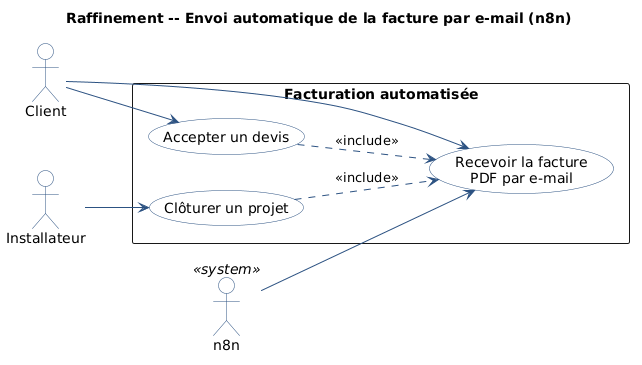
\includegraphics[width=0.92\textwidth]{uc-n8n-facture.png}%
  }{%
    \fbox{\parbox[c][7cm][c]{0.92\textwidth}{\centering
      Compiler \texttt{uc-n8n-facture.puml} $\rightarrow$ \texttt{uc-n8n-facture.png}%
    }}%
  }
  \caption{Diagramme de cas d'utilisation --- envoi automatique facture via n8n}
  \label{fig:uc-n8n-facture}
\end{figure}

\paragraph{Diagramme de séquence.}
La figure~\ref{fig:seq-n8n-facture} détaille les interactions entre le
\texttt{project-service}, n8n, l'endpoint interne PDF et le serveur SMTP
lors de l'acceptation d'un devis (déclencheur principal du sprint~5).

\begin{figure}[H]
  \centering
  \IfFileExists{seq-n8n-facture.png}{%
    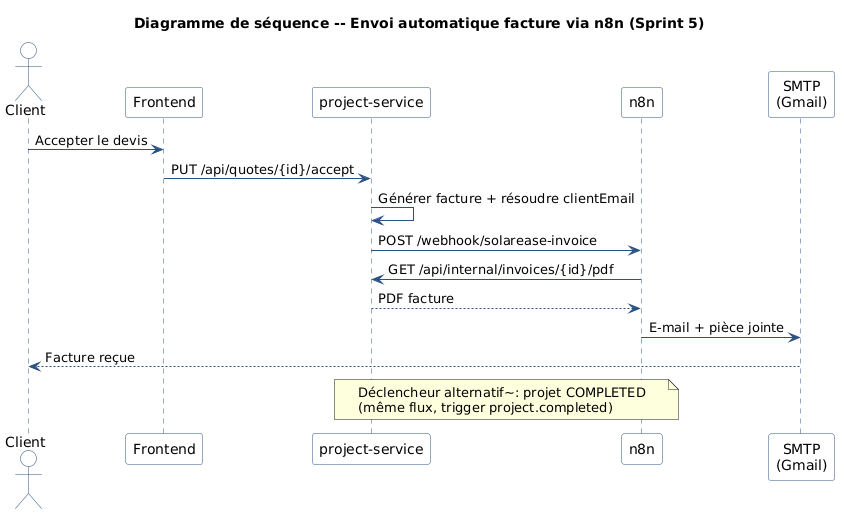
\includegraphics[width=0.95\textwidth]{seq-n8n-facture.png}%
  }{%
    \fbox{\parbox[c][8cm][c]{0.95\textwidth}{\centering
      Compiler \texttt{seq-n8n-facture.puml} $\rightarrow$ \texttt{seq-n8n-facture.png}%
    }}%
  }
  \caption{Diagramme de séquence --- workflow n8n d'envoi de facture PDF}
  \label{fig:seq-n8n-facture}
\end{figure}

\paragraph{Chaîne technique.}
Le flux comporte quatre étapes principales~:
(1)~après \texttt{generateInvoiceFromQuote()} ou passage en
\texttt{COMPLETED}, le \texttt{project-service} envoie un POST JSON au webhook
\texttt{/webhook/solarease-invoice}~;
(2)~n8n vérifie que \texttt{clientEmail} est renseigné~;
(3)~n8n récupère le PDF via
\texttt{GET /api/internal/invoices/\{id\}/pdf} (endpoint interne protégé par
\texttt{X-Internal-Secret}, sans JWT, accessible uniquement sur le réseau
Docker)~;
(4)~n8n envoie l'e-mail via SMTP (Gmail, port~587, STARTTLS) avec la facture
en pièce jointe.

\paragraph{Implémentation.}
Les composants principaux sont~:
\begin{itemize}[leftmargin=*, nosep]
  \item \texttt{N8nInvoiceWebhookService.java}~: construction du payload et
        appel HTTP vers n8n~;
  \item \texttt{InternalInvoiceController.java}~: téléchargement sécurisé du
        PDF pour n8n~;
  \item \texttt{backend/n8n/workflows/send-invoice-email.json}~: workflow
        versionné (webhook, condition e-mail, HTTP Request, envoi SMTP).
\end{itemize}

Le couplage reste faible~: le contrat JSON entre backend et n8n permet
d'ajouter ultérieurement d'autres automatisations (relance impayée,
notification Slack) sans modifier le cœur métier Java.

% ──────────────────────────────────────────────
\paragraph{Raffinement de cas d'utilisation «~Tableau de bord client~»}

\begin{figure}[H]
  \centering
  \IfFileExists{uc-client-dashboard.png}{%
    \includegraphics[width=0.85\textwidth]{uc-client-dashboard.png}%
  }{%
    \fbox{\parbox[c][6cm][c]{0.85\textwidth}{\centering Diagramme de cas d'utilisation -- Tableau de bord client}}%
  }
  \caption{Diagramme de cas d'utilisation pour «~Tableau de bord client~»}
  \label{fig:uc-dashboard-client}
\end{figure}

\subparagraph{Description textuelle du cas d'utilisation «~Consulter le tableau de bord client~»}

\begin{table}[H]
  \caption{Description textuelle du cas d'utilisation «~Consulter le tableau de bord client~»}
  \label{tab:cu-dashboard-client}
  \centering
  \begin{tabularx}{\textwidth}{|L{3.8cm}|X|}
    \hline
    \rowcolor{figblue!10}
    \textbf{Cas d'utilisation} & Consulter le tableau de bord client. \\
    \hline
    \textbf{Acteur initiateur} & Client authentifié \\
    \hline
    \textbf{But du cas} & Permettre au client de disposer d'une vue synthétique unique sur son projet~: progression, devis, factures, documents, messages et notifications. \\
    \hline
    \textbf{Précondition} & Le client est authentifié et possède au moins un projet associé. \\
    \hline
    \textbf{Description du scénario} &
    \textbf{Scénario principal :}\newline
    1. Le client se connecte à son espace.\newline
    2. Le frontend envoie \texttt{GET /api/clients/me/dashboard}.\newline
    3. Le service agrège en parallèle~: projets actifs, devis, factures, notifications non lues.\newline
    4. Le système construit un \texttt{DashboardClientResponse}.\newline
    5. L'écran affiche des cartes KPI, le stepper du projet actif, les liens rapides et les notifications récentes.\\
    \hline
    \textbf{Scénarios alternatifs} &
    \textit{Scénario alternatif 1 -- Aucun projet :}\newline
    \hspace*{6pt}3.1.~Un message d'accueil et un lien vers «~Mes demandes~» sont affichés.\\
    \hline
  \end{tabularx}
\end{table}

\subparagraph{Description textuelle du cas d'utilisation «~Suivre l'avancement du projet~»}

\begin{table}[H]
  \caption{Description textuelle du cas d'utilisation «~Suivre l'avancement du projet~»}
  \label{tab:cu-suivre-projet}
  \centering
  \begin{tabularx}{\textwidth}{|L{3.8cm}|X|}
    \hline
    \rowcolor{figblue!10}
    \textbf{Cas d'utilisation} & Suivre l'avancement de son projet. \\
    \hline
    \textbf{Acteur initiateur} & Client authentifié \\
    \hline
    \textbf{But du cas} & Permettre au client de visualiser la progression de son installation grâce à un \textit{stepper} 5 étapes et au pourcentage d'avancement temps réel remonté par l'installateur. \\
    \hline
    \textbf{Précondition} & Le client est authentifié et son projet est en cours. \\
    \hline
    \textbf{Description du scénario} &
    \textbf{Scénario principal :}\newline
    1. Le client clique sur sa carte projet depuis le dashboard.\newline
    2. Le frontend envoie \texttt{GET /api/projects/\{id\}}.\newline
    3. L'écran affiche un stepper en 5 étapes~: Étude $\rightarrow$ Validation $\rightarrow$ Installation $\rightarrow$ Mise en service $\rightarrow$ Terminé.\newline
    4. Le pourcentage d'avancement (\texttt{currentProgress}) est affiché avec une barre.\newline
    5. Les avancements terrain de l'installateur s'affichent dans une chronologie.\\
    \hline
    \textbf{Scénarios alternatifs} &
    \textit{Scénario alternatif 1 -- Projet annulé :}\newline
    \hspace*{6pt}3.1.~Un bandeau signale le statut \texttt{CANCELLED}.\\
    \hline
  \end{tabularx}
\end{table}

\subsection{Conception du sprint 5}

L'analyse conceptuelle de ce cinquième sprint comprendra la description des
diagrammes de séquence liés aux fonctionnalités majeures du sprint~5. Elle
se conclura par l'élaboration du diagramme de classes, synthétisant
l'ensemble des éléments étudiés.

\subsubsection{Diagrammes de séquence}

Dans cette phase, nous présentons les diagrammes de séquence correspondant
aux principales fonctionnalités développées lors du sprint~5. Ces diagrammes
illustrent les interactions entre les différents composants du système pour
chaque fonctionnalité ciblée.

% ──────────────────────────────────────────────
\paragraph{Diagramme de séquence «~Soumettre une demande solaire~»}

La figure ci-après présente le flux complet d'une demande solaire~:
soumission via le formulaire public, persistance, notification aux admins
et traitement (conversion en projet, demande de compléments ou rejet).

\begin{figure}[H]
  \centering
  \IfFileExists{seq-demande-solaire.png}{%
    \includegraphics[width=0.95\textwidth,height=0.75\textheight,keepaspectratio]{seq-demande-solaire.png}%
  }{%
    \fbox{\parbox[c][7cm][c]{0.92\textwidth}{\centering Diagramme de séquence «~Soumettre une demande solaire~»}}%
  }
  \caption{Diagramme de séquence «~Soumettre une demande solaire~»}
  \label{fig:seq-s5-demande}
\end{figure}

% ──────────────────────────────────────────────
\paragraph{Diagramme de séquence «~Cycle complet du devis~»}

La figure ci-après illustre le cycle de vie du devis~: création (\texttt{DRAFT}),
envoi au client (\texttt{SENT}), acceptation (\texttt{ACCEPTED}) et émission
automatique de la facture (\texttt{INVOICED}).

\begin{figure}[H]
  \centering
  \IfFileExists{seq-cycle-devis.png}{%
    \includegraphics[width=0.95\textwidth,height=0.75\textheight,keepaspectratio]{seq-cycle-devis.png}%
  }{%
    \fbox{\parbox[c][7cm][c]{0.92\textwidth}{\centering Diagramme de séquence «~Cycle complet du devis~»}}%
  }
  \caption{Diagramme de séquence «~Cycle complet du devis~»}
  \label{fig:seq-s5-quote}
\end{figure}

% ──────────────────────────────────────────────
\paragraph{Diagramme de séquence «~Consulter le tableau de bord client~»}

La figure ci-après détaille l'agrégation parallèle des données du dashboard
client~: projets actifs, devis, factures et notifications.

\begin{figure}[H]
  \centering
  \IfFileExists{seq-dashboard-client.png}{%
    \includegraphics[width=0.95\textwidth,height=0.7\textheight,keepaspectratio]{seq-dashboard-client.png}%
  }{%
    \fbox{\parbox[c][7cm][c]{0.92\textwidth}{\centering Diagramme de séquence «~Consulter le tableau de bord client~»}}%
  }
  \caption{Diagramme de séquence «~Consulter le tableau de bord client~»}
  \label{fig:seq-s5-dashboard}
\end{figure}

\subsubsection{Diagramme de classes du sprint 5}

Ce diagramme de classes global illustre l'architecture du projet, avec les
classes liées au sprint~5.

Il permet d'identifier clairement les entités utilisées lors de ce cinquième
sprint.

\begin{figure}[H]
  \centering
  \IfFileExists{class-sprint5.png}{%
    \includegraphics[width=0.85\textwidth]{class-sprint5.png}%
  }{%
    \fbox{\parbox[c][8cm][c]{0.92\textwidth}{\centering Diagramme de classes global du sprint 5}}%
  }
  \caption{Diagramme de classes global du sprint~5}
  \label{fig:class-s5}
\end{figure}

\subsection{Réalisation du sprint 5}

\subsubsection{Extraits de code significatifs}

\begin{lstlisting}[caption={QuoteService.java --- Acceptation et facturation automatique},
                   label=lst:quote-accept, language=Java]
@Service @Transactional @RequiredArgsConstructor
public class QuoteService {

    public QuoteDTO acceptQuote(Long quoteId) {
        QuoteEntity q = quoteRepository.findById(quoteId)
            .orElseThrow(() -> new ResourceNotFoundException("Quote not found"));
        if (q.getValidUntil() != null
            && q.getValidUntil().isBefore(LocalDate.now())) {
            throw new IllegalStateException("Quote has expired");
        }
        q.setStatus(QuoteEntity.QuoteStatus.ACCEPTED);
        q.setAcceptedAt(LocalDateTime.now());
        quoteRepository.save(q);

        // Auto-generate invoice
        InvoiceEntity invoice = generateInvoiceFromQuote(q);
        q.setStatus(QuoteEntity.QuoteStatus.INVOICED);
        quoteRepository.save(q);

        // Notify installer and client
        notificationService.notifyQuoteAccepted(q);
        notificationService.notifyInvoiceGenerated(invoice);
        return mapToDTO(q);
    }

    private InvoiceEntity generateInvoiceFromQuote(QuoteEntity q) {
        InvoiceEntity inv = InvoiceEntity.builder()
            .number("INV-" + java.time.Year.now() + "-"
                + String.format("%05d", new Random().nextInt(99999)))
            .project(q.getProject()).clientId(q.getClientId())
            .installerId(q.getInstallerId())
            .amount(q.getTotalAmount()).status("SENT")
            .date(LocalDate.now())
            .dueDate(LocalDate.now().plusDays(30))
            .quoteId(q.getId()).build();
        return invoiceRepository.save(inv);
    }
}
\end{lstlisting}

\begin{lstlisting}[caption={AccessControlService.java --- Contrôle d'accès multi-rôle},
                   label=lst:access-ctrl, language=Java]
@Service
public class AccessControlService {

    public void requireAnyRole(String userRole, String... allowedRoles) {
        boolean allowed = Arrays.stream(allowedRoles)
            .anyMatch(r -> r.equalsIgnoreCase(userRole));
        if (!allowed) {
            throw new AuthorizationException(
                "Role " + userRole + " is not authorized");
        }
    }

    public void requireClientOwnsResource(String userRole,
            String userId, String resourceClientId) {
        if ("CLIENT".equalsIgnoreCase(userRole)
            && !userId.equals(resourceClientId)) {
            throw new AuthorizationException("Access denied");
        }
    }
}
\end{lstlisting}

\subsubsection{Interfaces utilisateur réalisées}

\begin{figure}[H]
  \centering
  \fbox{\parbox{0.85\textwidth}{
    \centering\vspace{0.5cm}
    \textit{Tableau de bord de l'espace client}\\[4pt]
    \small Remplacer par : \texttt{\textbackslash includegraphics[width=0.85\textbackslash textwidth]\{images/client-dashboard.png\}}\\[4pt]
    KPI (projets actifs, terminés, notifs), projet actif avec barre de progression, liens rapides
    \vspace{0.5cm}
  }}
  \caption{Tableau de bord client -- Sprint 5}
  \label{fig:ui-client-dashboard}
\end{figure}

\begin{figure}[H]
  \centering
  \fbox{\parbox{0.85\textwidth}{
    \centering\vspace{0.5cm}
    \textit{Détail du projet côté client avec stepper et avancement}\\[4pt]
    \small Remplacer par : \texttt{\textbackslash includegraphics[width=0.85\textbackslash textwidth]\{images/client-project-detail.png\}}\\[4pt]
    Stepper 5 étapes (Étude, Validation, Installation, Mise en service, Terminé), barre avancement terrain, devis
    \vspace{0.5cm}
  }}
  \caption{Détail projet espace client avec stepper -- Sprint 5}
  \label{fig:ui-client-detail}
\end{figure}

\begin{figure}[H]
  \centering
  \fbox{\parbox{0.85\textwidth}{
    \centering\vspace{0.5cm}
    \textit{Interface de gestion des devis}\\[4pt]
    \small Remplacer par : \texttt{\textbackslash includegraphics[width=0.85\textbackslash textwidth]\{images/quotes-list.png\}}\\[4pt]
    Liste des devis avec statut (DRAFT, SENT, ACCEPTED, INVOICED), actions contextuelles
    \vspace{0.5cm}
  }}
  \caption{Gestion des devis -- Sprint 5}
  \label{fig:ui-quotes}
\end{figure}

\begin{figure}[H]
  \centering
  \fbox{\parbox{0.85\textwidth}{
    \centering\vspace{0.5cm}
    \textit{Acceptation de devis côté client}\\[4pt]
    \small Remplacer par : \texttt{\textbackslash includegraphics[width=0.85\textbackslash textwidth]\{images/quote-accept.png\}}\\[4pt]
    Carte devis avec détails (main-d'œuvre, matériaux, TVA, total), boutons Accepter / Refuser
    \vspace{0.5cm}
  }}
  \caption{Acceptation de devis par le client -- Sprint 5}
  \label{fig:ui-quote-accept}
\end{figure}

\begin{figure}[H]
  \centering
  \fbox{\parbox{0.85\textwidth}{
    \centering\vspace{0.5cm}
    \textit{Gestion des demandes solaires (côté admin)}\\[4pt]
    \small Remplacer par : \texttt{\textbackslash includegraphics[width=0.85\textbackslash textwidth]\{images/demands-admin.png\}}\\[4pt]
    Liste des demandes avec filtres par statut, actions : compléter, valider, convertir en projet
    \vspace{0.5cm}
  }}
  \caption{Gestion des demandes solaires -- Sprint 5}
  \label{fig:ui-demands}
\end{figure}

\begin{figure}[H]
  \centering
  \fbox{\parbox{0.85\textwidth}{
    \centering\vspace{0.5cm}
    \textit{Liste des factures avec téléchargement PDF}\\[4pt]
    \small Remplacer par : \texttt{\textbackslash includegraphics[width=0.85\textbackslash textwidth]\{images/invoices-list.png\}}\\[4pt]
    Factures auto-générées, numéro INV-2026-XXXXX, statut (DRAFT, SENT, PAID), bouton PDF
    \vspace{0.5cm}
  }}
  \caption{Liste des factures -- Sprint 5}
  \label{fig:ui-invoices}
\end{figure}

\subsection{Environnement des sprints 4 et 5}

\begin{table}[H]
  \caption{Technologies et outils utilisés -- Sprints 4 et 5}
  \label{tab:tech-r3}
  \centering
  \begin{tabularx}{\textwidth}{|L{3cm}|L{3cm}|X|}
    \hline
    \rowcolor{figblue!20}
    \textbf{Technologie} & \textbf{Version} & \textbf{Rôle dans les sprints 4 et 5} \\
    \hline
    Spring WebSocket & 3.2 & Communication temps réel STOMP/SockJS \\
    \hline
    SockJS & 1.x & Fallback WebSocket pour navigateurs incompatibles \\
    \hline
    STOMP & 1.2 & Protocole de messagerie sur WebSocket \\
    \hline
    OpenPDF & 1.3.x & Génération des factures PDF \\
    \hline
    JavaMail & -- & Envoi d'emails d'invitation et notification \\
    \hline
    Twilio & -- & Envoi de SMS d'invitation (stub) \\
    \hline
    Flyway & 10.x & Migrations V1--V12 (devis, factures, demandes, conversations, etc.) \\
    \hline
    React & 18.x & Espace client~: dashboard, stepper, cartes devis \\
    \hline
    Framer Motion & 11.x & Animations du stepper et des transitions de page \\
    \hline
    Sonner & 1.x & Toasts de notification côté frontend \\
    \hline
  \end{tabularx}
\end{table}

\subsubsection{Tests et validation}

\begin{table}[H]
  \caption{Résultats des tests fonctionnels -- Sprint 5}
  \label{tab:tests-s5}
  \centering\small
  \begin{tabularx}{\textwidth}{|C{1.2cm}|L{3.5cm}|X|C{1.4cm}|}
    \hline
    \rowcolor{figblue!20}
    \textbf{ID} & \textbf{Cas de test} & \textbf{Résultat attendu} & \textbf{Statut} \\
    \hline
    T-34 & Demande publique & HTTP 201, statut NOUVELLE & \ok~OK \\
    \hline
    T-35 & Conversion demande & Projet créé, demande VALIDEE & \ok~OK \\
    \hline
    T-36 & Créer devis DRAFT & HTTP 201, numéro auto-généré & \ok~OK \\
    \hline
    T-37 & Envoyer devis & DRAFT$\to$SENT, client notifié & \ok~OK \\
    \hline
    T-38 & Accepter devis & SENT$\to$ACCEPTED$\to$INVOICED, facture créée & \ok~OK \\
    \hline
    T-39 & Refuser devis & SENT$\to$REJECTED, raison enregistrée & \ok~OK \\
    \hline
    T-40 & Devis expiré & Acceptation refusée, HTTP 400 & \ok~OK \\
    \hline
    T-41 & Facture PDF & PDF valide généré, téléchargement OK & \ok~OK \\
    \hline
    T-47 & Envoi n8n facture & Webhook OK, e-mail reçu à \texttt{clientEmail} & \ok~OK \\
    \hline
    T-42 & Dashboard client & KPI affichés, projet actif en avant & \ok~OK \\
    \hline
    T-43 & Stepper client & Progression synchronisée avec statut & \ok~OK \\
    \hline
    T-44 & Accès non autorisé & HTTP 403, client ne voit que ses données & \ok~OK \\
    \hline
    T-45 & CRUD installateurs & Création, modification, suppression admin & \ok~OK \\
    \hline
    T-46 & Invitation client & Email envoyé avec lien d'inscription & \ok~OK \\
    \hline
  \end{tabularx}
\end{table}

\begin{conclusionbox}
Les sprints 3, 4 et 5 finalisent la plateforme SolarEase en la dotant de toutes les
fonctionnalités nécessaires à une exploitation opérationnelle. Le suivi
terrain temps réel permet à l'installateur de communiquer son avancement
depuis le chantier. La messagerie et les notifications assurent une
collaboration fluide entre les trois rôles (admin, installateur, client).
L'espace client offre une expérience dédiée avec un suivi visuel du projet
à travers un stepper intuitif. Enfin, le workflow commercial complet ---
de la demande solaire à la facturation automatique en passant par le devis,
puis l'envoi de la facture PDF par e-mail via n8n (section~\ref{sec:n8n}) ---
transforme SolarEase en une solution professionnelle de gestion de projets
solaires, prête pour le marché tunisien.
\end{conclusionbox}

\cleardoublepage


\chapterpage{5}{DevOps et mise en production}
% ============================================================
%  12-devops.tex
%  Chapitre 5 : DevOps et mise en production
%
%  Captures à placer dans rapport/overleaf/images/devops/ :
%    actions.png             -> GitHub > Actions (liste workflows)
%    docker-azure.png        -> SSH : docker compose ps
%    deploy-success.png      -> Actions > Deploy (run vert)
%    actuator-health.png     -> curl ou navigateur /actuator/health UP
%    grafana-dashboard.png   -> Grafana :3000 (si observability lancée)
%    vercel-login.png        -> https://solar-ease-sxyy.vercel.app/login OK
%  Schéma : devops.png -> Chaîne DevOps et déploiement
% ============================================================

\newcommand{\devopsfig}[4][0.88]{%
  \begin{figure}[H]
    \centering
    \IfFileExists{#2}{%
      \includegraphics[width=#1\textwidth]{#2}%
    }{%
      \fbox{\parbox[c][4cm][c]{#1\textwidth}{\centering
        \small\textit{Capture à ajouter}\\[4pt]
        \small\texttt{#2}\\[4pt]
        \small #3
      }}%
    }
    \caption{#4}
  \end{figure}
}

\chapter{DevOps et mise en production}

\begin{chapterintro}
Ce chapitre présente l'industrialisation de SolarEase~: containerisation,
CI/CD GitHub Actions, observabilité, sécurité, puis la \textbf{mise en
production réelle} (frontend Vercel, backend sur VM Azure). L'objectif est
de garantir des livraisons reproductibles, traçables et vérifiables~: chaque
\textit{push} déclenche des contrôles automatisés, le déploiement backend
s'effectue par SSH sans intervention manuelle sur la VM, et les figures
illustrent la chaîne DevOps ainsi que les preuves de bon fonctionnement en
production (captures d'écran).
\end{chapterintro}

% ══════════════════════════════════════════════════════════
\section{Architecture et principes}
% ══════════════════════════════════════════════════════════

La démarche s'appuie sur le cadre \textbf{CALMS}~:
\textbf{C}ulture (intégration continue partagée par l'équipe)~;
\textbf{A}utomation (workflows GitHub Actions)~;
\textbf{L}ean (pipelines courts, retour rapide)~;
\textbf{M}easurement (Prometheus, Grafana, health checks)~;
\textbf{S}haring (Docker Compose, manifests K8s, \texttt{RUNBOOK.md}).

Concrètement, le cycle de vie suit trois axes~: (1)~développement local
via Vite + Compose~; (2)~intégration continue à chaque \textit{push} ou PR
(build Maven, tests, scans)~; (3)~déploiement de démonstration sur Azure
et Vercel, avec vérification post-déploiement (\texttt{/actuator/health}).

\devopsfig[0.95]{devops.png}{Ajouter \texttt{devops.png}.}{Chaîne DevOps et déploiement de démonstration}

% ══════════════════════════════════════════════════════════
\section{Containerisation}
% ══════════════════════════════════════════════════════════

Chaque microservice utilise un \texttt{Dockerfile} \textbf{multi-stage}~:
une étape \texttt{build} (Maven~3.9, Temurin~17) compile le JAR, une étape
\texttt{runtime} embarque uniquement le JAR sur une image JRE Alpine (ou
Debian pour \texttt{dimensioning-service}, avec Tesseract OCR pour l'extraction
de factures). Cette séparation réduit la taille des images et la surface
d'attaque.

Le fichier \texttt{backend/docker-compose.yml} orchestre l'ensemble sur le
réseau bridge \texttt{solarease-net}~:
\begin{itemize}[leftmargin=*, nosep]
  \item \textbf{Gateway} (8080)~: point d'entrée unique, routage JWT~;
  \item \textbf{Identity} (8081), \textbf{Project} (8082),
        \textbf{Dimensioning} (8083)~: microservices métier~;
  \item trois instances \textbf{PostgreSQL~16} (identity, project,
        dimensioning avec \texttt{pgvector})~;
  \item \textbf{Ollama} et \textbf{n8n} pour l'assistant IA et l'automatisation.
\end{itemize}

En local, le frontend Vite (\texttt{npm run dev}, port~5173) appelle
\texttt{/api} via le proxy Vite~; en production, c'est \texttt{vercel.json}
qui assure le même rôle (voir section~\ref{sec:prod-pfe}).

\devopsfig{docker-azure.png}{Terminal SSH sur la VM Azure~:
\texttt{cd \textasciitilde/SolarEase/backend \&\& docker compose ps}.}
{Stack Docker en production sur la VM Azure -- neuf conteneurs actifs}

% ══════════════════════════════════════════════════════════
\section{Pipeline CI/CD}
% ══════════════════════════════════════════════════════════

Quatre workflows GitHub Actions couvrent le cycle de livraison. Ils sont
déclenchés de façon \textbf{ciblée} (\texttt{paths}) afin d'éviter des runs
inutiles lors de modifications du rapport ou du frontend seul.

\begin{table}[H]
  \caption{Workflows GitHub Actions}
  \label{tab:workflows}
  \centering\small
  \begin{tabularx}{\textwidth}{|L{3.8cm}|L{4cm}|X|}
    \hline
    \rowcolor{black!12}
    \textbf{Fichier} & \textbf{Déclencheur} & \textbf{Rôle} \\
    \hline
    \texttt{backend-ci.yml} & push/PR \texttt{backend/**} &
    \texttt{mvn verify} en matrice (4 services), JaCoCo \\
    \hline
    \texttt{docker-publish.yml} & \texttt{main}, tags \texttt{v*} &
    Build et push images sur GHCR \\
    \hline
    \texttt{security-scan.yml} & push, PR, cron &
    Trivy (fs + images), Gitleaks \\
    \hline
    \texttt{deploy.yml} & push \texttt{main}, manuel &
    Déploiement VM Azure (SSH, \texttt{docker compose up}) \\
    \hline
  \end{tabularx}
\end{table}

Le workflow \texttt{deploy.yml} s'exécute via \texttt{appleboy/ssh-action}~:
connexion à la VM avec les secrets \texttt{AZURE} (IP), \texttt{AZURE\_VM}
(utilisateur) et \texttt{AZURE\_VM\_SSH\_KEY} (clé privée)~; puis
\texttt{git pull}, \texttt{docker compose up -d --build}, et boucle d'attente
sur \texttt{/actuator/health} (jusqu'à 3~minutes) avant de valider le déploiement.

\devopsfig{actions.png}{GitHub $\rightarrow$ SolarEase
$\rightarrow$ Actions. Montrer Backend CI, Deploy, Docker Publish,
Security Scan.}{Interface GitHub Actions -- workflows automatisés}

\devopsfig{devops2.png}{Actions $\rightarrow$ Deploy
$\rightarrow$ run réussi (coche verte).}{Workflow Deploy -- mise à jour
automatisée du backend sur Azure}

% ══════════════════════════════════════════════════════════
\section{Observabilité}
% ══════════════════════════════════════════════════════════

Chaque microservice Spring Boot expose \texttt{/actuator/health} (sonde de
vivacité) et \texttt{/actuator/prometheus} (métriques Micrometer). La stack
optionnelle est décrite dans
\texttt{backend/observability/docker-compose.observability.yml} et se lance
en complément du Compose principal~:

\begin{itemize}[leftmargin=*, nosep]
  \item \textbf{Prometheus} (9090)~: scrape toutes les 15~s les quatre
        services sur le réseau Docker~;
  \item \textbf{Grafana} (3000)~: dashboards provisionnés
        (\texttt{solarease.json}), sources Prometheus et Loki auto-configurées~;
  \item \textbf{Loki} (3100) + \textbf{Promtail}~: centralisation des logs
        conteneurs via le socket Docker.
\end{itemize}

Un correctif PFE a aligné les chemins \texttt{observability/} et la config
Loki (\texttt{ring.kvstore: inmemory}) pour un démarrage fiable sur VM à
ressources limitées. L'accès Grafana en production se fait via tunnel SSH
(port~3000 non exposé publiquement) ou en local après
\texttt{docker compose -f \ldots observability.yml up -d}.

\devopsfig{devops5.png}{Démarrer la stack
observability puis ouvrir \texttt{localhost:3000} ou l'IP VM :3000.}
{Dashboard Grafana -- métriques des microservices}

% ══════════════════════════════════════════════════════════
\section{Qualité et sécurité}
% ══════════════════════════════════════════════════════════

\textbf{JaCoCo} génère la couverture de code à l'étape \texttt{mvn verify}~;
\textbf{Trivy} analyse le système de fichiers et les images Docker~;
\textbf{Gitleaks} détecte les fuites de secrets dans l'historique Git.
Les résultats Trivy/Gitleaks sont publiés en \textbf{SARIF} pour consultation
dans l'onglet \textit{Security} de GitHub.

Les secrets applicatifs et d'infrastructure restent \textbf{hors Git}~:
fichier \texttt{backend/.env} (non versionné), secrets GitHub Actions pour
Azure et variables Vercel pour le frontend. Aucune clé SSH ni mot de passe
n'apparaît dans le dépôt~; la clé de déploiement est stockée chiffrée côté
GitHub et la clé publique correspondante dans
\texttt{\textasciitilde/.ssh/authorized\_keys} sur la VM.

% ══════════════════════════════════════════════════════════
\section{Mise en production (démo PFE)}
% ══════════════════════════════════════════════════════════
\label{sec:prod-pfe}

Le \textbf{backend} tourne sur une \textbf{VM Azure} (Ubuntu~24.04,
France Central, IP publique \texttt{4.233.29.236})~; le \textbf{frontend}
React/Vite est hébergé sur \textbf{Vercel}
(\url{https://solar-ease-sxyy.vercel.app}).

\paragraph{Déploiement backend.}
Clone du dépôt GitHub sur la VM (\texttt{\textasciitilde/SolarEase}),
\texttt{docker compose up -d --build}, NSG Azure avec la règle TCP~8080
ouverte. Le workflow \texttt{deploy.yml} automatise cette séquence à chaque
\textit{push} sur \texttt{main} modifiant \texttt{backend/**}.

\paragraph{Déploiement frontend.}
Vercel build le dossier frontend (\texttt{npm run build}, sortie \texttt{dist}).
Le fichier \texttt{vercel.json} réécrit \texttt{/api/:path*} et \texttt{/ws}
vers le gateway Azure, sans variable \texttt{VITE\_API\_URL} en production~:
le navigateur appelle le même domaine Vercel, qui proxifie vers la VM. Ainsi,
l'authentification JWT transite par \texttt{POST /api/auth/login} sur
\texttt{solar-ease-sxyy.vercel.app}, preuve que la chaîne frontend $\rightarrow$
rewrite $\rightarrow$ gateway $\rightarrow$ identity-service fonctionne de bout
en bout.

\devopsfig{devops8.png}{Navigateur ou terminal~:
\texttt{http://4.233.29.236:8080/actuator/health} avec statut UP.}
{Health check public du gateway Azure}

\devopsfig{devops10.png}{URL production Vercel, login
admin réussi (\texttt{admin@solarease.demo}).}{Application SolarEase en
production -- authentification via rewrite Vercel}

\begin{table}[H]
  \caption{Environnements SolarEase}
  \label{tab:environments}
  \centering\small
  \begin{tabularx}{\textwidth}{|L{2.2cm}|L{3.2cm}|L{3.5cm}|X|}
    \hline
    \rowcolor{black!12}
    \textbf{Env.} & \textbf{Backend} & \textbf{Frontend} & \textbf{Usage} \\
    \hline
    Local & Docker Compose & \texttt{npm run dev} & Développement \\
    \hline
    Production & VM Azure + Compose & Vercel & Démo PFE, URL publique \\
    \hline
  \end{tabularx}
\end{table}

% ══════════════════════════════════════════════════════════
\section{Infrastructure as Code (Kubernetes)}
% ══════════════════════════════════════════════════════════

Le dossier \texttt{k8s/} (Kustomize, overlays \texttt{dev}/\texttt{prod})
documente une montée en charge cloud-native~: Deployments par microservice,
Services ClusterIP, ConfigMaps et Secrets. Cette voie n'est pas activée pour
la démo PFE (coût et complexité), mais permet une évolution future via
\texttt{kubectl apply -k k8s/overlays/prod} sans réécrire les manifests.

% ══════════════════════════════════════════════════════════
\section{Tests de validation}
% ══════════════════════════════════════════════════════════

Les scénarios ci-dessous ont été exécutés manuellement ou via CI pour valider
la chaîne DevOps et la mise en production.

\begin{table}[H]
  \caption{Validation DevOps (extrait)}
  \label{tab:devops-tests}
  \centering\small
  \begin{tabularx}{\textwidth}{|C{1cm}|L{4.2cm}|X|C{1.2cm}|}
    \hline
    \rowcolor{black!12}
    \textbf{ID} & \textbf{Test} & \textbf{Résultat attendu} & \textbf{Statut} \\
    \hline
    D-01 & \texttt{docker compose up} & Stack UP $<$60s & \ok~OK \\
    \hline
    D-02 & PR sur backend & CI verte (4 services) & \ok~OK \\
    \hline
    D-03 & \texttt{deploy.yml} sur \texttt{main} & SSH + health UP & \ok~OK \\
    \hline
    D-07 & Logs $\rightarrow$ Loki & Filtre par conteneur & \ok~OK \\
    \hline
    D-13 & Health gateway Azure & \texttt{UP} sur :8080 & \ok~OK \\
    \hline
    D-14 & Login via Vercel & Auth OK via \texttt{/api} & \ok~OK \\
    \hline
  \end{tabularx}
\end{table}

\begin{conclusionbox}
SolarEase dispose d'une chaîne DevOps complète (build, tests, scans,
observabilité) et d'une mise en production opérationnelle Vercel + Azure.
Les captures d'écran du chapitre --- stack Docker sur VM, workflows Actions,
health check public, dashboard Grafana et login production --- constituent
les preuves visuelles de cette industrialisation et du critère D-14
(authentification bout en bout via rewrite).
\end{conclusionbox}


% ── Conclusion générale ─────────────────────────────────────
% ============================================================
%  13-conclusion.tex  —  Conclusion générale et perspectives
% ============================================================
\chapterstar{Conclusion Générale et Perspectives}

\begin{chapterintro}
  Ce chapitre clôture le rapport en synthétisant les réalisations du projet
  SolarEase, en dressant un bilan critique et en exposant les perspectives
  d'évolution à court et moyen terme.
\end{chapterintro}

\section*{Synthèse des réalisations}

Le projet \textbf{SolarEase} a permis de concevoir et de réaliser une
plateforme web complète répondant aux besoins des sociétés d'installation
de panneaux solaires. Organisé en sprints Kanban successifs, le travail
accompli couvre~:

\begin{itemize}
  \item \textbf{Chapitre~3 (Sprints 1 et 2)~:} socle technique et gestion
    métier~: authentification sécurisée (inscription client OTP, comptes
    installateurs par l'admin, JWT, Gateway), gestion des clients et
    projets (CRUD, cycle de vie 6 statuts, tableau de bord KPI)~;
  \item \textbf{Chapitre~4 (Sprints 3, 4 et 5)~:} cœur métier et
    collaboration~: moteur de dimensionnement photovoltaïque (données PVGIS
    réelles, modèle Night Panel, analyse financière sur 25 ans), approche
    RAG \textbf{hybride} pour les recommandations IA (sélection
    déterministe sur le catalogue société + base vectorielle
    \texttt{pgvector} + Ollama), génération automatique de rapports PDF
    professionnels, suivi terrain avec mises à jour de progression,
    messagerie temps réel (WebSocket), centre de notifications, espace
    client dédié avec stepper de suivi, gestion des demandes solaires,
    devis avec acceptation client et facturation automatique~;
  \item \textbf{DevOps (Chapitre~5)~:} industrialisation complète de la
    chaîne logicielle backend~: containerisation multi-stage des 4
    microservices, pipeline CI/CD GitHub Actions (build, tests, scans
    Trivy/Gitleaks, publication d'images sur GHCR), stack d'observabilité
    (Spring Actuator + Prometheus + Grafana + Loki), qualité (JaCoCo),
    Infrastructure as Code (Kubernetes + Kustomize, overlays dev/prod),
    déploiement automatique Railway sur les branches \texttt{develop} et
    les tags \texttt{v*.*.*}. Le frontend React/Vite reste un projet
    léger livré en continu sur Vercel.
\end{itemize}

\section*{Bilan des objectifs atteints}

\begin{table}[H]
  \caption{Bilan des objectifs du projet SolarEase}
  \label{tab:bilan}
  \centering
  \begin{tabularx}{\textwidth}{|L{5cm}|C{2cm}|X|}
    \hline
    \rowcolor{figblue}
    \textcolor{white}{\textbf{Objectif}} &
    \textcolor{white}{\textbf{Atteint}} &
    \textcolor{white}{\textbf{Commentaire}} \\
    \hline
    Authentification sécurisée JWT+OTP & \textcolor{green!70!black}{\checkmark} Oui & Entièrement fonctionnel \\
    \hline
    Gestion clients et projets & \textcolor{green!70!black}{\checkmark} Oui & CRUD + cycle de vie \\
    \hline
    Moteur de dimensionnement & \textcolor{green!70!black}{\checkmark} Oui & PVGIS + fallback \\
    \hline
    Innovation Night Panel & \textcolor{green!70!black}{\checkmark} Oui & Formules validées \\
    \hline
    Analyse financière 25 ans & \textcolor{green!70!black}{\checkmark} Oui & ROI, payback, cash-flow \\
    \hline
    Génération rapport PDF & \textcolor{green!70!black}{\checkmark} Oui & Téléchargement direct \\
    \hline
    Recommandation IA & \textcolor{green!70!black}{\checkmark} Oui & Ollama en fallback contrôlé \\
    \hline
    Architecture microservices & \textcolor{green!70!black}{\checkmark} Oui & 4 services + Docker Compose \\
    \hline
    Pipeline CI/CD automatisé & \textcolor{green!70!black}{\checkmark} Oui & GitHub Actions + GHCR \\
    \hline
    Observabilité (métriques + logs) & \textcolor{green!70!black}{\checkmark} Oui & Prometheus + Grafana + Loki \\
    \hline
    Infrastructure as Code & \textcolor{green!70!black}{\checkmark} Oui & Kustomize (base + overlays) \\
    \hline
    Déploiement multi-environnement & \textcolor{green!70!black}{\checkmark} Oui & Railway staging + prod \\
    \hline
  \end{tabularx}
\end{table}

\section*{Bilan critique}

\textbf{Points forts~:}
\begin{itemize}
  \item Architecture moderne, découplée et évolutive~;
  \item Données de production basées sur PVGIS (source officielle européenne)~;
  \item Innovation significative avec le mode Night~Panel et la couverture nocturne~;
  \item Expérience utilisateur professionnelle avec deux espaces distincts~;
  \item Résilience assurée par les mécanismes de fallback (PVGIS et IA).
\end{itemize}

\textbf{Limites identifiées~:}
\begin{itemize}
  \item Dépendance partielle à des services externes (PVGIS, Ollama)~;
  \item Paramètres de calibration (prix kWh, taux dégradation) à valider avec
    chaque société partenaire~;
  \item Absence de tests de charge exhaustifs en conditions de production.
\end{itemize}

\section*{Perspectives d'évolution}

À court terme~:
\begin{itemize}
  \item Intégration d'un \textbf{tableau de bord analytique avancé} avec
    visualisations des économies réalisées~;
  \item Enrichissement de la \textbf{base de connaissances IA} avec des
    données spécifiques au marché tunisien~;
  \item Ajout d'un \textbf{module de signature électronique} pour les devis.
\end{itemize}

À moyen terme~:
\begin{itemize}
  \item \textbf{Architecture multi-tenant} pour servir plusieurs sociétés
    d'installation depuis une même instance~;
  \item \textbf{Application mobile} React Native pour les commerciaux terrain~;
  \item Mise en place d'\textbf{Alertmanager} couplé à Slack/Teams pour les
    alertes critiques sur les métriques Prometheus déjà collectées~;
  \item Tests \textbf{end-to-end} automatisés (Playwright) intégrés au
    pipeline GitHub Actions~;
  \item Adoption d'un \textbf{service mesh} (Istio ou Linkerd) pour la
    résilience inter-services en production~;
  \item Connexion aux systèmes de \textbf{monitoring en temps réel} des
    installations existantes.
\end{itemize}

\vspace{0.8cm}
\begin{center}
  \begin{tcolorbox}[colback=isetblue!8, colframe=isetblue,
      width=0.9\textwidth, halign=center, fontupper=\itshape]
    SolarEase démontre qu'il est possible de développer, en solo, une
    plateforme professionnelle complète en appliquant rigoureusement les
    bonnes pratiques d'ingénierie logicielle~: architecture microservices,
    sécurité centralisée, tests automatisés et déploiement conteneurisé.
    Ce projet constitue une base solide et extensible pour une mise en
    production réelle dans le secteur des énergies renouvelables.
  \end{tcolorbox}
\end{center}

\cleardoublepage


% ── Bibliographie ───────────────────────────────────────────
% ============================================================
%  14-bibliographie.tex  —  Bibliographie & Netographie
% ============================================================
\chapterstar{Bibliographie et Netographie}

\section*{Ouvrages et articles}

\begin{enumerate}[label={[\arabic*]}]
  \item \textsc{Fowler}, M. (2018). \textit{Microservices Patterns}. Manning Publications.
  \item \textsc{Newman}, S. (2019). \textit{Building Microservices, 2nd edition}. O'Reilly Media.
  \item \textsc{Walls}, C. (2022). \textit{Spring Boot in Action}. Manning Publications.
  \item \textsc{Banks}, A. \& \textsc{Porcello}, E. (2020).
    \textit{Learning React, 2nd edition}. O'Reilly Media.
  \item \textsc{Kruchten}, P. (2004). \textit{The Rational Unified Process: An Introduction},
    Addison-Wesley.
  \item \textsc{Schwaber}, K. \& \textsc{Sutherland}, J. (2020).
    \textit{The Scrum Guide}. Scrum.org.
\end{enumerate}

\section*{Documentation technique}

\begin{enumerate}[label={[\arabic*]}, resume]
  \item Spring Boot Reference Documentation (3.2.x).
    \url{https://docs.spring.io/spring-boot/docs/3.2.x/reference/}
    [Consulté en mars 2026]
  \item Spring Security Reference Documentation.
    \url{https://docs.spring.io/spring-security/reference/}
    [Consulté en mars 2026]
  \item React Documentation.
    \url{https://react.dev}
    [Consulté en février 2026]
  \item PostgreSQL 16 Documentation.
    \url{https://www.postgresql.org/docs/16/}
    [Consulté en janvier 2026]
  \item Docker Compose Documentation.
    \url{https://docs.docker.com/compose/}
    [Consulté en janvier 2026]
\end{enumerate}

\section*{APIs et services externes}

\begin{enumerate}[label={[\arabic*]}, resume]
  \item PVGIS -- Commission Européenne. API de calcul photovoltaïque.
    \url{https://re.jrc.ec.europa.eu/pvg_tools/en/}
    [Consulté en février 2026]
  \item Ollama -- LLM local.
    \url{https://ollama.ai}
    [Consulté en mars 2026]
  \item TinyLLaMA -- Modèle de langage compact.
    \url{https://github.com/jzhang38/TinyLlama}
    [Consulté en mars 2026]
\end{enumerate}

\section*{Ressources ISET Nabeul}

\begin{enumerate}[label={[\arabic*]}, resume]
  \item Département Technologies de l'Informatique, ISET Nabeul.
    \textit{Guide de rédaction du rapport PFE -- Version 2023}.
  \item Référentiel de la Licence en Développement Systèmes d'Informations,
    ISET Nabeul, 2025/2026.
\end{enumerate}

\cleardoublepage


% ── Annexes ─────────────────────────────────────────────────
% ============================================================
%  15-annexes.tex  —  Annexes
% ============================================================
\appendix
\renewcommand{\chaptername}{Annexe}

% ── ANNEXE A ──────────────────────────────────────────────
\chapter{Récapitulatif Complet des Endpoints API}

\section*{A.1 Identity Service (Port 8081)}

\begin{table}[H]
  \caption{Endpoints Identity Service}
  \centering
  \begin{tabularx}{\textwidth}{|C{1.5cm}|L{5.5cm}|X|C{2cm}|}
    \hline
    \rowcolor{figblue}
    \textcolor{white}{\textbf{Méthode}} &
    \textcolor{white}{\textbf{Route}} &
    \textcolor{white}{\textbf{Description}} &
    \textcolor{white}{\textbf{Auth}} \\
    \hline
    POST & /api/auth/register & Inscription + OTP & Non \\
    \hline
    POST & /api/auth/verify-otp & Validation OTP & Non \\
    \hline
    POST & /api/auth/login & Connexion JWT & Non \\
    \hline
    POST & /api/auth/refresh & Refresh token & Non \\
    \hline
    POST & /api/auth/resend-otp & Renvoi OTP & Non \\
    \hline
    GET & /api/auth/me & Profil utilisateur & JWT \\
    \hline
    PUT & /api/auth/me & MAJ profil & JWT \\
    \hline
    PUT & /api/auth/me/password & Changement MD passe & JWT \\
    \hline
    GET & /api/auth/health & Health check & Non \\
    \hline
  \end{tabularx}
\end{table}

\section*{A.2 Project Service (Port 8082)}

\begin{table}[H]
  \caption{Endpoints Project Service}
  \centering
  \begin{tabularx}{\textwidth}{|C{1.5cm}|L{5.5cm}|X|C{2cm}|}
    \hline
    \rowcolor{figblue}
    \textcolor{white}{\textbf{Méthode}} &
    \textcolor{white}{\textbf{Route}} &
    \textcolor{white}{\textbf{Description}} &
    \textcolor{white}{\textbf{Auth}} \\
    \hline
    GET & /api/clients & Liste clients paginée & JWT \\
    \hline
    POST & /api/clients & Créer un client & JWT \\
    \hline
    GET & /api/clients/\{id\} & Détail client & JWT \\
    \hline
    PUT & /api/clients/\{id\} & Modifier client & JWT \\
    \hline
    DELETE & /api/clients/\{id\} & Supprimer client & JWT \\
    \hline
    GET & /api/projects & Liste projets & JWT \\
    \hline
    POST & /api/projects & Créer projet & JWT \\
    \hline
    GET & /api/projects/\{id\} & Détail projet & JWT \\
    \hline
    PATCH & /api/projects/\{id\}/status & Changer statut & JWT \\
    \hline
    GET & /api/projects/dashboard/stats & KPI tableau de bord & JWT \\
    \hline
  \end{tabularx}
\end{table}

\section*{A.3 Dimensioning Service (Port 8083)}

\begin{table}[H]
  \caption{Endpoints Dimensioning Service}
  \centering
  \begin{tabularx}{\textwidth}{|C{1.5cm}|L{6cm}|X|}
    \hline
    \rowcolor{figblue}
    \textcolor{white}{\textbf{Méthode}} &
    \textcolor{white}{\textbf{Route}} &
    \textcolor{white}{\textbf{Description}} \\
    \hline
    POST & /api/dimensioning/calculate & Calcul standard + Night Panel \\
    \hline
    POST & /api/dimensioning/compare & Comparaison Classique vs Night Panel \\
    \hline
    GET & /api/dimensioning/project/\{projectId\} & Historique par projet \\
    \hline
    GET & /api/dimensioning/\{id\} & Résultat par ID \\
    \hline
    GET & /api/dimensioning/\{id\}/pdf & Télécharger rapport PDF \\
    \hline
    GET & /api/equipment & Liste catalogue équipements \\
    \hline
    GET & /api/equipment/\{id\} & Détail équipement \\
    \hline
    GET & /api/equipment/type/\{type\} & Par type (SOLAR\_PANEL, INVERTER...) \\
    \hline
  \end{tabularx}
\end{table}

% ── ANNEXE B ──────────────────────────────────────────────
\chapter{Matrice de Tests Complète}

\begin{longtable}{|C{1.2cm}|L{3cm}|L{3.5cm}|L{4.5cm}|C{1.8cm}|}
  \caption{Matrice de tests SolarEase}
  \label{tab:tests-matrix} \\
  \hline
  \rowcolor{figblue}
  \textcolor{white}{\textbf{ID}} &
  \textcolor{white}{\textbf{Module}} &
  \textcolor{white}{\textbf{Précondition}} &
  \textcolor{white}{\textbf{Résultat attendu}} &
  \textcolor{white}{\textbf{Statut}} \\
  \hline
  \endfirsthead
  \hline
  \rowcolor{figblue}
  \textcolor{white}{\textbf{ID}} &
  \textcolor{white}{\textbf{Module}} &
  \textcolor{white}{\textbf{Précondition}} &
  \textcolor{white}{\textbf{Résultat attendu}} &
  \textcolor{white}{\textbf{Statut}} \\
  \hline
  \endhead
  T01 & Auth/Register & Email valide, pwd fort & Compte créé, OTP envoyé & \textcolor{green!70!black}{\checkmark} OK \\
  \hline
  T02 & Auth/OTP & OTP correct et non expiré & Compte activé, JWT retourné & \textcolor{green!70!black}{\checkmark} OK \\
  \hline
  T03 & Auth/Login & Compte activé, credentials valides & Access + Refresh token & \textcolor{green!70!black}{\checkmark} OK \\
  \hline
  T04 & Auth/Login & Mot de passe invalide & Rejet 401 & \textcolor{green!70!black}{\checkmark} OK \\
  \hline
  T05 & Auth/Refresh & Token valide & Nouveau access token & \textcolor{green!70!black}{\checkmark} OK \\
  \hline
  T06 & Auth/Refresh & Token expiré & Session invalidée & \textcolor{green!70!black}{\checkmark} OK \\
  \hline
  T07 & Client/Create & Données complètes & Client créé 201 & \textcolor{green!70!black}{\checkmark} OK \\
  \hline
  T08 & Client/Create & Champ obligatoire manquant & Rejet 400 explicite & \textcolor{green!70!black}{\checkmark} OK \\
  \hline
  T09 & Client/List & Utilisateur authentifié & Liste paginée & \textcolor{green!70!black}{\checkmark} OK \\
  \hline
  T10 & Client/Update & Client existant & Données mises à jour & \textcolor{green!70!black}{\checkmark} OK \\
  \hline
  T11 & Client/Delete & Client existant & Client supprimé & \textcolor{green!70!black}{\checkmark} OK \\
  \hline
  T12 & Project/Create & Client existant & Projet CREATED & \textcolor{green!70!black}{\checkmark} OK \\
  \hline
  T13 & Project/Status & Projet CREATED & Passage IN\_PROGRESS & \textcolor{green!70!black}{\checkmark} OK \\
  \hline
  T14 & Project/Stats & Projets existants & KPI calculés & \textcolor{green!70!black}{\checkmark} OK \\
  \hline
  T15 & Dim/Standard & Paramètres cohérents & Résultat complet & \textcolor{green!70!black}{\checkmark} OK \\
  \hline
  T16 & Dim/NightPanel & nightPanelId présent & Stockage calculé & \textcolor{green!70!black}{\checkmark} OK \\
  \hline
  T17 & Dim/Compare & Données complètes & Tableau comparatif + courbes & \textcolor{green!70!black}{\checkmark} OK \\
  \hline
  T18 & Dim/PVGIS & Coordonnées GPS valides & Production PVGIS utilisée & \textcolor{green!70!black}{\checkmark} OK \\
  \hline
  T19 & Dim/Fallback & PVGIS indisponible & Calcul statique activé & \textcolor{green!70!black}{\checkmark} OK \\
  \hline
  T20 & Dim/PDF & Simulation existante & PDF téléchargeable & \textcolor{green!70!black}{\checkmark} OK \\
  \hline
  T21 & IA/Ollama & LLM actif, contexte complet & Recommandation reçue & \textcolor{green!70!black}{\checkmark} OK \\
  \hline
  T22 & IA/Fallback & Ollama arrêté & Message dégradé, pas de crash & \textcolor{green!70!black}{\checkmark} OK \\
  \hline
  T23 & Gateway/Valid & Token JWT valide & Routage autorisé & \textcolor{green!70!black}{\checkmark} OK \\
  \hline
  T24 & Gateway/Invalid & Token absent ou invalide & Rejet 401 & \textcolor{green!70!black}{\checkmark} OK \\
  \hline
\end{longtable}

% ── ANNEXE C ──────────────────────────────────────────────
\chapter{Configuration Docker Compose}

\begin{tcolorbox}[colback=black!5, colframe=figblue!80!black, arc=4pt, 
                  title={\textbf{docker-compose.yml} -- Extrait de l'environnement},
                  colbacktitle=figblue, fonttitle=\small\ttfamily]
\begin{lstlisting}[language=bash]
services:
  postgres-identity:
    image: postgres:16-alpine
    environment:
      POSTGRES_DB: solarease_identity
      POSTGRES_USER: postgres
      POSTGRES_PASSWORD: postgres
    ports:
      - "5433:5432"

  identity-service:
    build: ./identity-service
    environment:
      PORT: 8081
      SPRING_DATASOURCE_URL: jdbc:postgresql://
        postgres-identity:5432/solarease_identity
      APP_JWT_SECRET: ${JWT_SECRET}
    depends_on:
      postgres-identity:
        condition: service_healthy
    ports:
      - "8081:8081"

  dimensioning-service:
    build: ./dimensioning-service
    environment:
      PORT: 8083
      OLLAMA_BASE_URL: http://ollama:11434
      OLLAMA_MODEL: tinyllama:latest
    depends_on:
      - postgres-dimensioning
      - ollama
    ports:
      - "8083:8083"

  ollama:
    image: ollama/ollama:latest
    volumes:
      - ollama_data:/root/.ollama

  gateway-service:
    build: ./gateway-service
    environment:
      PORT: 8080
      JWT_SECRET: ${JWT_SECRET}
      IDENTITY_SERVICE_URL: http://identity-service:8081
      PROJECT_SERVICE_URL: http://project-service:8082
      DIMENSIONING_SERVICE_URL: http://dimensioning-service:8083
    ports:
      - "8080:8080"
\end{lstlisting}
\end{tcolorbox}

\cleardoublepage


\end{document}
